xsxc\documentclass[11pt,a4paper,openright]{book}
%\documentclass[11pt,a4paper,openany]{book}
\usepackage[dvipdfmx]{graphicx}
%\usepackage{graphicx}
%\usepackage{float}
%\usepackage{otf}
\usepackage{multirow}
\usepackage{lscape}
\usepackage{amsmath}
\pagestyle{headings}
%\usepackage{citesort}

%\setlength{\topmargin}{10mm} %上マージン 10mm
\addtolength{\topmargin}{-5mm} % 標準のマージン(1inch)を引く
\addtolength{\textheight}{12mm} %本文の長さ (縦) 297-(10+27)= 250
\usepackage{layouts}

\newcommand\DocLength[1]{%
  The value for \texttt{#1} is \printinunitsof{pt}\prntlen{\csname#1\endcsname}\par}

%\addtolength{\oddsidemargin}{-20mm} 
\addtolength{\marginparwidth}{-106pt} 
\addtolength{\marginparsep}{-7pt} 
\addtolength{\evensidemargin}{-70pt} 
\addtolength{\oddsidemargin}{-22pt} 
\addtolength{\evensidemargin}{-1in} 
\addtolength{\oddsidemargin}{-1in} 
\addtolength{\evensidemargin}{24mm} 
\addtolength{\oddsidemargin}{36mm} 
% 奇数ページ 左マージン 20mm
%\addtolength{\oddsidemargin}{-1in} % 奇数ページ 標準のマージン(1inch)を引く
%\setlength{\oddsidemargin}{10mm} % 偶数ページ 左マージン 10mm
%\setlength{\evensidemargin}{10mm} % 偶数ページ 左マージン 10mm
%\setlength{\evensidemargin}{30mm} % 偶数ページ 左マージン 10mm
%\addtolength{\evensidemargin}{-1in} % 偶数ページ 標準のマージン(1inch)を引く
\setlength{\textwidth}{150mm} %本文の長さ(横) 210 -(20+20) = 170
\title{}
\begin{document}
\if0
\DocLength{evensidemargin}
\DocLength{oddsidemargin}
\DocLength{hoffset}
\DocLength{marginparwidth}
\DocLength{marginparsep}
\fi

\chapter*{\centering \begin{normalsize}Abstract\end{normalsize}}
\thispagestyle{empty}
%\addcontentsline{toc}{chapter}{Abstract}
%\begin{quotation}
%\begin{abstract}
%\noindent % abstract text
We have carried out the first stage physics run of the J-PARC E15 experiment to search for the $K^-pp$ bound state in the $^3$He($K^-,n$) reaction at the kaon beam momentum of 1 GeV/$c$. The experiment was performed in May, 2013 at the K1.8BR beam line in the J-PARC hadron experimental facility, Tokai, Japan. Approximately 5.2 $\times 10^{9}$ kaons bombarded on a helium-3 target during the data taking period of about 4 days. 

The newly constructed spectrometer system at the K1.8BR experimental area consists of a beam line spectrometer, a liquid helium cryogenic target, a cylindrical detector system (CDS) which surrounds the target, and a neutron detection system at the forward angle. The spectrometer system achieved design performance, and a $^3$He($K^-,n)X$ missing-mass resolution is evaluated to be $\sim$10 MeV/$c^2$ ($\sigma$) in the region of interest.

A neutron missing-mass distribution is obtained under a semi-inclusive condition by requesting at least 1 charged particle reconstructed by the CDS whose acceptance is from 54 to 126 degrees in the polar angle. The spectrum is almost free from accidental backgrounds, and shows a clear peak structure mainly composed of the quasi-free $K^-$ elastic reaction and the charge-exchange $K^0_s$ production. We observe a tail structure just below the $K^-pp$ binding threshold, which cannot be explained by experimental effects, such as detector resolution and unphysical backgrounds, nor known elementally processes. The number of such unknown excess is evaluated to be 1462 $\pm$ 58(stat.) $\pm$ 122(syst.) events in the missing-mass region from 2.29 to 2.37 GeV/$c^2$, while the background is to be 568 $\pm$ 57(stat.) $\pm$ 121(syst.) events. Thus the observed excess is statistically significant. This is the first observation of a significant structure just below the $K^-pp$ threshold,   which is a possible candidate of $S=-1$ di-baryon states such as the theoretically predicted $K^-pp$ bound state. 
As the possible sources of the unknown excess, formation of the $K^-pp$ bound state and the $\Lambda(1405)n$ branch of non-mesonic two-nucleon absorption processes are discussed. In addition, upper limits of the formation cross section of the deeply-bound $K^-pp$ state in the $^3$He($K^-,n$) reaction are determined for the deep binding region energies of larger than 90 MeV. They are obtained to be 0.02$\sim$0.4 mb/sr at $\theta_{lab}=0^\circ$ at a 95\% confidence level, for the widths of 20, 60, and 100 MeV/$c^2$ with a decay mode of $K^-pp\to \Lambda p$. 
%\end{abstract}
%\end{quotation}
%\clearpage


\cleardoublepage
%\setcounter{page}{1}
\renewcommand{\thepage}{\roman{page}}
\tableofcontents
\listoffigures
\listoftables
\cleardoublepage
\setcounter{page}{1}
\renewcommand{\thepage}{\arabic{page}}
\chapter{Introduction}
In this chapter, we explain our physical motivation, i.e. why $\Lambda(1405)$ is important in the strangeness $S=-1$ sector.
We then introduce J-PARC E31 and explain how the reaction mechanism of this experiment provides information on $\bar{K}N \rightarrow \pi Y$ scattering below the $\bar{K}N$ threshold.
We explain the advantage of this experiment.
We brief describe obtained spectra and what to discuss in Chapter.\ref{chapter:Discussion}.



\section{History of the $\Lambda(1405)$}
The $\Lambda(1405)$ is a hyperon containing strangeness $S=-1$ with isospin $I=0$ and spin and spin-parity $J^P=(\frac{1}{2})^-$.
In the latest particle data group (PDG) \cite{PDG}, the mass and the width of the $\Lambda(1405)$ are assigned to $1405.1^{+1.3}_{-1.0}$MeV and $50.5\pm 2.0$MeV respectively,
based on several articles \cite{Dalitz, HADES_pheno, Esmaili}. 

The existance of the $\Lambda(1405)$ was first predicted by Dalitz and Taun in 1959 as the quasi-bound state of the $\bar{K}N$ \cite{Dalitz_1st}.
At the Lawrence Radiation Laboratory,
a $\Lambda(1405)$-like excess state was observed in 1961 by the bubble chamber in the $\pi\Sigma$ spectrum using the $K^- p\rightarrow\Sigma \pi \pi \pi$ reaction\cite{L1405_LRL}.
They reported a $\Lambda(1405)$-like excess state in the neutral $\pi\Sigma$ spectrum against to the double charged spectrum, for example $\pi^-\Sigma^-$ or $\pi^+ \Sigma^+$ spectra.
Hemingway reported the successful high-statistics production of $\Lambda(1405)$ by a hydrogen bubble chamber using a $4.2$ GeV $K^-$ beam\cite{Hemingway}.
They claimed that the identification of the $K^- p \rightarrow \pi \Sigma(1660) \rightarrow \pi \pi \Lambda(1405) \rightarrow \pi \pi (\pi \Sigma)$ reaction lemma
enhanced the production of the $\Lambda(1405)$.
Dalitz and Deloff applied M-matrix/K-matrix analysis to the $\pi^-\Sigma^+$ spectrum, which is expected to be background-free from non-resonant and $\Lambda(1520)$ in this data,
and evaluated the mass and width of $\Lambda(1405)$ at $1406.4 \pm 4.0$MeV and $50\pm 2$MeV, respectively\cite{Dalitz}.
This data is employed PDG's estimation for the mass and width of $\Lambda(1405)$.

In the 2000's, the chiral unitary model claimed that the $\Lambda(1405)$ is a dynamical molecular state contributed from two poles,
$\pi\Sigma$ in the low-mass region and $\bar{K}N$ in the high-mass region.
According to the this model, the high-mass pole coupled to $\bar{K}N$ is $1426+16$MeV and the low-mass pole coupled to $\pi\Sigma$ is $1390+66i$MeV.
That means the $\pi \Sigma$ spectrum is expected to shift high mass region from the conventional $1405$MeV by directly accessing to the $\bar{K}N$ pole.

Experimentally, the $\Lambda(1405)$ production was also carried out employing various reaction mechanisms.

B.Riley et. el. reported $\Sigma^{\pm}\pi^{\mp}$ invariant mass of
$K^{-} {}^4\mbox{He} \rightarrow \pi^{\pm} \Sigma^{\mp}$ at rest reaction by stopped $K^-$ using the bubble chamber at Argonne National Laboratory.
The analysis by Esmaili et al. based on this experimental results is employed PDG's estimation of the mass of $\Lambda(1405)$ \cite{Esmaili}.

Niiyama et el. performed photoproduction $\gamma p \rightarrow K^+ \Lambda(1405)$ employing a $\gamma$ beam at $E_{\gamma}=1.5-2.4$GeV at the LEPS beamline in the Spring-8\cite{Niiyama}.
They measured the scattering angle in center of mass system of $K^+$ at $0.8<\Theta_{K^+}<1.0$,
reported mass spectra of $\pi^-\Sigma^+$ and $\pi^+\Sigma^-$ in the $\Lambda(1405) \rightarrow \pi \Sigma$ decay
and observed a difference between the two spectra in the $\Lambda(1405)$ region.
This fact means existance of the interference term between the isospin $I=0$ and $I=1$ channel.
The CLAS collaboration employing a $1.61$-$1.91$GeV $\gamma$ beam for photoproduction at the Jefferson Labolatory
and measured the scattering angle in center of mass system of $K^+$ at $0.6<\Theta_{K^+}<0.9$ \cite{CLAS,CLAS2}.
They reported all three $\pi^-\Sigma^+$, $\pi^+\Sigma^-$ and $\Sigma^0\pi^0$ spectra.
The centroid of those three spectra appear to be at $1405$MeV, but their lineshapes are different indicating contribution of $I=1$ strength in this reaction.

The HADES collaboration performed $\Lambda(1405)$ production in p-p collisions using the $3.5\mbox{GeV}/c$ proton beam \cite{HADES}.
They reported $\pi^-\Sigma^+$, $\pi^+\Sigma^-$ and these average spectra, which clearly show a peak below $1400$MeV.
The analysis by Hassanvand et al. based on this experimental results is employed PDG's estimation of the mass and the width of $\Lambda(1405)$ \cite{HADES_pheno}.

Therefore, the spectrum of $\Lambda(1405)$ depends on the reaction mechanism and the $\pi\Sigma$ charge state for $\Lambda(1405) \rightarrow \pi \Sigma$.
This strongly suggests that $\Lambda(1405)$ is a dynamic state, but the mechanism of these reactions is still controversial and its structure is unknown.


\section{$\Lambda(1405)$ and the $\bar{K}N$ interaction}
As mentioned as before section, the $\Lambda(1405)$ has been predicted as a quasi-bound state of the $\bar{K}N$ state and has been discussed as such.
In order words, it is necessary the information of the $\bar{K}N$ interaction in order to understand the structure of the $\Lambda(1405)$.
In the 1960-70's, various $\bar{K}N$ scattering data from $K^-$ beam were measured with the bubble chamber at the CERN \cite{CERN1,CERN2,CERN3,CERN4,Gopal}.
These data were included up to $2.1$GeV in the center-of-mass frame and were fitted by partial wave analysis.
The KSU group reported the results of a partial wave analysis using all available $\bar{K}N$ scattering data \cite{KSU,KSU2}.
The $\bar{K}N$ scattering amplitudes are well analysed, especially in the high energy region.
Kamano et. el. developed an improved method, the dynamically coupled channel (DCC) model with two models depending on the treatment of meson-baryon interactions,
which was so-called model.A and model.B \cite{DCC1}.
A similar picture to the chiral unitary model, where $\Lambda(1405)$ has two poles, was obtained for both models,
although the predictions were based on extrapolating the amplitude below the $\bar{K}N$ threshold.

Also, one method of measuring the $\bar{K}N$ scattering length at the $\bar{K}N$ threshold is X-ray from kaonic nuclei.
In this method, the X-ray shift emitted by the capture of $K^-$ meson by the nuclei is compared with that of the electromagnetic force alone to assess the effect of the strong force.
In 1970-80's, some groups reported $\bar{K}N$ interaction is repulsive by X-ray from the kaonic hydrogen at the CERN, which is inconsistent with the scattering experiment.
In 1997, Iwasaki et al. reported this negative shift from a high-resolution experiment at KEK-PS E228 and concluded that the $\bar{K}N$ interaction was an attractive force \cite{KEK_E228}.
This result was verified and updated by the Dear collaboration in 2005 \cite{DEAR} and the SIDDAHARTA collaboration in 2011 \cite{SIDDAHARTA}.
The $\bar{K}N$ scattering lengths and effective range obtained by these experiments provide strong constraints on the $\bar{K}N$ scattering amplitude at the $\bar{K}N$ threshold.

Some theoretical groups consistently reproduced  the $\bar{K}N$ scattering amplitude on this constraint and scattering data above the $\bar{K}N$ threshold
using various approch based on low energy scattering therm \cite{Ikeda1,Ikeda2,Mai,Guo,Mai2}.




\section{J-PARC E31 experiment}
As the situation is described in the previous section, it is desirable to measure $\bar{K}N$ directly scattering amplitudes, especially below the $\bar{K}N$ threshold.
However, due to energy conservation laws, kaon and nucleon cannot be directly scattered in free space.
Therefore, an experiment using the $d(K^- n)$ reaction was planned and carried out at J-PARC E31 \cite{E31_proposal}.
A similar experiment was carried out at CERN in 1977 using a bubble chamber and reported a spectrum with a peak position shifted to the high mass side above 1405 MeV,albeit only in $\Sigma^- \pi^+$
\cite{Braun}.
This spectrum shape was successfully reproduced by theoretical calculations using the chiral unitary model \cite{Jido2}.
It is known that $P-$wave scattering $\Sigma(1385)$ of isospin $I=1$ exists in the near region.
The $\pi \Lambda$ spectrum of $I=1$ in the same experiment was successfully reproduced by a similar theoretical calculation including $P-$waves scattering \cite{Yamagata}.
These theoretical calculations assume a 2-step reaction, $K^- p \rightarrow \bar{K}N$ scattering in 1 step and $\bar{K}N \rightarrow \pi \Sigma$ in 2 step.

In this experiment, due to the low momentum of the $K^-$ beam and the unknown angle of the nucleon knocked out in the first step,
some argued that there was a contribution from a reaction in which the $K^-$ beam and nucleon in deuteron were directly converted to $\pi\Sigma$ in the first step reaction
and the $\Lambda(1405)$ contribution was unknown.

Therefore, we measured the nucleon knocked out at super-forward angle employing the $d(K^-, n)$ reaction with 1GeV$/c$ $K^-$ beam by the forward detector systems.
In the case of a direct reaction between the $K^-$ beam and the nucleon to $\pi \Sigma$,
the $\pi \Sigma$ mass is distributed near the kinematic limit ($\sim 1.9$GeV$/c$) due to the small Fermi momentum of the nucleon in the deuteron and the energy given by the $K^-$ beam.
This means that the contribution from a direct 1-step reaction is negligible.
In the case of 2-step reaction, the $\bar{K}N \rightarrow \pi \Sigma$ scattering of the second step can be accessed to below the $\bar{K}N$ threshold
due to the virtual particle of recoiled $\bar{K}$ between the first and second steps.
In addition, the momentum transfer is small due to the small momentum of the recoiled $\bar{K}$,
and the second scattering is expected to enhance $S-$wave scattering against $P-$wave, $D-$waves and so on.

Also, previous experiment reported about $\pi^+ \Sigma^-$ and $\pi^- \Lambda$ spectra for $I=0$ and $I=1$, respectively.
Hence, it was not possible to decompose the isospin for these spectra and discuss the contribution of each isospin, in particular the contribution of the $I=0$ and $I=1$ interference term.
We identified the final state and decay modes by measuring decay particles from produced hyperons by the cryndrical detectors system srounding the liquid deuterium target
and performed isospin decomposition on the obtained spectra.

Since the J-PARC E31 experiment was proposed, theoretical $\pi\Sigma$ spectra were reported using various KN interactions and kinematics.
Onishi et al. reported the $\pi^-\Sigma^+, \pi^0 \Sigma^0$ and $\pi^+\Sigma^-$ spectrum from a full three-body calculation using two types of$\bar{K}N$N interactions,
whose one is an effective theory of ${\bf SU}(3)$ fields, called the energy-dependent model, and the other is a phenomenological potential, called the energy-independent model \cite{Ohnishi}.
Miyagawa et al. reported spectra contracted from  two subsystems, $\bar{K}N \rightarrow \bar{K}N$ and KN $\bar{K}N \rightarrow \pi \Sigma$.
The first step $\bar{K}N \rightarrow \bar{K}N$ interaction was used on the basis of recent partial wave analysis as it has a large $K^-$ beam momentum.
On the other hand, the second step $\bar{K}N \rightarrow \pi \Sigma$ interaction was used based on various results from the chiral unitary model, a low-energy scattering theory.







\chapter{Experimental method}
%\chapter{Experimental method} 

\section{$^3$He($K^-,n$) reaction at 1 GeV/$c$}
To search for the $K^-pp$ state, we adopted the $^3$He($K^-,n$) reaction at 1 GeV/$c$. The formation spectrum is derived by means of the missing mass spectroscopy of the incoming kaon and the outgoing neutrons. In the current experiment, we focus on neutrons at very forward angle. The neutron missing mass $M_X$ can be expressed as,
\begin{eqnarray}
M_X = \sqrt{(M_{^3\rm{He}}+\sqrt{M_{K^-}^2+\bf{p}_{K^-}^2}-\sqrt{M_{n}^2+\bf{p}_n^2})^2-(\bf{p}_{K^-}-\bf{p}_n)^2},
\end{eqnarray}
where $M_{^3\rm{He}}$, $M_{K^-}$, and $M_n$ are masses of a $^3$He, a negative kaon beam and a neutron, and $\bf{p}_{K^-}$ and $\bf{p}_n$ are three momenta of the kaon beam and neutron, respectively.

We used kaon beam at the K1.8BR beam-line in the Hadron experimental facility at J-PARC, which is explained in Sec. 2.3 and Sec. 2.4. The description about the beam line detectors measuring ${\bf p_{K^-}}$ is given in Sec. 2.6. As the experimental target, we developed a liquid $^3$He cryogenic target as appears in Sec 2.7. Momenta of the forward neutrons (${\bf p_n}$) were measured by time-of-flight (TOF) method together with particle identification by using charge veto technique. These systems are described in Sec. 2.9. Note that a typical momentum of a forward-going neutron emitted from the $K^-pp$ formation is 1.2$\sim$1.4 GeV/$c$. In addition, we installed decay-particle detectors that surround the $^3$He target to determine the reaction vertex point. Section 2.8 is dedicated for a cylindrical detector system developed for this purpose. Finally, we describe the trigger scheme and a data acquisition system in Sec. 2.10.
\section{Experimental requirement}
Before describing the detailed experimental setup, the experimental requirements are discussed in terms of the experimental resolution.

The experimental resolution, namely, the missing mass resolution, is important not only for the search for a discrete peak but also the precise determination of the natural width of the state. Since the expected binding energy and the width of $\bar KNN$ systems are in the order of 10 MeV, the missing mass resolution is required to be $\sim$10 MeV/$c^2$ in the region of interest. Considering that order of $10^{-3}$ resolution of the kaon beam momentum is easily achievable with a conventional magnetic spectrometer, the main contribution of the missing mass resolution comes from the forward neutron momentum measurement. A calculated momentum and missing mass resolutions in a very simple case are shown in Fig.~\ref{fig-calcres}. Here we assumed the flight length is 15 m for a forward neutron measurement and the kaon beam momentum is 1 GeV/$c$. To achieve the required resolution, we need time-of-flight resolution better than 200 ps including uncertainties of the reaction vertex in the target and the neutron detection point. 

  \begin{figure}[]
   \begin{center}
    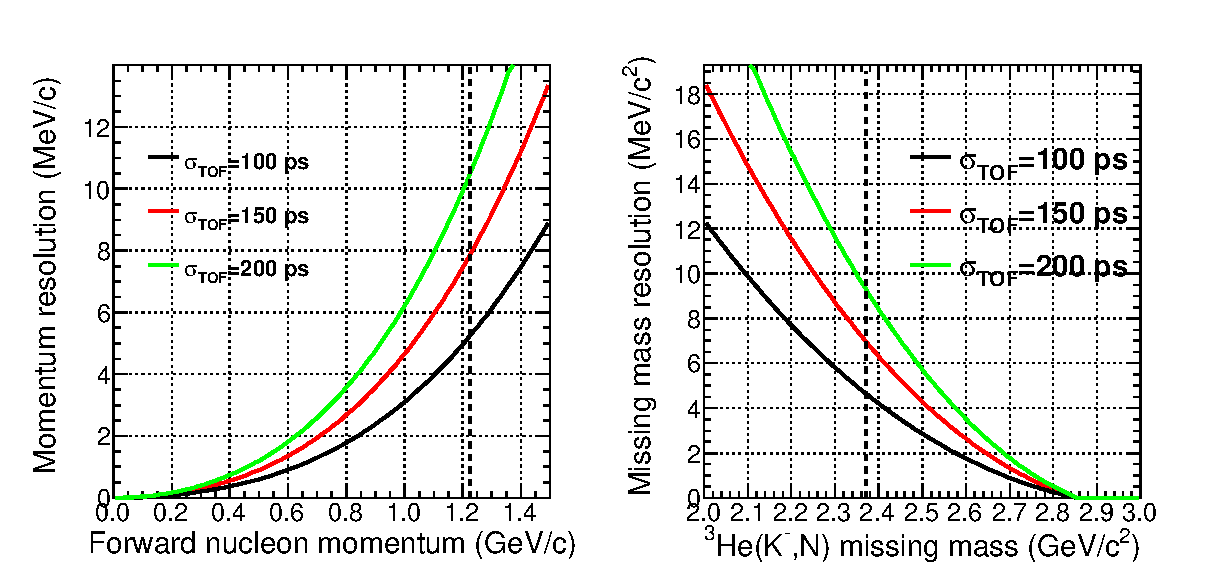
\includegraphics[width=\columnwidth]{fig/calcres.eps}
    \caption{Simple calculation of resolutions of the forward nucleon momentum and missing mass. }
    \label{fig-calcres}
   \end{center}
  \end{figure}  

\section{J-PARC}
Japan Proton Accelerator Research Complex (J-PARC), located at Tokai, Japan, is the only facility that provides a kaon beam today. The concept of J-PARC is to utilize secondary particles produced by primary proton beam of 1 MW class (design goal), which is the world highest intensity. J-PARC consists of three proton accelerators, an H$^-$ linac as an injector, 3 GeV Rapid Cycling Synchrotron (RCS), and 50 GeV Main Ring (MR). RCS acts as a booster for MR, and also delivers 3 GeV proton beam to the Material and Life science Facility, which aims at promoting material science and life science using pulsed neutron and muon beams. MR, now operating at 30 GeV, provides a fast extracted (FX) beam to produce neutrino beam to Kamioka and a slow extracted (SX) beam to the hadron experimental facility, where experiments of particle and nuclear physics are performed by using primary proton and secondary pion, kaon and anti-proton beams.

\subsection{SX beam and time structure}
In the SX operation, the beam in the MR is ``slowly" extracted by gradually shaving bunched beam while the remaining beam is kept circulating in the MR. The spill length was approximately two seconds with a six-second repetition cycle. 

The intensity of the SX beam in the present experiment was about 24 kW. It was about 10\% of the designed intensity. The difficulties to reduce the beam loss in the extraction process is one of the main reasons why the SX intensity is limited while the FX beam have already achieved more than 200 kW. 

Another problem is related to the time structure of the beam. %Hadron experiments with secondary beams require only 1 beam particle comes in the interested time range, often order 10 ns. That's why we use SX beam to suppress the instantaneous beam intensity while keeping integrated beam number. 
In an ideal case, the beam should be completely DC during the extraction period. However, we are suffering from a spike-like time structure on the extracted beam, which result from current ripples of the magnet power supplies in the MR.
To describe the spill time structure, we define the spill duty factor as
\begin{eqnarray}
Duty &= \left( \int_{0}^{T}I(t)dt\right)^2 / \int_{0}^{T}dt\int_{0}^{T}I(t)^2dt 
\end{eqnarray}
where $I(t)$ is the beam spill intensity, and $T$ is the spill length. The spill duty factor was $\sim$ 45\% in the experimental period with an application of 47.5 MHz transverse rf system. %\cite{transverse}
Microscopic time structures corresponding to the rf frequency was observed as is shown in the next chapter.   

A typical operation condition of the SX beam in May, 2013 is summarized in Table~\ref{table-sxbeam}.

\begin{table}[]
\caption{Typical operational condition of the SX beam as of May, 2013.}
\begin{center}
\begin{tabular}{ll}
\hline\hline
Primary beam momentum & 30 GeV/c \\
Primary beam power & 24 kW\\
~~Protons per spill & 3.0 $\times 10^{13}$ \\
~~Repetition cycle & 6 sec\\
%Flat Top & 2.93 sec\\
Spill Length & 2.1 sec\\
Spill duty factor & 45\% \\
Spill extraction efficiency & 99.5\% \\
Frequency of transverse RF & 47.5 MHz \\
\hline\hline
\end{tabular}
\end{center}
\label{table-sxbeam}
\end{table}%


\section{K1.8BR beam-line in the hadron experimental facility}
The primary proton beam is transported to a production target (T1) in the hadron experimental facility. In the present experiment, 6 mm (width) $\times$ 6 mm (height) $\times$ 66 mm (length) gold was used as the T1 target. The hadronic beams produced at the T1 target are extracted to several beam lines.

The present experiment is performed at the K1.8BR beam line located at the north side of the hadron experimental hall. The K1.8BR beam line is branched from the K1.8 beam line and has shorter beam line length of 31.3 m from the T1 target to the final focus point(FF), which is suitable to deliver low-momentum beam upto 1.2 GeV/$c$. The configuration of the K1.8BR beam line is shown in Fig.~\ref{k18br}, and its parameters are summarized in Table~\ref{k18brtable}.

The beam-line is composed of three sections: a front-end section (D1-D2), a mass separation section (IF-MS1), and a beam analyzer section (D3-FF). The front-end section is required for extraction of secondary particles from the T1 target. The extraction angle is chosen to be 6 degree, where the kaon production cross section is expected to be at a maximum according to the Sanford-Wang formula\cite{yamamoto1981}.

A good mass separation is realized with two vertical slits, an electrostatic separator (ES1), and a pair of correction magnets. The secondary beam is focused vertically at the entrance of mass separation section, where an IF-V slit is placed to reduce so-called cloud pion and to redefine the beam size. Then the 6 m-long ES1 vertically separates the particle trajectory by their mass with an applied field of 50 kV/cm\cite{Ieiri20084205}. Finally, a vertical slit (MS1) pass through the selected mass beam with a help of two vertical steering magnets, CM1 and CM2. We also have two horizontal slits, an IF-H at the internal focus point and a MOM just downstream of the MS1, where the optics is designed to be dispersive. 

After the D3 magnet, an SQDQD system is employed to focus the beam on the experimental target at FF of the K1.8BR beam line. The most downstream magnet D5 is required to change the beam direction to keep a flight-length of scattered neutron as long as 15 m. The D5 magnet is also used as a beam momentum analyzer. 

The first-order beam envelope calculated by the TRANSPORT code\cite{Anonymous:M8WJFLy5} is shown in Fig. \ref{fig-optics}.
\begin{figure}[]
\begin{center}
\includegraphics[width=25pc]{fig/k18br.eps}
\caption{\label{k18br} Schematic drawing of K1.8BR beam line in the J-PARC hadron experimental facility.}
\end{center}
\end{figure}

\begin{figure}[]
\begin{center}
\includegraphics[width=0.9\columnwidth]{illustrator/optics.eps}
\caption{\label{fig-optics} First-order beam envelope.}
\end{center}
\end{figure}

\begin{table}[]
\caption{Parameters of K1.8BR beam line as of May, 2013.}
\begin{center}
\begin{tabular}{ll}
\hline\hline
Production target & Au (50\% loss)\\
Extraction Angle & 6$^\circ$ \\ 
Momentum range & 1.2 GeV/c max.\\
Acceptance & 2.0 msr $\cdot$ \%\\
Momentum bite & $\pm$ 3 \%\\
Beam Length (T1-FF) & 31.3 m\\
\hline\hline
\end{tabular}
\end{center}
\label{k18brtable}
\end{table}%

\subsection{Kaon beam tuning}
Kaon beam tune was performed to maximize the number of kaons on the experimental target while keeping a pion contamination to the acceptable level.

After the establishment of online particle identification triggers, we optimized the combination of ES1, CM1 and CM2 setting to maximize the kaon yield. Then the center of the vertical beam position was measured by changing two vertical slit positions. The horizontal position of beam was optimized by D3,D4 and D5 with a narrowed setting for the momentum slit. Currents of quadruple magnets were also scanned to increase the kaon yield and for better focus at FF. Finally, opening widths of two vertical slits and two horizontal slits were optimized in terms of a $K/\pi$ ratio and a total beam intensity.

A typical kaon intensity during the experimental period was 1.5 $\times 10^5$ per spill with the $K^-/\pi^-$ ratio of $\sim$0.45. The optimized magnet settings and slit settings are summarized in Table \ref{tab-magnet} and Table \ref{tab-slit}, respectively.

%The obtained setting of each magnet is tabulated in Table \ref{table-mag} with designed values by optical calculation code TRANSPORT, while the optimized slit setting and a typical beam typical parameters are summarized in Table \ref{table-slit} and Table \ref{table-beam}, respectively.  More detailed property of the beam will appear in Appendix.



\begin{table}[]
\caption[Parameters of the beam-line magnets.]{Parameters of the beam-line magnets. D5 field is a typical monitored value. Other field values are interpolations of measured points.}
\begin{center}
\begin{tabular}{llccccc}
\hline\hline													
Element	&	J-PARC	&	Gap or	&	Effective	&	Bend	&	Current	&	Field at pole	\\
	&	designation	&	 bore/2 (cm)	&	length (cm)	&	(deg)	&	(A)	&	(kG)	\\
\hline													
D1	&	5C216SMIC	&	8	&	90.05	&	10	&	-365$\sim$-374	&	-6.5808$\sim$-6.7444	\\
Q1	&	NQ312MIC	&	8	&	67.84	&		&	-357	&	-3.075	\\
Q2	&	Q416MIC	&	10	&	87.04	&		&	-668	&	3.872	\\
D2	&	8D218SMIC	&	15	&	99.65	&	15	&	-698	&	-8.7673	\\
\hline
IF-H	&	\multicolumn{4}{l}{Movable horizontal slit for acceptance control}		&		&		\\
IF-V	&	\multicolumn{4}{l}{Movable vertical slit, (y$|\phi$)=0}					&		&		\\
\hline
Q3	&	Q410	&	10	&	54.72	&		&	-679	&	-4.108	\\
O1	&	O503	&	12.5	&	15	&		&	-15	&	-0.29	\\
Q4	&	Q410	&	10	&	54.72	&		&	-776	&	4.692	\\
S1	&	SX504	&	12.5	&	27.6	&		&	-42	&	-0.29	\\
CM1	&	4D604V	&	10	&	20	&	(0.856)	&	419	&	1.943	\\
ES1	&	Separator	&	10	&	600	&		&	\multicolumn{2}{c}{E=-500 kV/10 cm}	\\
CM2	&	4D604V	&	10	&	20	&	(0.856)	&	419	&	1.940	\\
S2	&	SX504	&	12.5	&	27.6	&		&	-136	&	1.02	\\
Q5	&	NQ510	&	12.5	&	56	&		&	-498	&	4.218	\\
Q6	&	NQ610	&	15	&	57.2	&		&	-535	&	-4.316	\\
\hline
MOM	&	\multicolumn{5}{l}{Movable horizontal slit for momentum acceptance control}		&		\\
MS1	&	\multicolumn{4}{l}{Movable vertical slit for $K$-$\pi$ separation }					&		&		\\
	&	\multicolumn{4}{l}{($y|\phi$)=0, ($y|y$)=0.844, ($y|\theta\phi$)=($y|\phi\delta$)=0} 		&		&		\\
\hline
D3	&	6D330S	&	15	&	165.1	&	20	&	210	&	-7.064	\\
S3	&	SX404	&	10	&	20	&		&	-34	&	-1.062	\\
Q7	&	Q306	&	7.5	&	30.34	&		&	-464	&	4.026	\\
D4	&	8D440S	&	20	&	198.9	&	60	&	-1936	&	-17.8907	\\
Q8	&	NQ408	&	10	&	46.5	&		&	-110	&	0.671	\\
D5	&	8D240S	&	20	&	195.9	&	55	&	-1663	&	-16.413	\\
\hline\hline													
\end{tabular}
\end{center}
\label{tab-magnet}
\end{table}%


\begin{table}[]
\caption[Optimized slit settings.]{Optimized slit settings. All unit in mm.}
\begin{center}
\begin{tabular}{lcc}
\hline\hline					
IF-H	&	110	&	-110	\\
IF-V	&	2.5	&	-1.1	\\
Mass	&	1.75	&	-2.45	\\
Mom	&	L 160.0	&	R -110.0	\\
\hline\hline
\end{tabular}
\end{center}
\label{tab-slit}
\end{table}%
\section{Beamline}

\subsection{BHD and T0}
The beam particles are kaon is confirmed by the TOF method using beamline hodoscope detector (BHD) and time-zero counter (T0) in the offline analysis.
The T0 is located immediately downstream of the AC.
The BHD is located between the D5 and D4 magnets, approximately 7.7m upstream of T0, i.e. the flight length is 7.7m.

The T0 is a 5-segment plastic scintillation counter array 160mm (high) $\times$ 32mm (width) $\times$ 10mm (thick), with an effective area of 160mm $\times$ 160mm.
The T0 is installed rotated 45 degrees with respect to the beam direction as the beam is horizontally spread at the T0.
A counter uses the Saint-Gobain BC420 scintillator and attached readout which is 3/4 inch Hamamatsu H6612B photomultipliers to both sides of the scintillator.

The BHD is a 20-segment plastic scintillation counter array 160mm (high) $\times$ 20mm (width) $\times$ 5mm (thick), with an effective area of 200mm (horizontal) $\times$ 160mm (vertical).
A counter uses the same photomultipliers as the T0 counter.
The BHD is installed at the most upstream of the beamline and the number of beams per spill is a few M ($\times 10^6$)events,
so the photomultipliers are attached high voltage booster to the last three dynodes to avoid gain drop due to high current by high rate beam.

\subsection{Beam line chamger}
\begin{figure}[htbp]
  \centering
  \begin{tabular}{ccc}
    \begin{minipage}{0.33\hsize}
      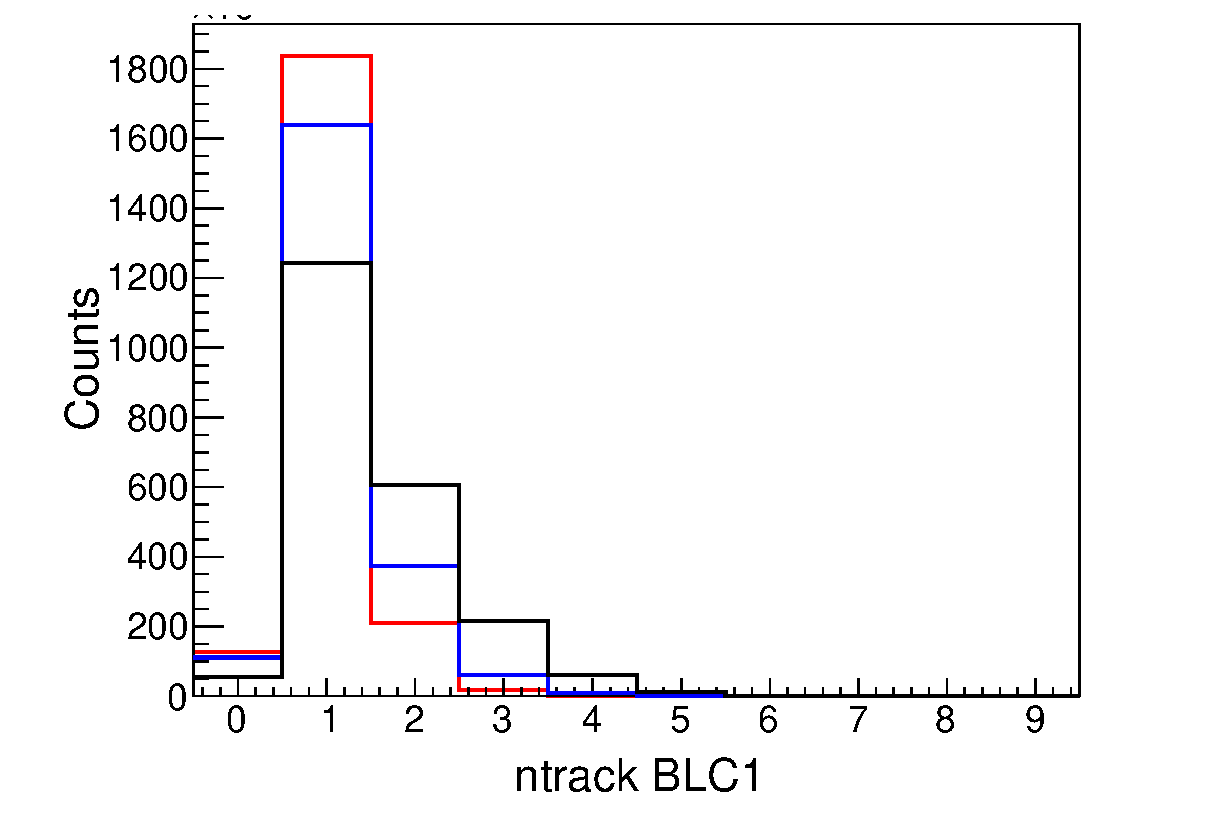
\includegraphics[width=4cm]{../pic/Run78/BL/nBLC1.eps}
    \end{minipage}
    \begin{minipage}{0.33\hsize}
      \includegraphics[width=4cm]{../pic/Run78/BL/BLC1_time.eps}
    \end{minipage}
    \begin{minipage}{0.33\hsize}
      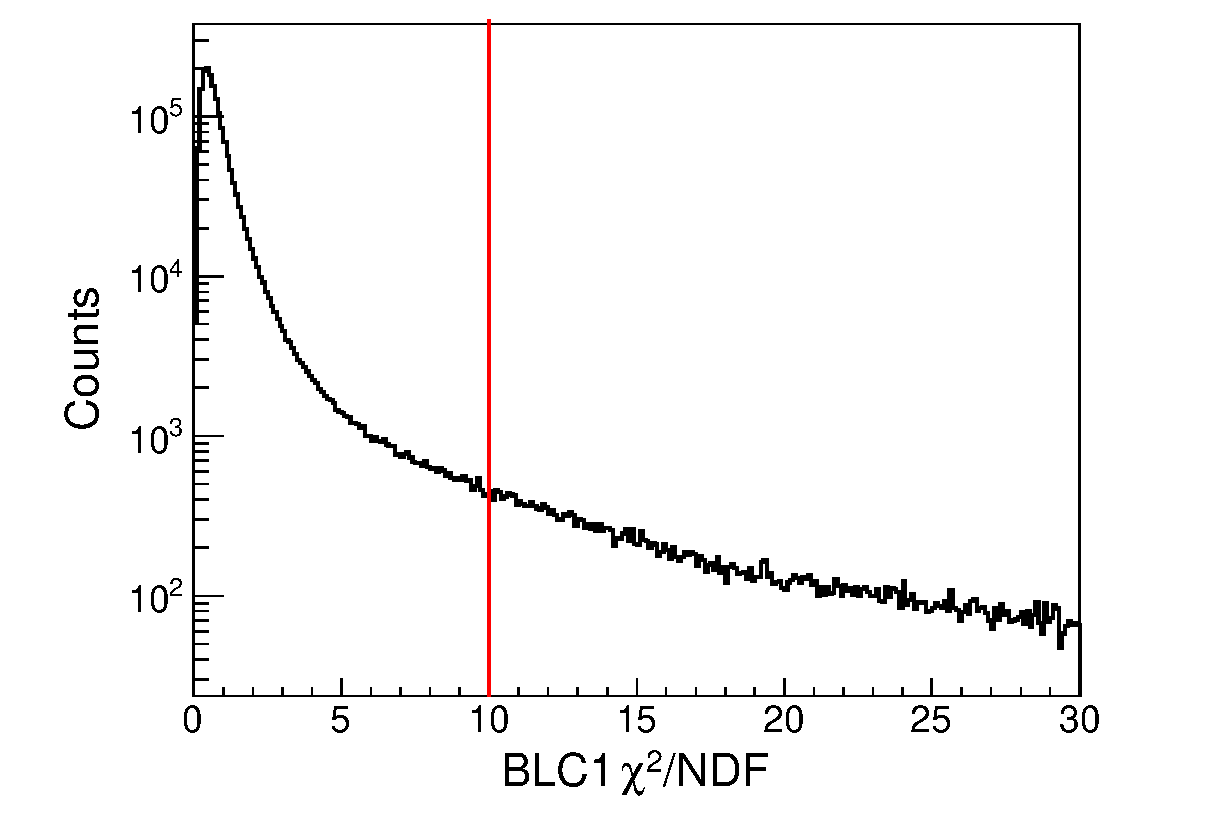
\includegraphics[width=4cm]{../pic/Run78/BL/BLC1_chi2.eps}
    \end{minipage}
  \end{tabular}
  
  \begin{tabular}{ccc}
    \begin{minipage}{0.33\hsize}
      \includegraphics[width=4cm]{../pic/Run78/BL/nBLC2.eps}
    \end{minipage}
    \begin{minipage}{0.33\hsize}
      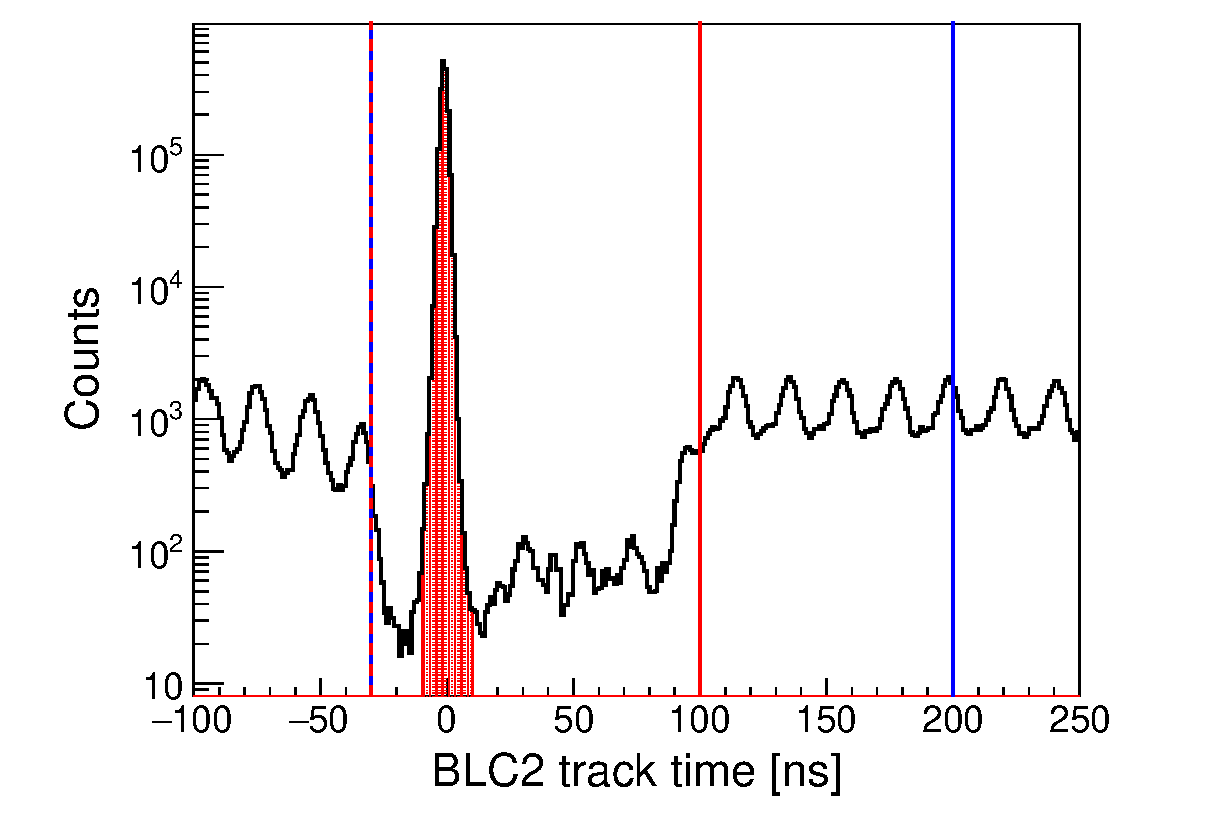
\includegraphics[width=4cm]{../pic/Run78/BL/BLC2_time.eps}
    \end{minipage}
    \begin{minipage}{0.33\hsize}
      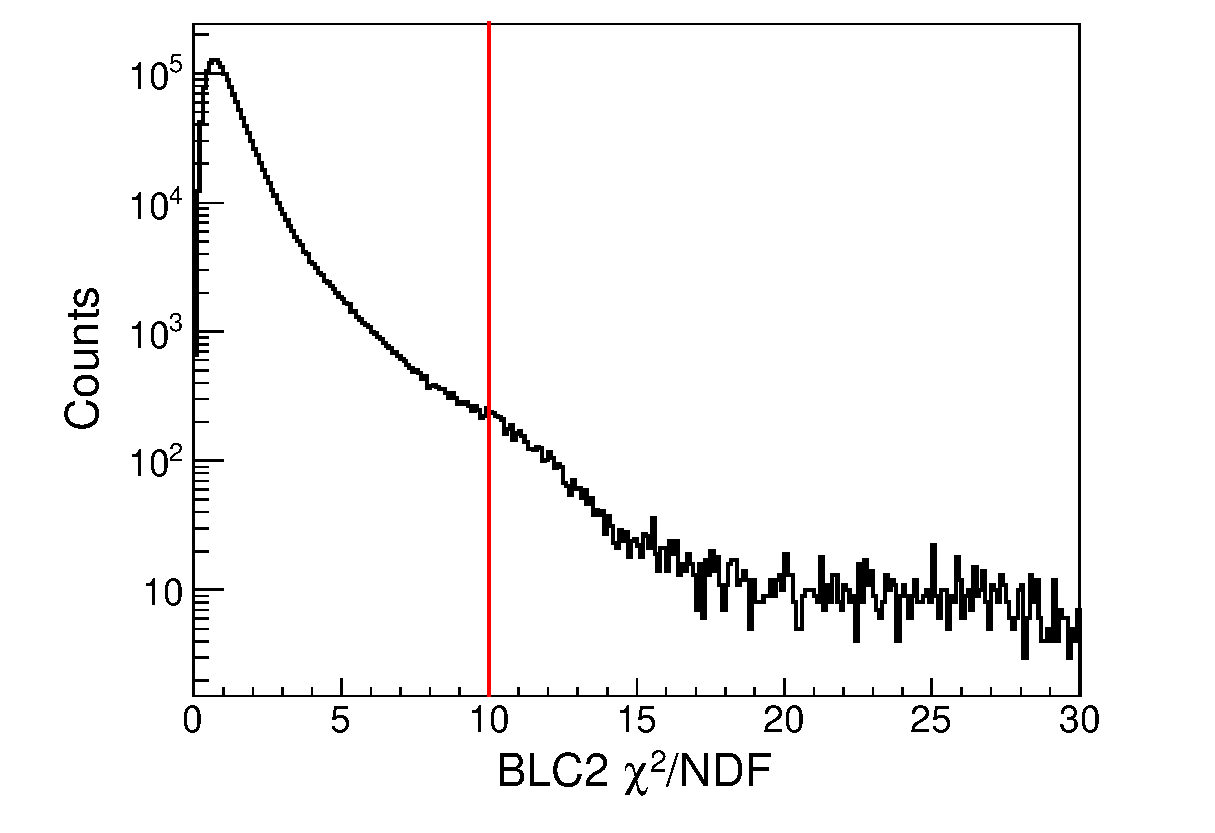
\includegraphics[width=4cm]{../pic/Run78/BL/BLC2_chi2.eps}
    \end{minipage}
  \end{tabular}
  
  \begin{tabular}{ccc}
    \begin{minipage}{0.33\hsize}
      \includegraphics[width=4cm]{../pic/Run78/BL/nBPC.eps}
    \end{minipage}
    \begin{minipage}{0.33\hsize}
      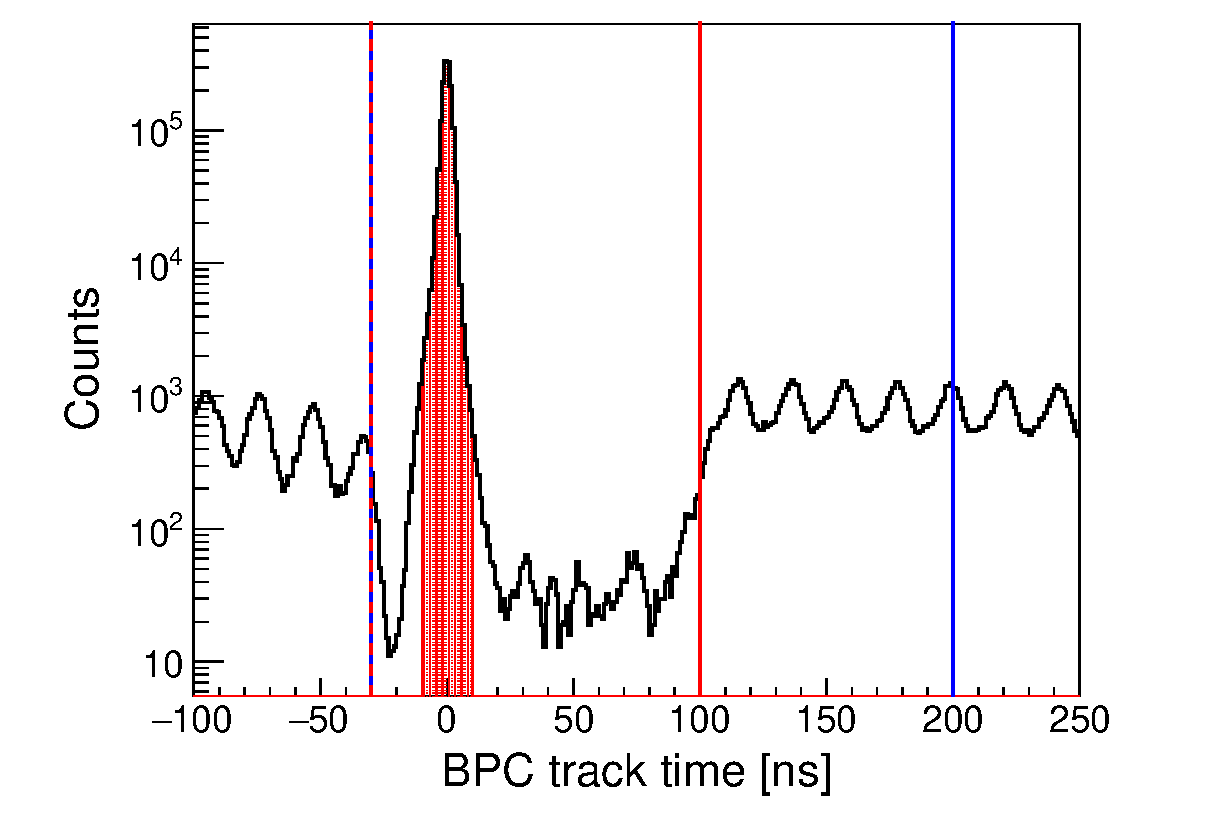
\includegraphics[width=4cm]{../pic/Run78/BL/BPC_time.eps}
    \end{minipage}
    \begin{minipage}{0.33\hsize}
      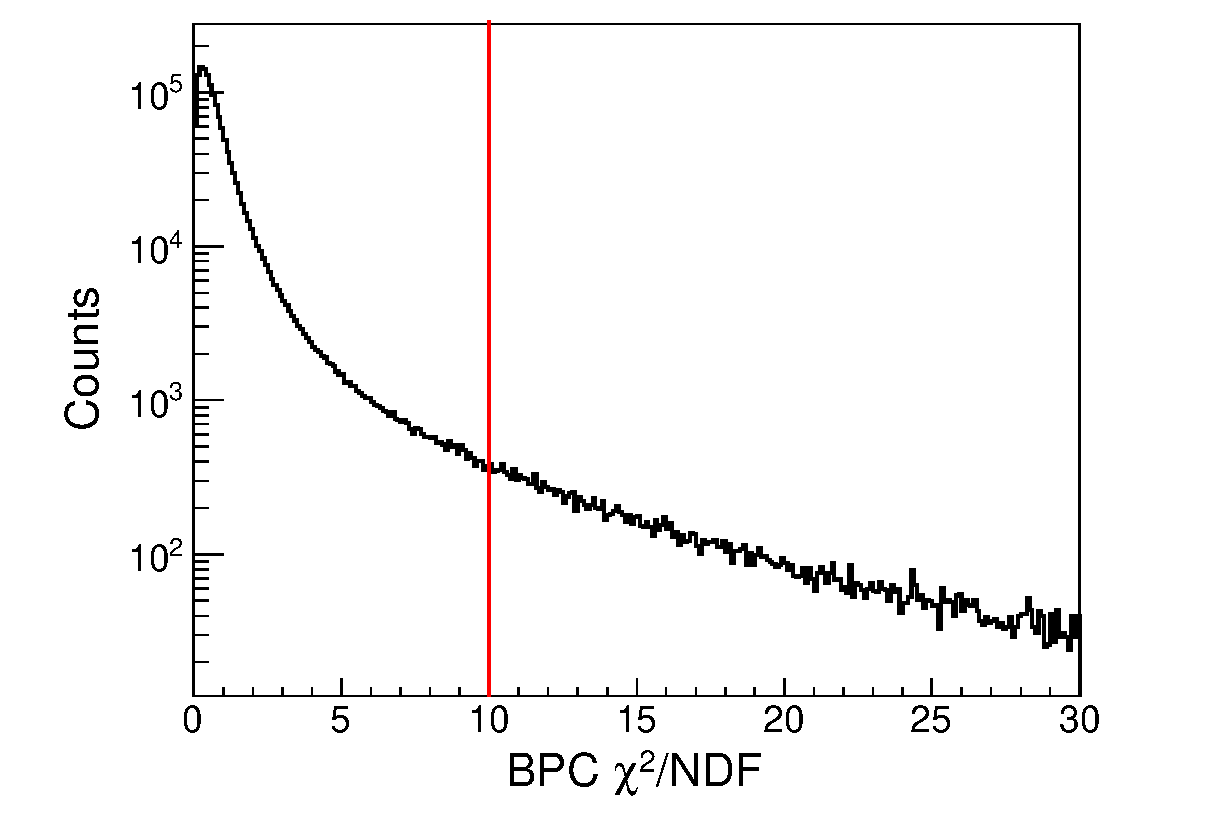
\includegraphics[width=4cm]{../pic/Run78/BL/BPC_chi2.eps}
    \end{minipage}
  \end{tabular}
  \caption{
    The left, the middle and the right figures show the number of tracks, track time and $\chi/NDF$, respectively.
    Color plots in the left figure indicate some time window.
    % Black, blue, red indicate all, $-30\sim200$[ns], $-30\sim100$[ns], respectively.
    The above, the middle and the down figures represent BLC1, BLC2 and BPC, respectively.
    The BPC was described after.
  }
  \label{fig:BLC_etc}
\end{figure}
BLC1 and BLC2 were installed upstream and downstream of the D5 magnet, respectively to measure beam momentum using the transfer matrix of the D5 magnet.
These are planer the type drift chamber whose drift length was calculated using the X-T map, which was the integration of drift time.
The track time of BLC was estimated from timing signals of pair plane due to constant drift length.
SX beam has RF-structure seems like the center figures of Fig\ref{fig:BLC_etc}, so we select synchronization about beam which indicates the red hatched region.
The left figures represent the number of tracks, in which black, blue, and red indicate time window of all, $-30\sim100$[ns], and $-30\sim200$[ns], respectively.
We select 1track events in red time window selection to keep statistics.
The right figures show $\chi^2/NDF$ distribution after 1track selection.
We accepted $\chi^2/NDF<10$ events as good track.



%\subsection{Liquid $^3$He target system} 
\subsubsection{Configuration and operational procedure} 
A schematic drawing of the liquid $^3$He cryostat is shown in Fig. \ref{lhe3:cryo} for the case of the J-PARC E15 setup. 
The details of the $^3$He target system can be found in a separate paper \cite{Iio12}. 
The major difference between the E15 and E17 settings is the configuration around the target cell. 
To maximize the acceptance for the kaonic helium X-rays in E17,  eight silicon drift detectors (SDDs) will be installed around the target cell as shown
 in the inset of Fig. \ref{lhe3:cryo}. 
In contrast, a time projection chamber will be installed between the target vacuum chamber and the CDS in the E15 setup.  
Thus, the diameter of the vacuum chamber is minimized as much as possible.
The major cryogenic component is divided into three sections; a $^4$He separator,  a $^4$He evaporator and  a heat exchanger between $^3$He and $^4$He.
The target cell is connected to the bottom of the heat exchanger with two 1 meter long pipes.
To reduce the radiation from room temperature components, all low-temperature parts are covered with a radiation shield  anchored to the liquid nitrogen tank (LN$_2$ tank). 

%%operation
The operational concept of the cryostat of E15 and E17 is essentially the same. 
Typical start-up procedure begins with liquid nitrogen cooling. 
When the $^4$He separator and the LN$_2$ tank are filled, the evaporator, the heat exchanger and the target cell are cooled by thermal conduction and radiation.
After the pre-cooling, the liquid nitrogen in the separator is purged, and the liquid helium is transferred from a 1000 $\ell$ Dewar (not shown in the figure) to the separator by a transfer tube. 
The liquid flow is controlled by the pressure inside the separator evacuated by a dry pump. Liquid $^4$He inside the separator is fed to the $^4$He evaporator though a needle valve.
The vapor pressure in the evaporator is reduced by a rotary pump with pumping speed of 120 m$^3$/h, resulting in a heat-removal capability of 2.5 W at 2 K. 
The temperature inside the evaporator is controlled within a range of  1.3 to 2.0 K. This range is mainly determined by the flow rate from the separator to the evaporator. The lowest temperature is achieved with no flow from the separator because the liquid temperature in the separator is fairly high (4.2 K). For liquefaction of $^3$He, the heat exchanger between liquid $^4$He and gaseous $^3$He is positioned below the evaporator. The top part of the heat exchanger, where the liquid $^4$He in the evaporator is in direct contact, has a specially-designed fin structure with both a width and pitch of 0.5 mm. 

A gas-tight handling system (leak rate less than 10$^{-10}$ Pa$\cdot$m$^3$/sec)
 has been constructed to store, transfer and recover the scarce $^3$He gas.
The total amount of 400 $\ell$ of gaseous $^3$He is stored at pressures of less than an atmosphere at room temperature in two 200 $\ell$ tanks. During the cooling stage, those gas tanks are connected to the heat exchanger through the gas handling system.  
 By an effective heat contact inside the heat exchanger, gaseous $^3$He is liquefied, and the liquid $^3$He is flowed to the target cell (6.8~cm in diameter and 13.7~cm in length) through the lower pipe.
 At the last stage of the cooling, most of the $^3$He gas is liquefied inside the target cell and the heat exchanger. 

%%% siphon method %%%
In the L-shaped cryostat, the heat load on the target cell must be transferred effectively to the heat exchanger where the cooling power exists. Otherwise boiling in the target cell occurs.
To accomplish this, we applied the {\it siphon method} as described in Ref. \cite{Iio12}, which uses convection of the liquid $^3$He.
The liquid $^3$He warmed by the heat load inside the target cell returns to the heat exchanger through an upper pipe. In the heat exchanger, $^3$He is cooled again and fed to the target cell through the lower pipe. This makes possible the heat transfer between the target cell and the heat exchanger.  

%%% one shot %%%
For long-term operation, it is essential to reduce the total amount of $^4$He consumed. This is because exchanging the $^4$He Dewar causes significant experimental dead time. 
To minimize the $^4$He consumption, we adopted {\it one-shot} operation. 
This operation consists of two modes;
(I) the evaporator is filled up with liquid $^4$He supplied from the separator. (II) The $^4$He supply is stopped until the evaporator becomes empty. 
The operational procedure consists of a repetition of these two methods, and 
this reduces the total liquid $^4$He consumption due to the minimization of the transfer loss to the cryostat. 
The operational performance of the target system is described in the following.

\begin{figure}[t]
\includegraphics[width=\columnwidth]{lhe3-cryo.eps}
\caption{ \label{lhe3:cryo}
Schematic drawing of the liquid $^3$He cryostat.
}
\end{figure}
%%%%%%%%%%%%%%%%%%%%%%%%%%%%%%%%%%%%%%%%%%%%%%%%%%%%%%%%%%%%%%%%%%%%%%%%%%%%%%

%\subsubsection{$^3$He target cell} 
% Since kaonic helium $L_{\alpha}$ X-rays have an energy of 6 keV, they are easy to be absorbed in the target cell before detection by X-ray detectors. 
%The choice of the material of the target cell is extremely important.
%We have developed the target cell made of pure beryllium. 
%%The detailed configuration is found in Ref. \cite{Iio12}. 
%The target cell has a cylindrical shape of 68 mm diameter and 138 cm long. 
%The side wall is made of pure beryllium of 0.3 mm thick. 
%The volume of the target cell is 0.48 $\ell$ in which the volume of 269 $\ell$ gaseous $^3$He at room temperature is necessary to fill up with liquid at 1.3 K.
%The purity of the beryllium cylinder is more than 99.4 \%, and the transmittance of 5.9 keV X-rays are confirmed to be $85.3\pm 1.0$ \% by manganese  $K_{\alpha}$ X-rays from radioactive $^{55}$Fe source. 
%This is comparable with that of pure beryllium of 87.2 \%.

%\subsubsection{Vacuum chamber} 
%A vacuum chamber was specially designed to reduce multiple scattering of secondary charged particles.
%As a result of the development in KEK \cite{Sato09}, the material of the vacuum chamber was carefully selected to Carbon Fiber Reinforced Plastic (CFRP) in the region covering the acceptance of the CDS. 
%The detail of the specification of adopted CFRP is found in Ref. \cite{Iio12}.
%Total thickness of the CFRP in the E15 setup is 1 mm with the diameter of 150 mm and the length of 523 mm. 
% An aluminum beam window with the thickness of 0.6 mm is glued to the CFRP with STYCAST 1266.
%A safety factor of this vacuum chamber is estimated to be 3.8 against the external pressure of 1 atm. 

\subsubsection{Operation and performance} 
Along with the operational procedure previously described, cooling tests were performed. 
After the $^4$He transfer, it took about 2 - 3 hours to liquefy  the $^3$He gas in the heat exchanger, achieving thermal equilibrium within 6 hours and a temperature of 1.30 $\pm$ 0.01 K in the target cell without flow from the separator (mode (II) in the {\it one-shot} operation).
The liquid $^3$He density at this temperature is 0.0812~g/cm$^3$ corresponding to the thickness of 1.11~g/cm$^2$.
The density fluctuation due to the temperature instability is less than 0.1 \%.
The temperature differences among the evaporator, the heat exchanger and the target cell are less than 0.01 K. This means the heat transfer by {\it siphon method} is working well.
Furthermore, the pressure inside the heat exchanger was identical to the vapor pressure of liquid $^3$He at the corresponding temperature. Taking into consideration the remaining pressure inside the tanks, a total amount of 380 $\ell$ was condensed, giving evidence that sufficient $^3$He gas is liquefied to fill the target.

From the reduction rate of the liquid $^4$He in the evaporator, 
the heat load of the low-temperature region was estimated to be 0.21 W with the E15 setting.
In the E17 setting, the heat load was expected to increase due to the radiation from the SDDs to the target. 
It was measured to be 0.39 W with the actual E17 setting, and both of them are acceptably small for long-term operation.
The  operational result of the cryostat with the E15 setting is tabulated below.

\begin{table}[h] 
\begin{center}
\caption{\label{operation}Operational result.}
\begin{tabular}{lrc}\hline\hline
vacuum level                      & [mbar]                 &$ < 10^{-6}$ \\ 
leak rate of the $^3$He system    & [Pa$\cdot$m$^3$/sec] &$< 10^{-10}$ \\ 
temperature in the target cell    &[K]       & 1.3        \\
vapor pressure in the target            &[mbar]    & 33         \\
heat load to low-temperature part   &[W]       & 0.21       \\ 
liquid $^4$He consumption          &($\ell$/day)      & 50         \\ 
 \hline \hline  
\end{tabular}
\end{center}
\end{table}
Finally, we note that this cryostat can be utilized as a liquid $^4$He target system by liquefying gaseous $^4$He instead of $^3$He. The operational procedure and the performance of the liquid $^4$He target are the same as those of $^3$He.
The density of the liquid $^4$He is 0.145~g/cm$^3$ at 1.3~K with a stability of better than 0.1 \%, and the thickness is 1.99 g/cm$^2$. 



%%%  References
% M. Iio et al., submitted to Nucl. Instr. and Meth. A
% M. Sato et al., Nucl. Instr. and Meth. A 606 (2009) 233 

%===============================%
\section{Cylindrical detector system}
%===============================%
A schematic view of the cylindrical detector system (CDS) with the target system is shown in Fig.~\ref{fig:CDS}.
Charged particles generated by the reaction at the target are reconstructed by a cylindrical drift chamber (CDC), which operates in a magnetic field of 0.7~T provided by a solenoid magnet. A cylindrical detector hodoscope (CDH) is used for particle identification and as a charged particle trigger. An inner hodoscope (IH) is installed to enlarge the acceptance for the tracks out of CDH acceptance. The DEF and BPC, which are already described in Sec. 2.6, are located just upstream of the target chamber. A backward proton detector (BPD) is installed to detect backward scattered particles for another experiment

  \begin{figure}[]
   \begin{center}
    \includegraphics[width=\columnwidth]{./fig/cds_v4.eps}
    \caption{Schematic drawing of the CDS with the target system.}
    \label{fig:CDS}
   \end{center}
  \end{figure}  

\subsection{Solenoid magnet}
The spectrometer magnet of the CDS is of a solenoidal type, whose bore diameter is 1.18~m and whose length is 1.17~m with an overall weight of 23 tons. 
The design of the solenoid magnet is shown in Fig.~\ref{fig:solenoid}. It is located on the final focus point of the K1.8BR beam line. The magnet provides a uniform field strength inside the tracking volume ($|z| <$ 420~mm). In the present experiment, it is operated at 0.7 T.

  \begin{figure}[htbp]
   \begin{center}
    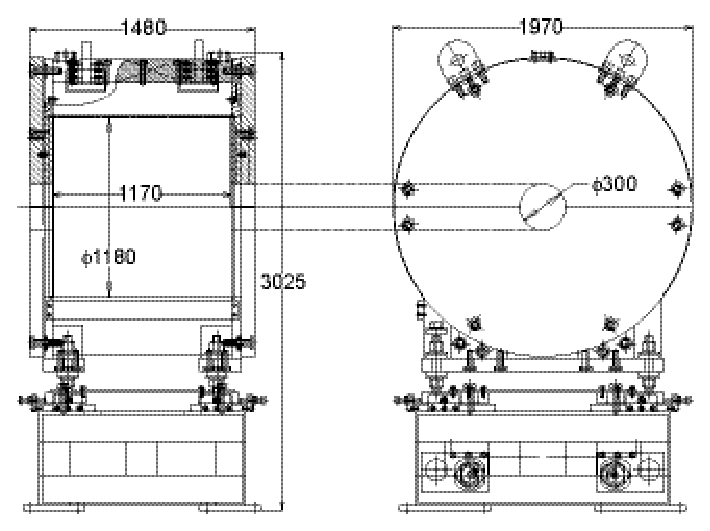
\includegraphics[width=0.8\columnwidth]{ptep/fig/solenoid.eps}
    \caption[Design of the solenoid magnet]{Design of the solenoid magnet (all dimensions in mm).}
    \label{fig:solenoid}
   \end{center}
  \end{figure}  

\subsection{Cylindrical drift chamber}
The CDC is a cylindrical wire drift chamber that contains 15 layers of anode wires. The structure of the CDC is shown in Fig.~\ref{fig:CDC_structure}.
The outer radius is 530~mm and the inner radius is 150~mm, with a total length of 950~mm. The wire length of axial layers is 833.8~mm, thus the angular coverage is 49$^\circ$ $< \theta <$ 131$^\circ$ in the polar angle region corresponding to a solid angle coverage of 66\% of 4$\pi$.
The CDC consists of two aluminum end-plates of 20~mm thickness, a 1~mm thick CFRP cylinder as the inner wall of the CDC, and six aluminum
posts that are placed outside the tracking volume. The CDC uses gold-plated tungsten of 30~$\mu$m$~\phi$ for the sense wires, and gold-plated aluminum of 100~$\mu$m$~\phi$ for the field and guard wires. These wires are supported by feedthroughs with a bushing inserted at the end. Bushes with an 80 and 200 $\mu$m$~\phi$ hole are used for the sense and field/guard wires, respectively.

The CDC has 15 layers of small hexagonal cells with a typical drift length of 9~mm, which are grouped into 7 super-layers as shown in
Fig.~\ref{fig:CDC_cell}. Table~\ref{tab:CDC} gives the detailed parameters of the wire configuration. The layers are in the radial region from 190.5~mm (layer \#1) to 484.5~mm (layer \#15). The 8 stereo layers tilted by about 3.5$^\circ$ are used to obtain longitudinal position information. The number of readout channels is 1816 and the total number of wires in the CDC is 8064.

  \begin{figure}[]
   \begin{center}
    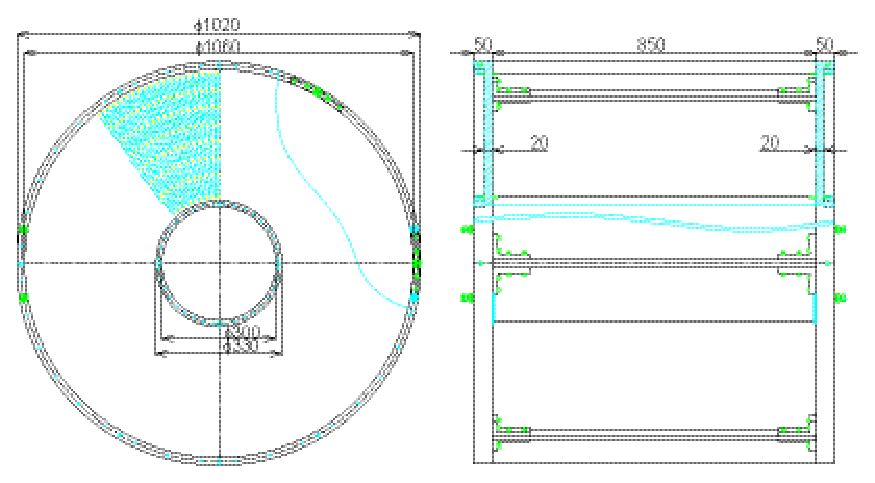
\includegraphics[width=0.8\columnwidth]{ptep/fig/CDC_structure.eps}
    \caption[Design of the CDC.]{Design of the CDC (all dimensions in mm).
    The CDC consists of two aluminum end-plates, a 1~mm thick CFRP
    cylinder as an inner wall, and six aluminum posts that are placed
    outside the tracking volume.}
    \label{fig:CDC_structure}
   \end{center}
  \end{figure}  

  \begin{figure}[]
   \begin{center}
    \includegraphics[width=0.5\columnwidth]{ptep/fig/CDC_cell.eps}
    \caption{Cell structure of the CDC.}
    \label{fig:CDC_cell}
   \end{center}
  \end{figure}  

 \begin{table}[]
  \begin{center}
   \caption{Wire configuration of the CDC.}
   \label{tab:CDC}
   \begin{tabular}{cccccccc}
\hline	\hline														
Super-	&	\multirow{2}{*}{layer}	&	Wire	&	Radius	&	\multicolumn{2}{c}{Cell width}			&	\small{Stereo angle}	&	Signal	\\
layer	&		&	direction	&	(mm)	&	(degree)	&	(mm)	&	(degree)	&	channels	\\
\hline															
\multirow{3}{*}{A1}	&	1	&	$X$	&	190.5	&	\multirow{3}{*}{5.00}	&	16.7	&	0	&	72	\\
	&	2	&	$X'$	&	204	&		&	17.8	&	0	&	72	\\
	&	3	&	$X$	&	217.5	&		&	19	&	0	&	72	\\
\hline															
\multirow{2}{*}{U1}	&	4	&	$U$	&	248.5	&	\multirow{2}{*}{4.00}	&	17.3	&	-3.55	&	90	\\
	&	5	&	$U'$	&	262	&		&	18.3	&	-3.74	&	90	\\
\hline															
\multirow{2}{*}{V1}	&	6	&	$V$	&	293	&	\multirow{2}{*}{3.60}	&	18.4	&	3.77	&	100	\\
	&	7	&	$V'$	&	306.5	&		&	19.3	&	3.94	&	100	\\
\hline															
\multirow{2}{*}{A2}	&	8	&	$X$	&	337.5	&	\multirow{2}{*}{3.00}	&	17.7	&	0	&	120	\\
	&	9	&	$X'$	&	351	&		&	18.4	&	0	&	120	\\
\hline															
\multirow{2}{*}{U2}	&	10	&	$U$	&	382	&	\multirow{2}{*}{2.40}	&	16	&	-3.28	&	150	\\
	&	11	&	$U'$	&	395.5	&		&	16.6	&	-3.39	&	150	\\
\hline															
\multirow{2}{*}{V2}	&	12	&	$V$	&	426.5	&	\multirow{2}{*}{2.25}	&	16.7	&	3.43	&	160	\\
	&	13	&	$V'$	&	440	&		&	17.3	&	3.54	&	160	\\
\hline															
\multirow{2}{*}{A3}	&	14	&	$X$	&	471	&	\multirow{2}{*}{2.00}	&	16.4	&	0	&	180	\\
	&	15	&	$X'$	&	484.5	&		&	16.9	&	0	&	180	\\
\hline\hline
   \end{tabular}
  \end{center}
 \end{table}

The drift gas is 1 atm of mixed argon (50\%)-ethane (50\%). A high voltage is applied to the field and guard wires, and the sense wires are kept at ground potential. For the first super-layer (A1) and the second one (U1), a high voltage of -2.8 kV is applied to the potential wires, and -2.7 kV to the potential wires of the other super-layers. In addition, -1.5 kV, -1.8 kV, and -0.6 kV are applied to the innermost, the outermost, and the other guard wires, respectively.
The readout electronics of the CDC consists of a preamp card with ASDs (SONY-CXA3653Q, $\tau$ = 16~ns), an LVDS-ECL converter, and a TDC --
the same as those for the beam line chambers. 

\subsection{Cylindrical detector hodoscope}
The CDH is a segmented plastic scintillation counter used for the charged
particle trigger and particle identification.
The CDH is located at a radius of 544~mm from the beam axis covering
a polar angle range from 54 to 126 degrees corresponding to a solid
angle coverage of 59\% of 4$\pi$.

The CDH consists of 36 modules, individually mounted on the inner wall
of the solenoid magnet.
The scintillators are made of Eljen EJ-200, with dimensions of 790~mm
in length, 99~mm in width, and 30~mm in thickness.
The scintillation light is transferred through light guides to a pair of
Hamamatsu R7761 fine-mesh 19-dynode photomultipliers 1.5 inches in
diameter.

The CDH is operated in the 0.7~T magnetic field with a typical PMT gain
of $\sim10^6$. 
The measured average time resolution of the CDH without a magnetic field
is 71 $\pm$ 3 ~ps ($\sigma$), obtained with cosmic ray data. 
The error represents the variation among the segments.

\subsection{Inner Hodoscope}
An inner hodoscope (IH) is a segmented plastic scintillation counter mounted on the inner wall of the CFRP cylinder of the CDC at a radius of 140~mm from the beam axis. The IH covers a polar angle range from 27 to 153 degrees corresponding to a solid angle coverage of 89\% of 4$\pi$.

The IH consists of 24 ELJEN EJ-200 scintillators with dimensions of 600~mm in length, 37~mm in width, and 3~mm in thickness. Each segment is overlapped by 1 mm. % as shown in Fig. \ref{fig-IH}. 
Due to the strong magnetic field and a limited space, multi-pixel photon counters (MPPCs) with a 3 mm $\times$ 3 mm sensitive area were used (Hamamatsu S10362-33-100C). The scintillation light is collected by 4 wavelength-shifting fibers embedded in the scintillator and connected to an MPPC with a specially designed connector. The MPPC signal is read out by using a preamplifier (HOSHIN). 

\if0
  \begin{figure}[]
   \begin{center}
    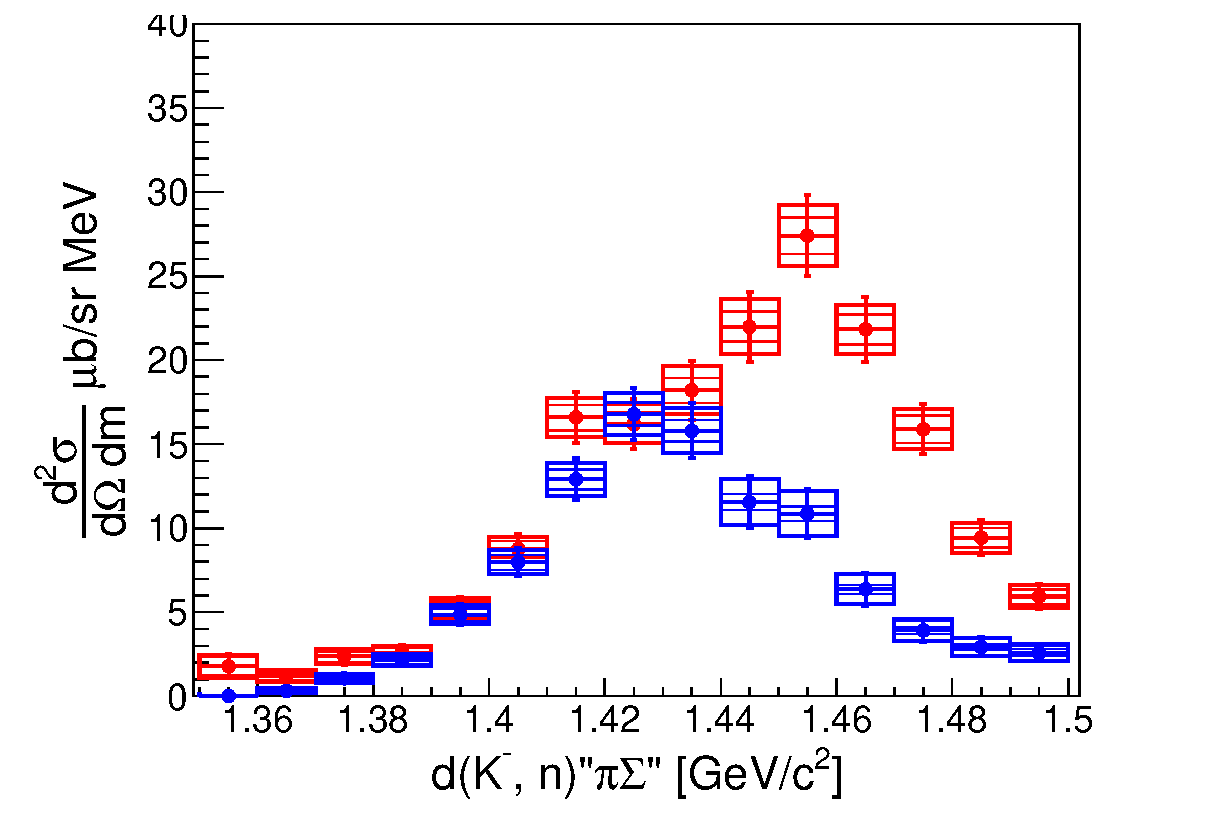
\includegraphics[width=10cm]{fig/tmp.eps}
    \caption{Schematic drawing of the IH.}
    \label{fig-IH}
   \end{center}
  \end{figure}  
\fi  
\subsection{Backward proton detector}
A backward proton detector (BPD) is installed at the most upstream of the CDS to enlarge the acceptance for backward-going charged particles. In particular, it aims to detect a proton from the $\Lambda(1405) \to \Sigma^0\pi^0, \Sigma^0 \to \Lambda\gamma, \Lambda \to p\pi^-$ decay chain in another experiment with the $d(K^-,n)$ reaction (J-PARC E31). 

The BPD is a plastic scintillator hodoscope array with the size of 350 mm (horizontal) $\times$ 340 mm (vertical). It is segmented into 70 units of 5~mm $\times$ 5~mm $\times$ 340~mm scintillation counter made of Eljen EJ-230. Two MPPCs with a 3 mm $\times$ 3 mm sensitive area (Hamamatsu S10362-33-050C) were directly put on both sides of each slab. Signals from the MPPCs are read out by fast timing amps (ORTEC FTA820). 
The BPD is not used in the present analysis except for an energy loss calculation for the kaon beam.

\section{Forward particle detector system}
A forward time of flight (TOF) counter system at 0 degrees with respect to the beam direction, which is installed to detect out-going neutrons and protons in the $^3$He($K^-$, $N$) reactions, is one of the most unique features in our spectrometer system. Flight lengths are kept more than 14 m for both neutrons and protons to achieve good momentum resolution, while keeping acceptance as much as $\sim$20 msr with a large volume of scintillator arrays. The forward TOF counter system is composed of a neutron counter array (NC), a proton counter array (PC) and a charged veto counter array (CVC) as illustrated in Fig. \ref{fig-forward}. The CVC located just upstream of the NC vetoes charged particles injected on the NC, not only detects fast protons. Trajectories of protons are reconstructed with a forward drift chamber 1 (FDC1) installed just downstream the target system, and bended by a dipole magnet named as Ushiwaka towards the PC. At the opposite side of the PC, we constructed a caved beam dump where kaon beams are swept out by Ushiwaka to suppress background events in the neutron spectrum. A beam veto counter (BVC), placed just downstream of the target cryostat, is used to reduce fake triggers for the neutral particle detection.

  \begin{figure}[]
   \begin{center}
    \includegraphics[width=0.9\columnwidth]{illustrator/forward.eps}
    \caption[Schematic view of the forward detectors]{Schematic view of the forward detectors;  the beam veto counter(BVC),  forward drift chamber 1 (FDC1), the beam sweeping magnet, the neutron counter (NC), the charge veto
    counter (CVC), and the proton counter (PC).
    The NC is located 14.7~m away from the final focus
    position.}
    \label{fig-forward}
   \end{center}
  \end{figure}  


\subsection{Neutron time-of-flight counter}
A neutron TOF counter (NC), located 14.7~m away from the final focus point, consists of an array of scintillation counters and has an effective volume of 3.2~m (horizontal) $\times$ 1.5~m (vertical) $\times$ 0.35~m (depth) segmented into 16-column (horizontal) $\times$ 7-layer (depth) units. The acceptance of the neutron counter is $\sim$ 20 msr ; $\pm$ 6.2$^\circ$ in the horizontal direction and $\pm$ 2.9$^\circ$ in the vertical. Each scintillation counter has dimensions of 20~cm (width) $\times$ 150~cm (height) $\times$ 5~cm (thickness) with two 2~inch Hamamatsu H6410 photomultipliers attached to both long sides of the scintillator through a Lucite light guide. The scintillators for the first three layers are made of Saint-Gobain BC408, and the other four layers are made of Saint-Gobain BC412. The average time resolution of the neutron counter, measured with cosmic
rays, is 92 $\pm$ 10~ps ($\sigma$). The error represents the variation among the segments.


\subsection{Charge veto counter}
The charge veto counter (CVC) is located upstream of the neutron counter, 14.0~m away from the final focus point and has an effective area of 3.4~m (horizontal)
$\times$ 1.5~m (vertical) segmented into 34 units. Each scintillation counter has dimensions of 10~cm (width) $\times$ 150~cm (height) $\times$ 3~cm (thickness), and is equipped with two 2~inch Hamamatsu H6410 photomultipliers attached to both long sides of the scintillator through a Lucite light guide. The scintillators are of Eljen EJ-200 type. The average time resolution measured with cosmic rays is 78 $\pm$ 7~ps ($\sigma$). The error represents the variation among the segments.


\subsection{Proton time-of-flight counter}
The proton TOF counter is installed as the extended wall of the charge veto counter. It has an effective area of 2.7~m (horizontal) $\times$ 1.5~m (vertical) segmented into 27 units.
The configuration of each scintillation counter is same with that of the charge veto counter except that a Saint-Gobain BC408 scintillator is used. The average time resolution of the proton counter, obtained from cosmic ray data, is 75 $\pm$ 6~ps ($\sigma$). The error represents the variation among the segments.


\subsection{Beam veto counter}
The beam veto counter (BVC) is attached on the downstream flange of the target cryostat as shown in Fig. \ref{fig:CDS}. The coverage size of the beam veto counter is 320~mm (height) $\times$ 320~mm (width) $\times$ 10~mm (thickness) made of Eljen EJ-200. This size is large enough to cover the acceptance of the neutron counter. The BVC is horizontally segmented into 8 units with different sizes as shown in Fig. \ref{fig-bvc} 
to avoid the over-concentration of the beam on the central segments. 1-inch fine-mesh Hamamatsu R5505 photomultipliers are attached on the both ends of each scintillator segment through Lucite light guides. The signals were read out with an amplification with HOSHIN preamplifier.

  \begin{figure}[]
   \begin{center}
    \includegraphics[width=\columnwidth]{illustrator/BVC.eps}
    \caption{Schematic drawing of the beam veto counter.}
    \label{fig-bvc}
   \end{center}
  \end{figure}  

\subsection{Forward drift chamber}
The forward drift chamber 1 (FDC1) is a feedthrough type chamber which has 6 planes with a VV'XX'UU' configuration. The tilt angles of $U$ and $V$ layers are $\pm$15 degrees. Each layer has 64 sense wires with a drift length of 3 mm which corresponds to an effective area of 384~mm (horizontal) $\times$ 264~mm (vertical). The cell geometry is shown in Fig \ref{fig-bldccell}(c) and the parameters of the chamber are summarized in Table \ref{tab-chamber}. 
The readout method is the same as those for the beam line chambers.

\if0
  \begin{figure}[]
   \begin{center}
    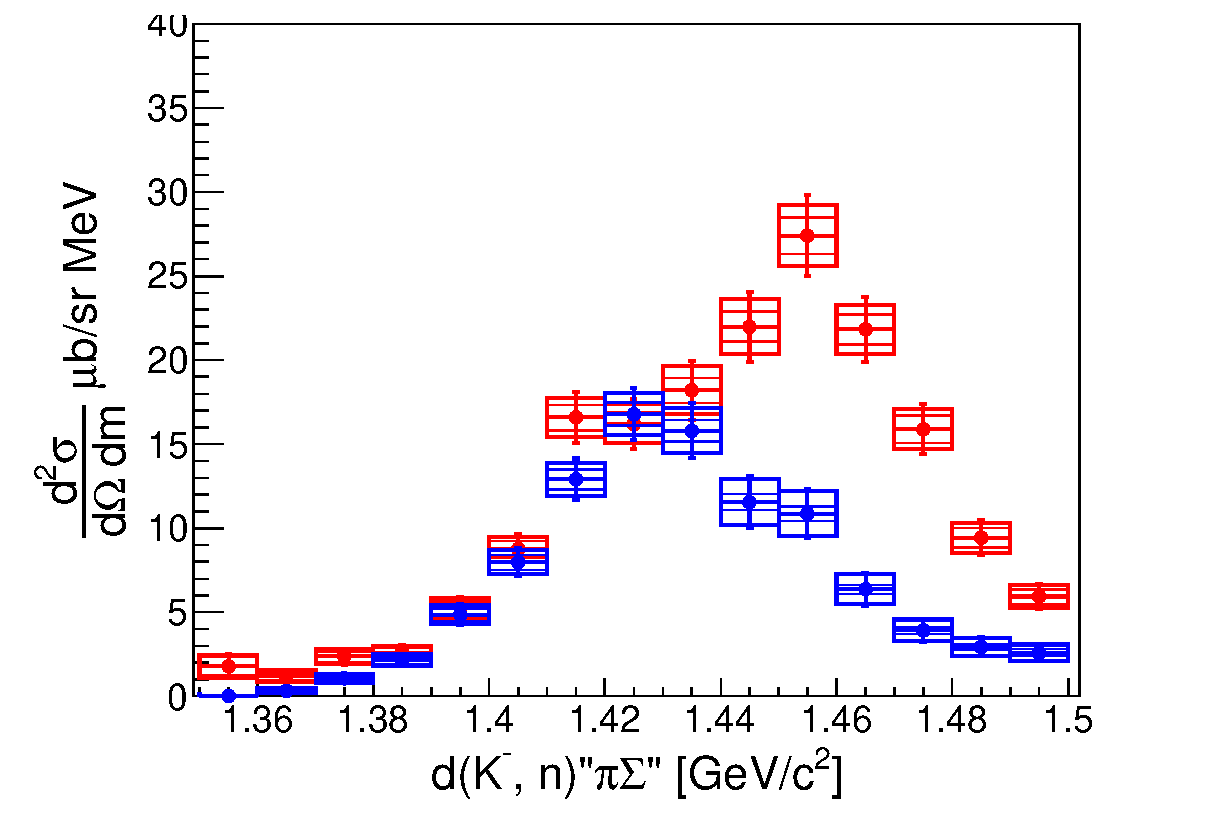
\includegraphics[width=10cm]{fig/tmp.eps}
    \caption{The cell structure of FDC1.}
    \label{fig-fdc1cell}
   \end{center}
  \end{figure}  
\fi

\subsection{Beam sweeping magnet}
A dipole magnet called Ushiwaka %, which was used in the $\pi$2 beam line of the 12 GeV proton synchrotron at KEK, is used as the beam sweeping magnet. It
is located downstream of the CDS and the FDC1 is attached on upstream of the magnet. The magnet has an aperture of 82~cm (horizontal) $\times$ 40~cm (vertical) and a pole length of 70~cm, which accommodates whole acceptance of the neutron counter. Ushiwaka is capable of providing a maximum field of 1.6 T and operated at $\sim$1.0 T in the production run. Figure \ref{fig-dumpprofile} shows the profile at the CVC and the PC with the inverse polarity setting of the Ushiwaka field. We confirmed that the central trajectory of the beam was well apart from the NC (CVC) acceptance, and the contamination in the NC acceptance was less than 3\%.  %Figure \ref{fig-uswkfield} shows a calculated magnetic field along beam axis, from which an effective pole length of 95 mm is obtained at the center of the aperture. 

 \begin{figure}[]
   \begin{center}
    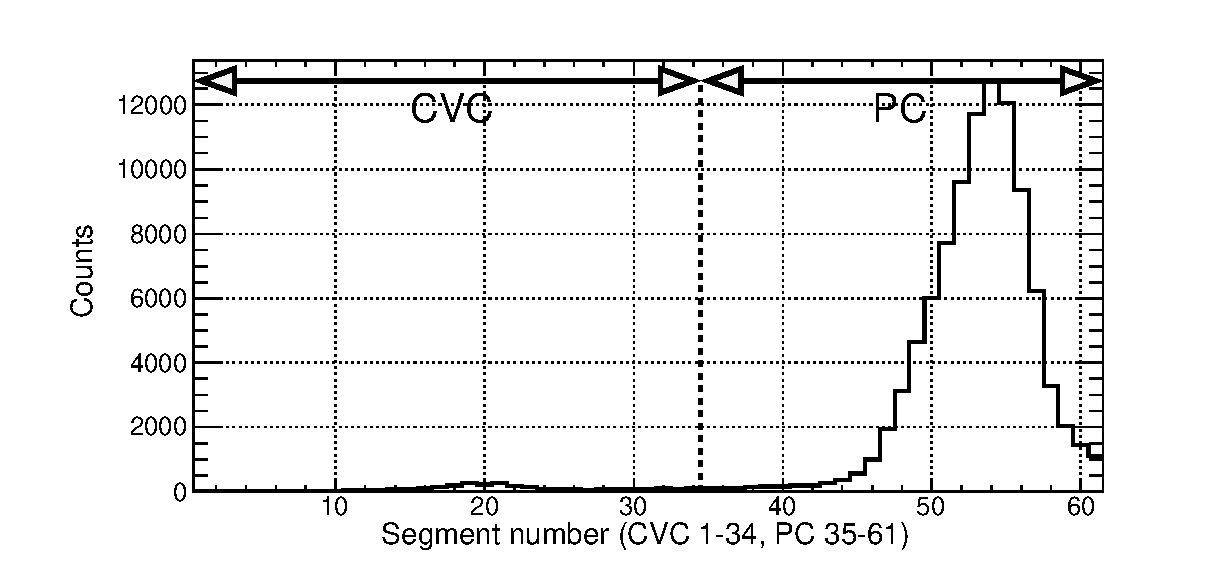
\includegraphics[width=0.9\columnwidth]{fig/dump.eps}
    \caption[Beam profile at the forward counters.]{Beam profile at the forward counters with the inverse polarity setting of the Ushiwaka field. Minimum biased beam data (BHD$\otimes$T0) is analyzed. The bump structure around CVC\#20 is mainly attributed to the pion charge exchange reaction, $\pi^-"p"\to\pi^0n,\ \pi^0\to 2\gamma$.}
    \label{fig-dumpprofile}
   \end{center}
  \end{figure}  

%  \begin{figure}[]
%   \begin{center}
%    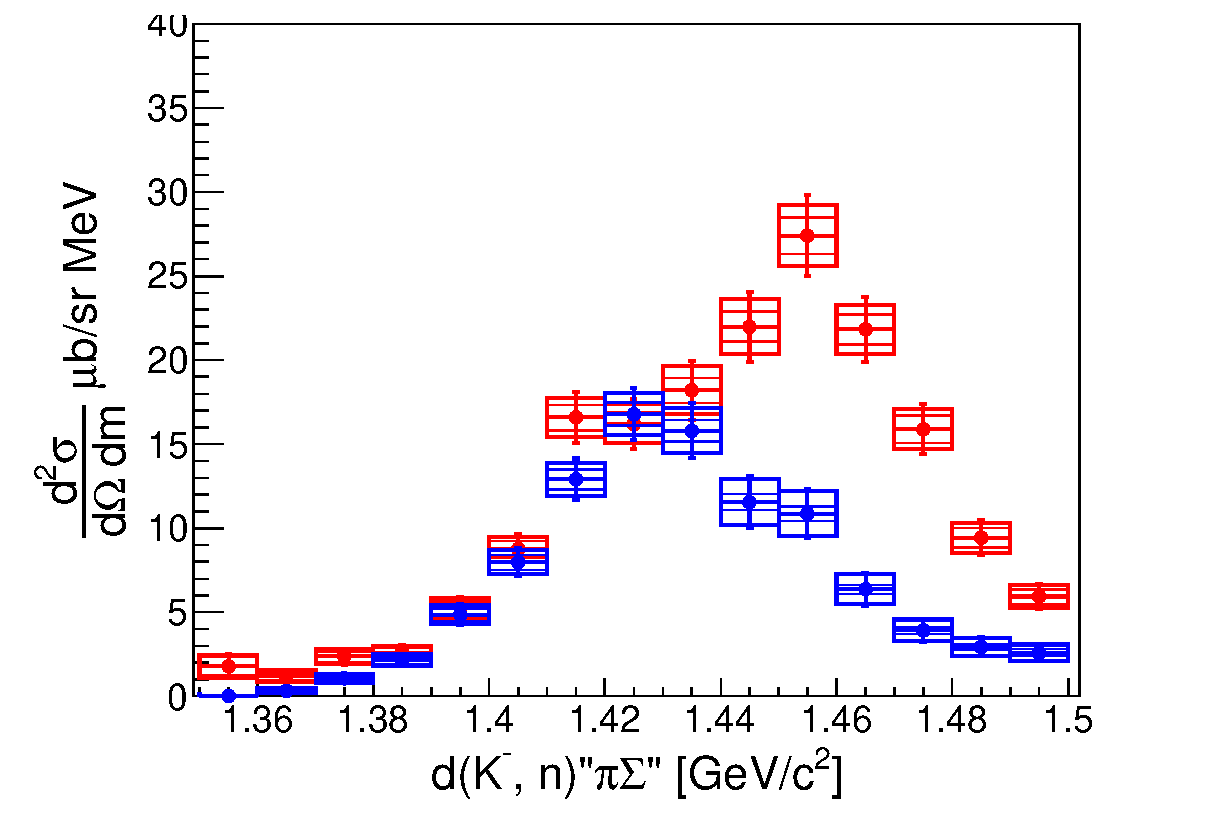
\includegraphics[width=10cm]{fig/tmp.eps}
%    \caption{A calculated field along Z (beam) axis of the Ushiwaka magnet .}
%    \label{fig-uswkfield}
%   \end{center}
%  \end{figure}  

\section{Materials in the spectrometer system}
The materials in the spectrometer system cause the energy losses, the multiple scattering, and the reaction with other than target for the particles. The net effects are expected to result in systematic shifts of the measured momenta, event losses, and additional deteriorations of the spectrometer resolutions. The momenta of the charged particles are corrected particle by particle taking into account the materials on their trajectory. We developed the correction routine for the kaon beam, the charged particles in the CDS and the forward-going charged particles, where the materials summarized in Table \ref{tab-matbeam}, Table \ref{tab-matcdc}, and Table \ref{tab-matforward} were considered, respectively. The wires, the cathode planes and the windows of the chambers, the windows and the reflection sheet of the AC, and the wrapping of the scintillator bars were not taken into account, since their contribution is negligible compared to the required precision of a few MeV$/c$. 

\begin{table}
\begin{center}
\caption[Summary of beam-line materials.]{Summary of beam-line materials between the center of BLC2 ($z$=-130 cm) and the FF. Typical momentum reductions of the kaon and the proton beams at 1 GeV/$c$ are calculated using the Bethe-Bloch formula. }
\label{tab-matbeam}
\begin{tabular}{l|lccccc}
\hline\hline
Component	&	Material	&	Density	&	\multicolumn{2}{c}{Thickness}			&	\multicolumn{2}{c}{$-\delta p$ (MeV/$c$)}				\\
	&		&	g/cm$^3$	&	mm	&	g/cm$^2$	&	1 GeV/$c$ kaon		&	proton	\\
\hline														
BLC2b	&	Ar-isoC$_4$H$_{10}$	&	0.0016	&	100	&	0.02	&	0.03		&	0.07	\\
T0	&	Scintillator	&	1.03	&	10	&	1.03	&	2.4		&	4.2	\\
AC	&	Aerogel	&	0.20	&	100	&	2.00	&	4		&	6.8	\\
BPD	&	Scintillator	&	1.03	&	5	&	0.52	&	1.2		&	2.1	\\
DEF	&	Scintillator	&	1.03	&	3	&	0.31	&	0.72		&	1.2	\\
BPC	&	Ar-isoC$_4$H$_{10}$	&	0.0016	&	60	&	0.01	&	0.02		&	0.03	\\
\hline														
Target system	&		&		&		&		&			&		\\
~~Chamber cap	&	aluminum	&	2.7	&	0.6	&	0.16	&	0.3		&	0.51	\\
~~Radiation shield	&	aluminum	&	2.7	&	0.3	&	0.08	&	0.15		&	0.26	\\
~~Cell cap	&	AlBeMet	&	2.07	&	0.6	&	0.12	&	0.23		&	0.51	\\
~~Target	&	helium-3	&	0.081	&	60	&	0.49	&	1.45		&	2.45	\\
\hline														
Air	&	Air	&	0.0012	&	940	&	0.11	&	0.24		&	0.40	\\
\hline														
Total	&		&		&		&	5.02	&	10.7		&	18.5	\\
\hline\hline						
\end{tabular}
\end{center}
\end{table}


\begin{table}[]
\begin{center}
\caption{Summary of materials used in the energy loss correction of the CDC track.}
\label{tab-matcdc}
\begin{tabular}{l|lccc}
\hline\hline									
Component	&	Material	&	Density	&	\multicolumn{2}{c}{Thickness}	\\
	&		&	g/cm$^3$	&	mm	&	g/cm$^2$	\\
\hline									
Target system	&		&		&		&	0	\\
~~Target	&	helium-3	&	0.081	&	34	&	0.28	\\
~~Cell wall	&	beryllium	&	1.85	&	0.3	&	0.06	\\
~~Radiation shield	&	aluminum	&	2.70	&	0.3	&	0.08	\\
~~CFRP	&	CFRP	&	1.70	&	1	&	0.17	\\
\hline									
Air	&	Air	&	0.0012	&	70	&	0.0084	\\
IH	&	Scintillator	&	1.03	&	3	&	0.31	\\
\hline									
CDC	&		&		&		&		\\
~~CFRP	&	CFRP	&	1.70	&	1	&	0.17	\\
~~Gas	&	Ar-C$_2$H$_6$	&	0.0015	&	380	&	0.057	\\
\hline									
Total	&		&		&		&	1.13	\\
\hline\hline									
\end{tabular}
\end{center}
\end{table}

\begin{table}[]
\begin{center}
\caption[Summary of materials between the FF and the forward counters.]{Summary of materials between the FF and the forward counters. Typical momentum reduction of the proton beam at 1 GeV/$c$ is calculated using the Bethe-Bloch formula. }
\label{tab-matforward}
\begin{tabular}{l|lcccc}
\hline\hline					
Component	&	Material	&	Density	&	\multicolumn{2}{c}{Thickness}	&	$-\delta p$ (MeV/$c$)	\\
	&		&	g/cm$^3$	&	mm	&	g/cm$^2$	&	1 GeV/$c$ proton	\\
\hline											
Target	&		&		&		&		&		\\
~~Target	&	helium-3	&	0.081	&	80	&	0.65	&	3.3	\\
~~Cell cap	&	AlBeMet	&	2.07	&	0.6	&	0.12	&	0.39	\\
~~Rad. shield	&	aluminum	&	2.7	&	0.3	&	0.081	&	0.26	\\
~~Frange	&	SUS304	&	8.9	&	0.3	&	0.27	&	0.26	\\
\hline											
BVC	&	Scintillator	&	1.03	&	10	&	1.03	&	4.2	\\
FDC1	&	Ar-C$_6$H$_{10}$	&	0.0016	&	100	&	0.016	&	0.053	\\
\hline\hline											
to PC	&		&		&		&		&		\\
~~Air	&	Air	&	0.0012	&	1.3E+04	&	1.57	&	5.2	\\
\hline											
~~Total	&		&		&		&	3.71	&	13.6	\\
\hline\hline											
to NC	&		&		&		&		&		\\
~~Air	&	Air	&	0.0012	&	1.4E+04	&	1.69	&		\\
~~CVC	&	Scintillator	&	1.03	&	30	&	3.09	&		\\
\hline											
~~Total	&		&		&		&	6.92	&		\\
\hline\hline									
\end{tabular}
\end{center}
\end{table}

\section{Data acquisition}
\subsection{Data acquisition system}
The on-line data acquisition system (DAQ) consists of the TKO\cite{Ohska:1986gf,Group:1985tn}, VME, and PC Linux.
The signals from the detectors are fed into ADC and TDC modules slotted into 10 TKO crates.
They are read in parallel with 10 VME-SMPs (super memory partner\cite{Shiozawa:1994ja}) via a TKO SCH (super
controller head). The data stored in a buffer memory of the SMP is transferred to the DAQ-PC through SBS Bit3 VME-to-PCI bridges.
Additionally, two DAQ systems consist of VME and PC Linux are used. One is for spill by spill readout of scalers, and the other one is for multi-hit TDC readout for beam-line counters. To secure event matching in the offline analysis, an event and a spill numbers are distributed the three DAQ systems by using a master trigger module and receiver modules and event matching is done offline.
The status of the detector system, such as temperature of the cryogenic target system and the magnetic field of the D5 magnet  was recorded by using LabVIEW based program.

Since current DAQ system has no buffer memory in TDC and ADC modules, the fast clear scheme is adopted to efficiently accumulate the ($K^-,N$) events. The $1^{st}$ level trigger is constructed by the beam line detectors and CDS, and then TDC common start/stop signals and ADC timing gates are distributed to each module, followed by analog-to-digital conversion. Signals of the forward counters reach the DAQ system 100 ns or more after $1^{st}$ level decision. Then $2^{nd}$ level trigger is generated by the forward-counter signals. If $2^{nd}$ level is not acceptable, the analog-to-digital conversion is suspended and the modules are initialized for the next event ($Fast Clear$).

The dead time of conversion in ADC/TDC and data-transfer from TKO-SCH to VME-SMP is $\sim$ 120 $\mu$s and $\sim$ 230 $\mu$s. respectively. The dead time caused by a data-transfer from VME-SMP to the PC-Linux is negligible by using two buffers in the VME-SMP. In the case of $Fast Clear$, it takes only $\sim$3 $\mu$s to be ready for the next event. During the main data taking period, a typical DAQ rate was about 800 events per spill with the live rate of $\sim$81\%.

\subsection{Trigger scheme}
We constructed a trigger scheme to satisfy the requirement to derive physical quantity out of the data. Table \ref{tab-trigger} shows a list of trigger mode in the production run. %These triggers are constructed from the first level triggers and the second level triggers listed in Table \ref{tab-trig2}.
The trigger logic diagram is shown in Fig. \ref{fig-trig}.
\subsubsection{Kaon beam trigger}
The elementary beam trigger is constructed by coincidence signals from the beam line counters, the BHD, T0 and the DEF. The kaon beam trigger $(K_{\rm beam})$ is selected from the beam trigger by using the kaon identification counter, i.e., a veto signal of the AC ($\overline{\rm AC}$) defines the kaon beam. It should be noted that antiprotons in the beam are eliminated upstream of the beam line by using the ES1, CM1, and CM2.
	    A logical expression of the kaon beam trigger is given as 
	    \begin{eqnarray} 
	     \nonumber
	      (K_{\rm beam}) \equiv ({\rm BHD}) \otimes ({\rm T0}) \otimes ({\rm DEF})
	      \otimes (\overline{\rm AC}).
	    \end{eqnarray}
A pion beam trigger requires coincidence signal of AC. Then,
	    \begin{eqnarray} 
	     \nonumber
	      (\pi_{\rm beam}) \equiv ({\rm BHD}) \otimes ({\rm T0}) \otimes ({\rm DEF})
	      \otimes ({\rm AC}).
	    \end{eqnarray}

 \subsubsection{Main trigger}
 A two-level trigger logic for the in-flight $^3$He$(K^-, N$) reaction is applied. To reconstruct the reaction vertex by using the CDS, events with one or more CDH hits (${\rm CDH}^{1hit}$) are selected from the kaon beam trigger in the first level. In addition, a forward neutral trigger (Neutral) or a forward charged trigger (Charged) are required in the second level. The neutral trigger is composed of one or more hits on the neutron counter ($\rm NC$) and a veto signal of the charge veto counter ($\overline{\rm CVC}$). The forward charged trigger requires one or more hits on the charge veto counter and/or the proton counter. 
The E15 main trigger is given as
\begin{eqnarray} 	
      (\rm{Main}) &\equiv& (K_{\rm beam}) \otimes ({\rm CDH}^{1hit})   \otimes \left( ({\rm Neutral}) \cup  ({\rm Charged}) \right), \nonumber
\end{eqnarray}
where, 
\begin{eqnarray} 
     	({\rm Charged}) &\equiv& ({\rm CVC}) \cup ({\rm PC})   \nonumber \\
     	({\rm Neutral}) &\equiv& ({\rm NC}) \otimes (\overline{\rm CVC}).   \nonumber
\end{eqnarray} 

\subsubsection{Triggers for the neutron counter calibration}
A time offset calibration is of vital importance to precisely measure momenta of the forward-going nucleons by TOF method. To calibrate the NC run by run, gamma-rays from the target are accumulated in addition to the main trigger. Note that although gamma-ray events are contaminated in the main trigger, it is not enough for the calibration purpose.
Then, two triggers are introduced which are given as,
\begin{eqnarray} 
 (\pi_{beam})\otimes(\overline{\rm{BVC}})\otimes(\rm{Neutral}) \nonumber \\
 (K_{beam})\otimes(\overline{\rm{BVC}})\otimes(\rm{Neutral}) \nonumber ,
 \end{eqnarray} 
where the (Neutral) trigger is the second level one. 

\subsubsection{Triggers for normalization}
For the evaluation of reaction cross sections, the total kaon flux on the target is crucial. Therefore, elementary kaon beam data ($K_{beam}$) is also recorded. Minimum-biased beam data (BHD$\otimes$T0) is also mixed to monitor the performance of the AC and the DEF.

\subsubsection{$K_{beam}$$\otimes$CDH triggers} 
Since the main trigger rate is few hundreds per spill, the DAQ has still room to take additional data. Although primary purpose of the present experiment is the study with forward-going nucleons, some physical output without forward counters are also expected. Among them, the $\Lambda p$ events in the CDS are most interested in. Therefore, kaon beam triggers with the coincidence of the CDH hit(s) are mixed as much as possible to keep DAQ live rate better than 80\%.

\subsubsection{Cosmic trigger}
A cosmic data triggered by two or more CDH hits were recorded to monitor the CDS performance between the spills.

 \begin{table}[]
  \begin{center}
   \caption{Summary of trigger conditions.}
   \label{tab-trigger}
   \begin{tabular}{l|cccl}
\hline\hline									
	&	\shortstack{request\\ / spill}	&	\shortstack{pre-scale\\ factor}	&	\shortstack{accept\\/ spill}	&	main usage	\\
\hline									
BHD$\otimes$T0	&	610k	&	50k	&	10	&	monitor AC\&DEF	\\
$K_{beam}$	&	145k	&	7k	&	17	&	normarisation	\\
$K_{beam}\otimes$CDH$^{1hit}$	&	48k	&	70	&	70	&		\\
$K_{beam}\otimes$CDH$^{2hit}$	&	21k	&	7	&	280	&	$\Lambda p$ events	\\
$K_{beam}\otimes$CDH$^{1hit}\otimes$Neutral	&	230	&	1	&	170	&	($K^-,n$)	\\
$K_{beam}\otimes$CDH$^{1hit}\otimes$Charged	&	130	&	1	&	100	&	($K^-,p$)	\\
$\pi_{beam}\otimes\overline{\rm{BVC}}\otimes$Neutral	&	480	&	10	&	40	&	NC calibration	\\
$K_{beam}\otimes\overline{\rm{BVC}}\otimes$Neutral	&	850	&	10	&	70	&		\\
\hline									
Total	&	8.5k	&		&	680	&	($1^{st}$ accept $\sim$ 6.9k)	\\
\hline\hline									
\end{tabular}
  \end{center}
 \end{table}
\subsection{Trigger efficiency \label{sec-trigeff}}
In the data analysis, the $K_{beam}$ trigger data was the minimum-biased one to evaluate the number of incident kaons. Then, the trigger efficiency of the main trigger, $(K_{\rm beam}) \otimes ({\rm CDH}^{1hit}) \otimes \left( ({\rm Neutral}) \cup ({\rm Charged}) \right)$, was evaluated in two steps. The $({\rm CDH}^{1hit})$ trigger efficiency was evaluated first using the $K_{beam}$ data. The $({\rm CDH}^{1hit})$ trigger was reconstructed in the offline analysis and then checked the $(K_{\rm beam}) \otimes ({\rm CDH}^{1hit})$ trigger flag. The efficiency was evaluated to be (98.6 $\pm$ 0.1)\%, where the statistical one. The systematic error in the offline coincidence gate of the CDH signal with the kaon beam was evaluated to be negligibly small. Then the (Neutral)$\cup$(Charged) trigger efficiency was evaluated in a similar way to be (99.83 $\pm$ 0.01)\% with the $(K_{\rm beam}) \otimes ({\rm CDH}^{1hit})$ trigger data. The efficiency of the main trigger was obtained as the multiple of the two efficiency to be (98.3 $\pm$ 0.1)\%.

Note that the present trigger condition generates the $2^{nd}$ level trigger by any signals from the forward counters, the NC, the CVC, and the PC, since the pre-scale factors of the (Neutral) and the (Charged) triggers were 1. In the analysis, we did not distinguish the two $2^{nd}$ level triggers, and performed the same analysis procedure as described in Sec. \ref{sec-ananc}. 

\subsection{DAQ live rate \label{sec-daqrate}}
The DAQ live rate can be obtained as the ratio of the number of accepted $1^{st}$ level triggers to that of requested ones. Typical numbers per spill of the accepted $1^{st}$ level triggers and the $1^{st}$ level requests are $\sim$8500 and $\sim$ 6900, respectively. Considering the fluctuation in the experimental period as the error, the DAQ live rate was obtained to be (81.5 $\pm$ 0.7)\% at the data acquisition rate of $\sim$680 events per spill.

\subsection{Data summary}
The production of present experiment was carried out from May 18th, 2013 to May 23rd, 2013, after a short period of beam-tuning and separated calibration runs. The calibration runs contained target empty runs for the fiducial volume study, proton beam through runs to calibrate the beam absolute momentum and pion beam runs for chamber position calibrations and ADC calibrations. The field of the Ushiwaka was scanned in the dedicated run to irradiate pions on the all segments of the NC and the PC.

The total primary beam amount we received in the physics run was $\sim$12 kW$\times$week. The integrated number of kaons evaluated by scaler count of the kaon trigger was 7.52 $\times 10^9$, $\sim$70\% of which were focused on the $^3$He target. %A summary of data acquisition in data used in the current analysis is tabulated in Table \ref{tab-data}.

\begin{landscape}
  \begin{figure}[]
   \begin{center}
    \includegraphics[width=\columnwidth]{fig/trigger_for_dth.eps}
    \caption{Logic diagram of the trigger circuit.}
    \label{fig-trig}
   \end{center}
  \end{figure}  
\end{landscape}


\chapter{Data analysis}
%\chapter{Detector analysis}
\section{Overview}
This chapter is dedicated for the data analysis to obtain the missing mass spectra in the $^3$He($K^-, n$) reaction. 

The first part of this chapter describes analyses of individual detectors. First, common procedures for all the counters are described in Sec. 3.2. Then, an analysis of the kaon beam is presented and the selection of the kaon beam is defined in Sec. 3.3. The analysis of the cylindrical detector system (CDS) comes to the next. A tracking method of the cylindrical drift chamber (CDC) is presented to reconstruct a reaction vertex, and a particle identification is performed to reconstruct $K^0_s$ and $\Lambda$ peaks for the performance check in Sec. 3.4. An analysis of the forward neutron appears in Sec. 3.5. 

In the later part of this chapter, an analysis with a whole system is presented. The resolution and the precision of scale in the $^3$He($K^-,n$) missing mass are evaluated in Sec.~3.6 and Sec.~3.7, respectively. Finally in Sec. 3.8, the normalization factors of the missing mass spectrum is evaluated including the neutron detection efficiency with the NC.

\subsection{Definition of the coordinates}
In the present analysis, we employ the right-handed system, where $z$-axis is defined by the (designed) beam-axis, and then $x-$ and $y$-axis represent horizontal and vertical positions, respectively. A positive $x$ position corresponds to right-hand side from the beam axis when we look from downstream of the beam line.
\section{Common procedures to all detectors}
\subsection{TDC data conversion to the time}
To convert a TDC channel to time, conversion parameters, i.e., the time gain, were obtained channel by channel with a time calibrator (ORTEC 462). The calibration data were recorded before the experiment. We used linear functions for the wire chambers and quadratic curves for the scintillation counters to describe conversion parameters of their TDCs.% A measured integral non-linearity of a TDC channel for a segment of the neutron counter is shown in Fig.\ref{}, together with the time difference between the measurement and estimation with a quadratic conversion curve.

\subsection{ADC data conversion to the energy}
For the conversion from an ADC channel to energy, 1 GeV/$c$ $\pi^-$ beams, whose energy deposit on a scintillator is $\sim 2$ MeV/1 cm, is used. To calibrate ADCs of the forward counters, we took a dedicated run to irradiate the pion beam to all the segments by scanning the Ushiwaka field before the experiment and once during the experiment. For the ADCs of the CDH and the IH, reconstructed pion tracks with the CDC were used as the calibration source, considering their track length in the scintillator event by event. 

\subsection{Time-walk correction and time offset tune for scintillation counters.}
The time-walk effect is well-known phenomenon that the timing signal generated by a threshold-type discriminator has systematic dependency on the pulse height or the charge of the raw signal. The effect was compensated at offline analysis with a correction function,
\begin{eqnarray*}
p_0+\frac{p_1}{\sqrt{dE}}+p_2\cdot dE
\end{eqnarray*}
where $dE$ is the energy deposit on the photo-sensor recorded with an ADC, $p_i$ are the parameters. These parameters were obtained by iteratively correcting the $dE$-timing relation with well defined velocity particles such as $\pi$ beam and $\gamma$-rays. The timing offsets were also adjusted in this procedure by optimizing the parameter $p_0$ run by run.

\subsection{Hit timing determination of a hodoscope segment}
A particle hit on a hodoscope segment was identified by the coincidence of the TDC signals of all photomultipliers; one for the IH, and two for the other detectors. The timing was determined by the mean of the TDC timings after the time-walk correction.
\section{Kaon beam analysis\label{sec-anabeam}}
In the kaon beam analysis, we identified true kaons in the kaon triggered events and obtained their momenta and trajectories. One of the most important point of the beam analysis is to assure only one beam particle is coming into the spectrometer during the time range we are interested in. Otherwise, we can not distinguish (from which beam particles a forward-going particle is generated, especially when it is neutral. %Furthermore, as already mentioned in Sec \ref{},
Furthermore, the kaon beam has microscopic beam structure which may cause fake peak structures in the $^3$He($K^-,n$) spectrum. In the current analysis, we set a time gate of forward-going particles to be the same as the TDC range of T0, $\sim$100 ns. It corresponds to down to $\sim$ 400 MeV/$c$ neutrons. To cover this time range, we selected single beam events between -30 ns and 100 ns.% with respect to a triggered particle.

An analysis procedure of the kaon beam is:
\begin{enumerate}
\item Select T0 single hit event.
\item Require that the TOF between T0 and the BHD is consistent with that of kaon beam.
\item Require that the BPC has only one track.
\item Require that BLC1 and BLC2 have only one track each.
\item Reconstruct beam momentum and check consistency with BHD hit.
\item Check consistency between BLC2 and BPC tracks.
\item Require that an extrapolation of the BPC track is on the target fiducial volume.
\end{enumerate}
The details of each step are described below.
\subsection{Kaon identification by the TOF between the BHD and T0}
Although the kaon beam is identified at the online trigger level with the AC, there are still small contaminations of pions due to the inefficiency of the AC. In addition, many events have multiple hits on the BHD and T0 as shown in Fig. \ref{fig-mulbhdt0}. We first selected T0 single-hit events to avoid beam pile-up, while we allowed multiple hits on the BHD since otherwise more than half of the statistics was lost. Instead, we developed a timing analysis method for the beam line drift chambers as described in the next section and rejected the beam pile-up event at downstream of the D4 magnet.

The associated BHD hit to the T0 hit was selected by requesting the time-of-flight between BHD and T0 to be consistent with the 1 GeV/$c$. The relative time offset and time-walk effect of the BHD was calibrated with respect to T0 segment \#3 by using pions with a fixed flight length of 7.7 m and a fixed beam momentum of 1 GeV/$c$. A typical TOF resolution of 160 ps ($\sigma$) was obtained for 1 GeV/$c$ pions, where the flight length deviation from the central trajectory is not taken into account. A typical TOF spectrum is shown in Fig. \ref{fig-tofk}. The kaon selection gate was defined by the 3$\sigma$ of the kaon peak, where the TOF resolution for 1 GeV/$c$ was evaluated to be 195 ps($\sigma$). The additional deterioration of the resolution is due to the ignorance of the $\sim$ 2\% beam momentum bite.
\begin{figure}[]
\begin{center}
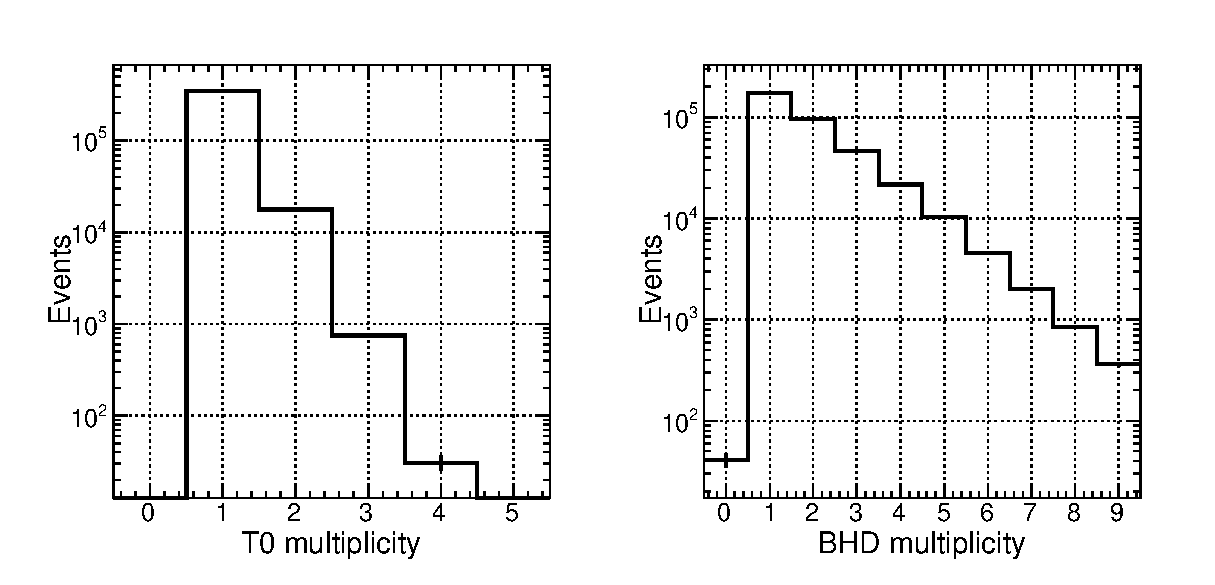
\includegraphics[width=\columnwidth]{./fig/mul-bhdt0.eps}
\caption[Multiplicity of T0 and the BHD.]{Multiplicity of (left) T0 and (right) the BHD for the unbiased-kaon beam. The T0 single-hit is required in the right figure.}
\label{fig-mulbhdt0}
\end{center}
\end{figure}  
\begin{figure}[]
\begin{center}
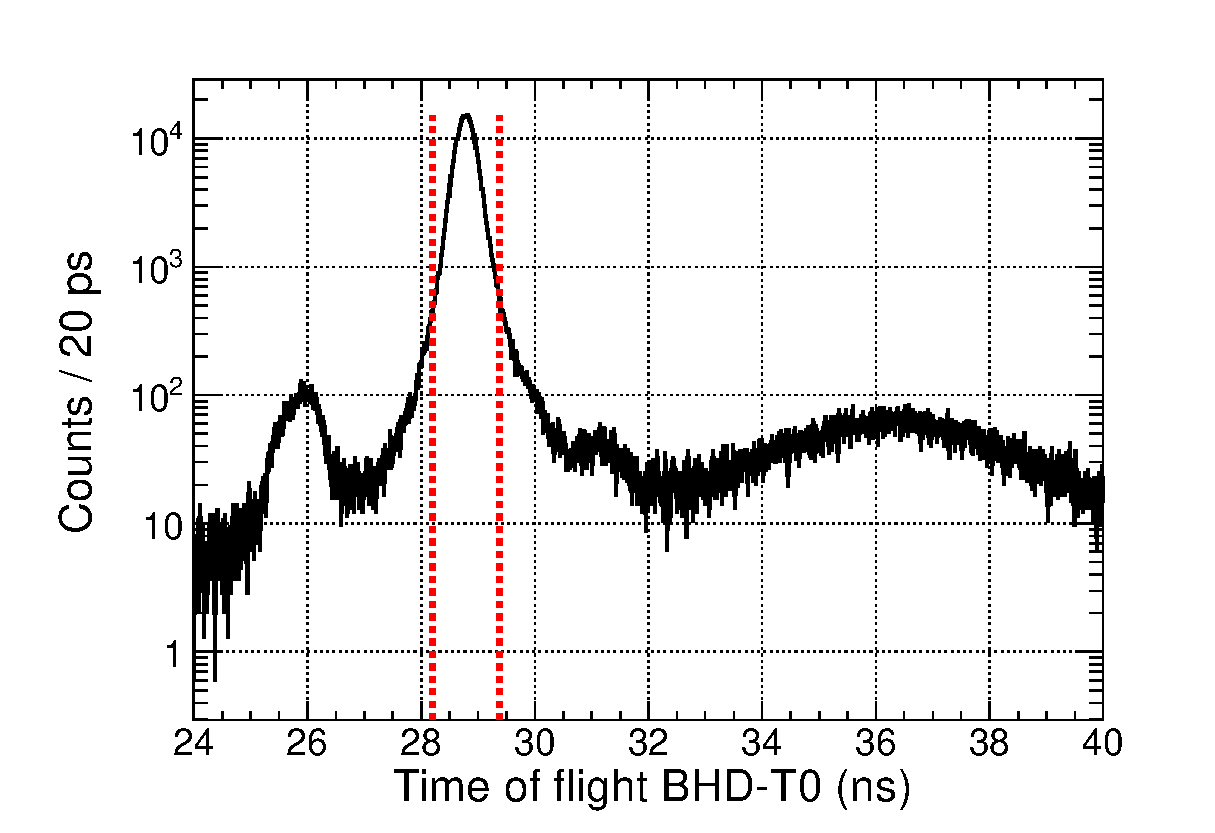
\includegraphics[width=10cm]{./fig/tofk.eps}
\caption[Time-of-flight distribution between the BHD and T0.]{Time-of-flight distribution between the BHD and T0. Unbiased kaon trigger data is used. Multiple hits on the BHD are allowed. A peak around 29 ns corresponds to the kaon timing and the red dot lines show the kaon selection region. A peak around 26 ns is contributed from pion contamination. A bump above 33 ns is considered due to the beam pile-up events.}
\label{fig-tofk}
\end{center}
\end{figure}  
\subsection{Beam-line drift chamber analysis}

\subsubsection{Conversion to the hit position}
The TDC data of drift chambers is converted to drift time information. Assuming that the beam particles pass through the chambers at right angles and are uniformly distributed in each cell, a conversion relation between a drift time and a drift length can be obtained from the integral of the time distribution as shown in Fig. \ref{fig-bldcdtdx}(top and middle). The conversion relations were obtained wire by wire with the kaon beam, and a relative offset of each wire was adjusted by using a peak position in the differentiated time spectrum as shown in Fig.~\ref{fig-bldcdtdx}(bottom).

\begin{figure}[]
\begin{center}
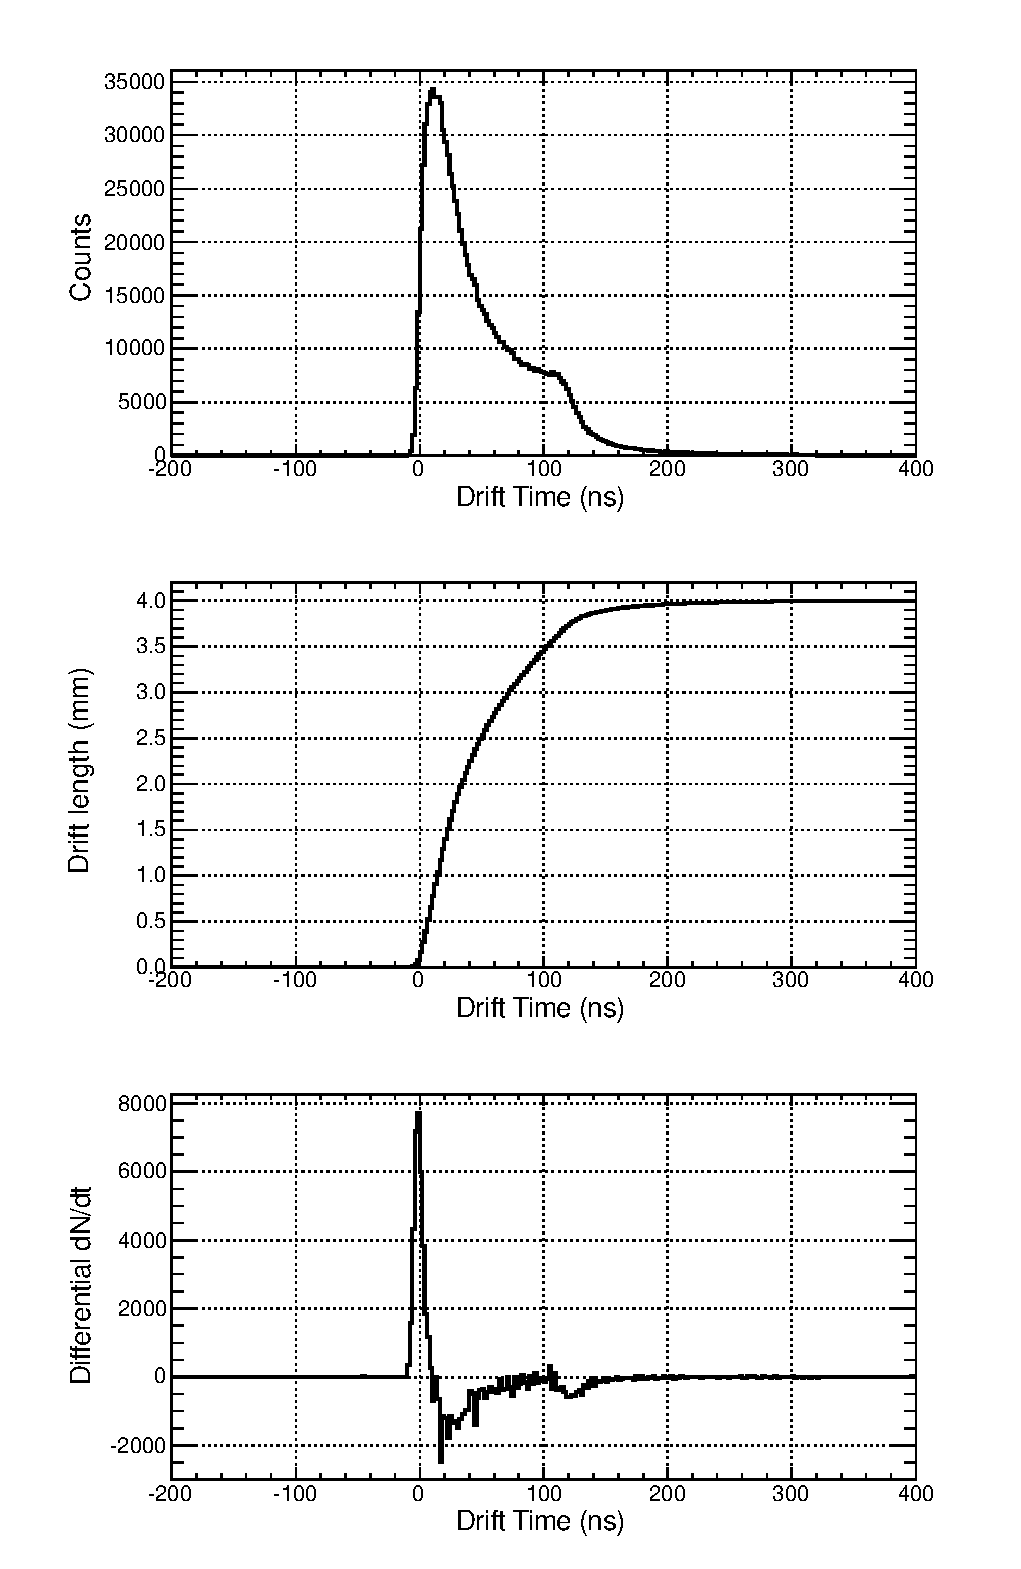
\includegraphics[width=12cm]{./fig/bldcdtdx.eps}
\caption[Timing distribution, integrated timing spectrum, and differential timing spectrum of a typical wire in BLC1.]{(top) Timing distribution of a typical wire in BLC1. (middle) Integrated timing spectrum. The maximum was normalized by the maximum drift length. (bottom) Differential of the timing distribution. The peak position was used to adjust the relative timing offset.}
\label{fig-bldcdtdx}
\end{center}
\end{figure}  

\subsubsection{Linear tracking}
A hit position in each plane can be calculated from a wire position and a drift length, but there is still ambiguity in the drift direction. For a given set of the hits, all combinations of the drift directions were examined and the combination which gives minimum $\chi^2/ndf$ was selected. The $\chi^2/ndf$ in the 3 dimensional linear fitting is defined as,
\begin{eqnarray}
\chi^2/ndf&=& \frac{1}{N-4}\sum_i^N\left(\frac{x'_i-f(z_i)}{\sigma_i}\right)^2,\\
f(z)&=& \cos\theta(a+zb)+\sin\theta(c+zd), \label{eq-trackrot}
\end{eqnarray}
where $N$ is the number of the given hits, $x'$ is the positions perpendicular to the wire and the beam direction,  $f(z)$ is the calculated position in a rotated plane with an angle of $\theta$, and $\sigma$ is the assumed position resolution. We employed the position resolutions in Table \ref{tab-chmperformance} for the calculation. The four parameters a, b, c, d in eq. \ref{eq-trackrot} at the minimum $\chi^2$ are analytically calculated for the given set of the hits.

\subsubsection{Timing analysis}
Since the gate windows for the TDCs were set to $\sim$500 ns, there were many multi-track events which had multi hits in the beam line drift chambers. To select a correct set of the hits and to reject tracks out of the triggers particle, a timing analysis was introduced. Although a single-hit-timing information is useless due to large drift-time distribution of $\sim$100 ns, the timing of the particle passage can be deduced by using hits of paired plane, such as $XX'$.

All beam-line chambers  consist of pairs of staggered planes by a half of the cell size. Therefore, for the correct set of the hits,  a sum of the drift lengths of the paired hits should be approximately the cell width, i.e., the drift times in the paired planes should be correlated. Figure \ref{fig-dctime}(top) shows the relation between a differential and an average of drift times in the paired planes. Here, single-track events were selected to ensure the hits were generated by the trigger particle. The correlation in Fig. \ref{fig-dctime}(top) is due to the asymmetric conversion relation between the drift time and the drift length (Fig, \ref{fig-bldcdtdx}(middle)). After correcting the correlation as shown in Fig. \ref{fig-dctime}(b), the corrected average drift-time gives the timing of the particle passage. The correction relations were determined plane by plane. Note that when the paired-hits search was failed, then those paired planers were excluded from the timing analysis.

\begin{figure}[]
\begin{center}
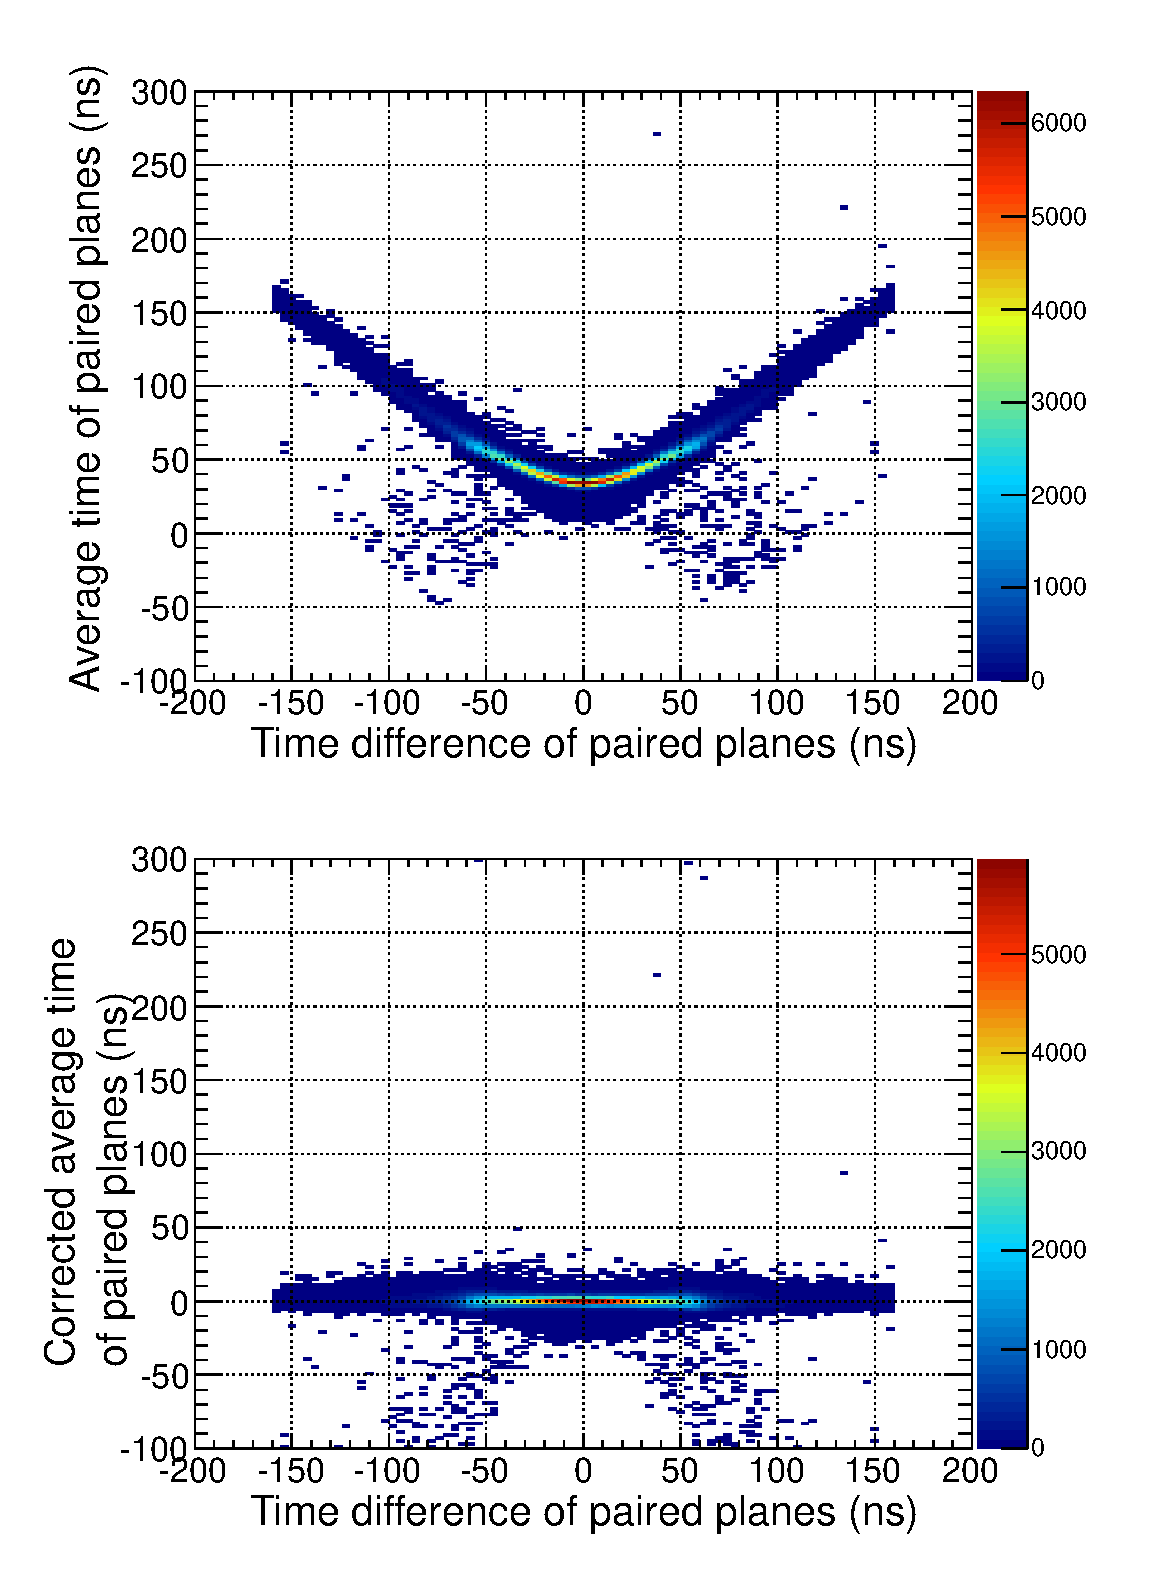
\includegraphics[width=12cm]{./fig/dctime.eps}
\caption[Typical correlation of the time difference and the average time of paired plane.]{(top) Typical correlation of the time difference and the average time of two neighboring wire hits. Single track event at 0 ns is selected with other chambers and counters. (bottom) After the correction. }
\label{fig-dctime}
\end{center}
\end{figure}  

\subsubsection{Track search at a local level}
At first, tracks were searched at a local level, BLC1, BLC2 and the BPC, independently. All possible candidates of hit combinations were examined. For BLC1 and BLC2, a candidate was required to have hits in more than 5 planes out of 8 planes in each of U and V planes. All 8 planes were requested to have hits for the BPC because of the lack of redundancy. The number of candidates was reduced with the help of timing analysis and pre-fitting with a MWPC mode, namely without drift time consideration. Then a hit combination with a minimum $\chi^2/ndf$ was selected as a first track. The procedure was iteratively done with hits not included in reconstructed tracks, until we have no more hits enough to reconstruct an additional track. 

\subsubsection{Definition of a good track}
The reconstructed tracks were further examined. First, the $\chi^2/ndf$, whose typical distributions are shown in Fig. \ref{fig-bldcchi}, was requested to be less than 10. To avoid beam pile-up events, single track event within the timing window of (-30,100) ns was selected as shown in Fig.\ref{fig-bldctime}. In addition, the tracks were also required to be associated to the trigger timing. The timing windows of the trigger association were defined to be (-5,5) ns and (-10,10) ns for the BLCs and the BPC, respectively. Typical track multiplicities are shown in the right of Fig. \ref{fig-bldctime} for different timing windows.

\begin{figure}[]
\begin{center}
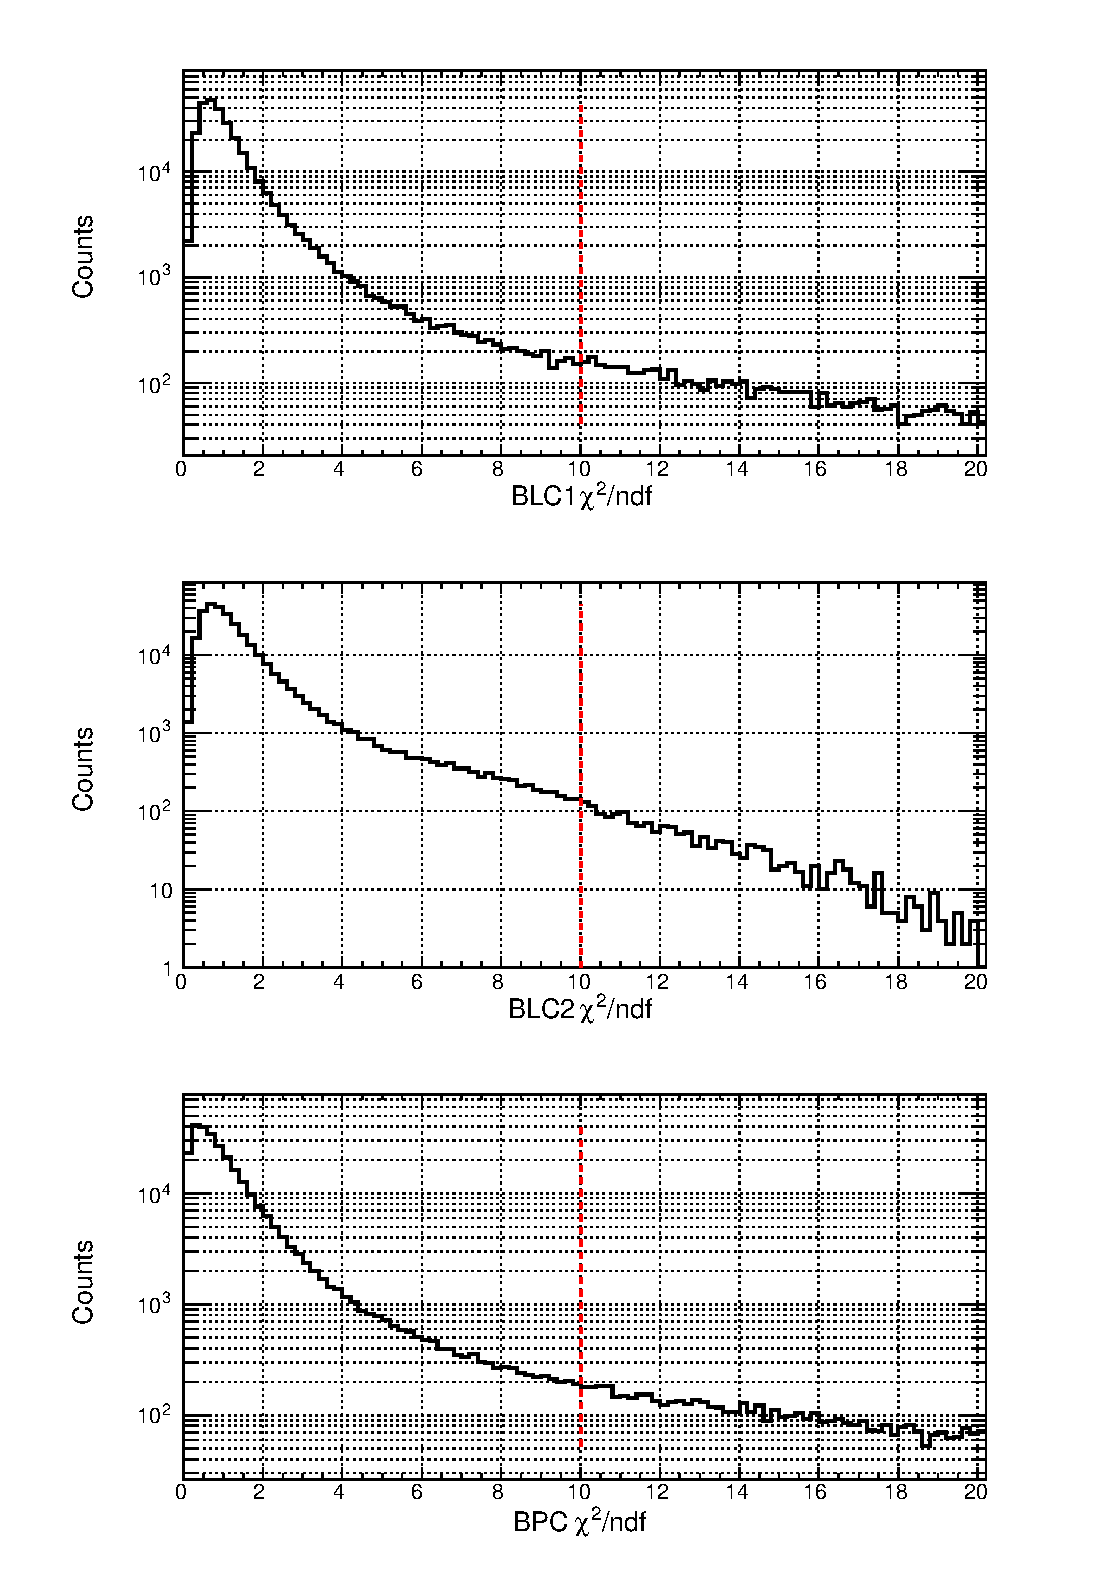
\includegraphics[width=12cm]{./fig/bldc-chi2.eps}
\caption[$\chi^2/ndf$ distributions of BLC1, BLC2 and the BPC. ]{$\chi^2/ndf$ distributions of BLC1, BLC2 and the BPC. $\chi^2/ndf<$10 tracks were accepted. }
\label{fig-bldcchi}
\end{center}
\end{figure}  

\begin{figure}[]
\begin{center}
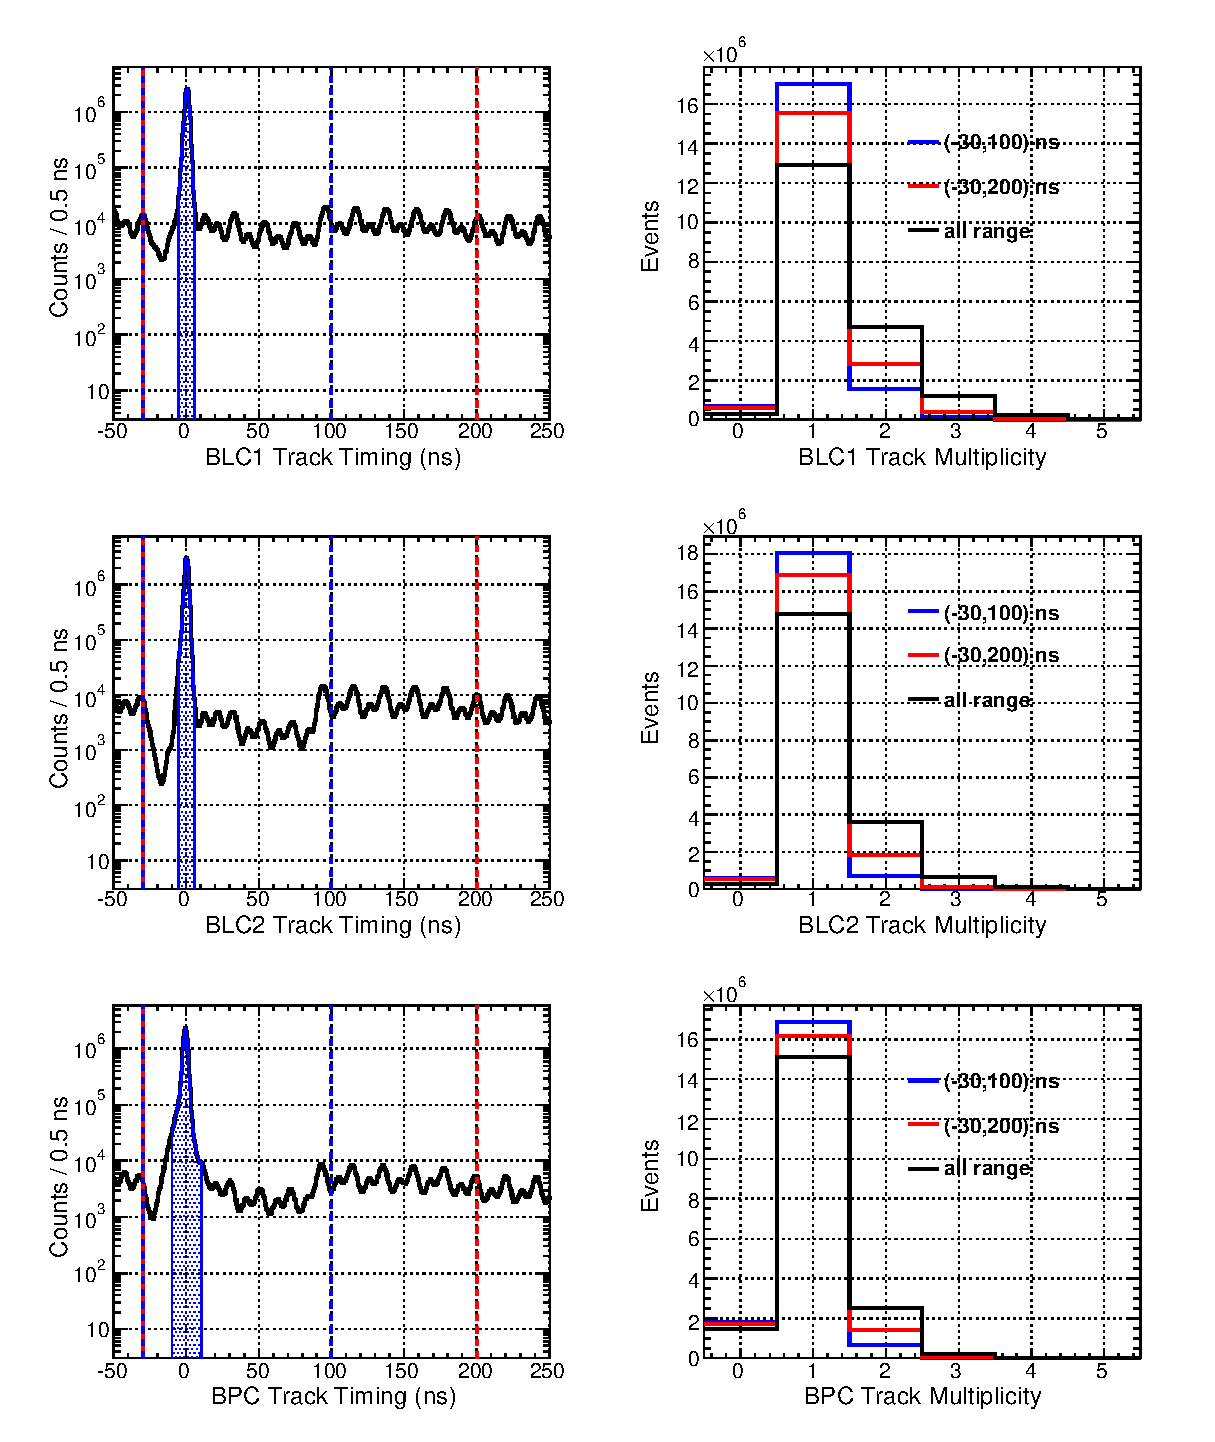
\includegraphics[width=14cm]{./fig/chmtime.eps}
\caption[Track timing distributions and track multiplicities of the beam-line drift chambers.]{(left) Track timing distributions. T0 single hit and at least 1 CDC track were already required. Due to the T0 single hit selection, pile-up events in the T0 TDC range of (-20, 80) ns was reduced. The largest peak around 0 ns corresponds to the triggered particle and others are pileup events. The red dotted lines give the region for the multiplicity counting and the trigger associated windows were defined as blue hatches. (right) Track multiplicities with different timing windows. The (-30,100) ns timing window is employed in the current analysis.}
\label{fig-bldctime}
\end{center}
\end{figure}  

%\end{enumerate}
\subsection{Performance of the beam line drift chambers}
\subsubsection{Position resolution}
An intrinsic position resolution of the plane is related to the residual distribution. The residual distribution for all wires in the plane was fitted with a Gaussian and the resultant Gaussian sigma is converted to the intrinsic position resolution by using a factor calculated with the geometry of the chamber.  Typical resolutions appear in Table \ref{tab-chmperformance} are averages of the resolutions of all planes in the drift chambers.  
%The time dependency of the same quantity is plotted in Fig. \ref{} for BLC1, BLC2 and BPC.
\subsubsection{Timing resolution}
Since the typical drift velocity under the present operational condition is $\sim$ 50 $\mu$m/ns, the timing resolutions in the paired plane analysis are expected to be a few ns. The time resolution of a paired planes were obtained to be $\sim$ 3 ns from the Y-projected distribution of Fig. \ref{fig-dctime}(bottom). The time resolutions of a track were evaluated using the 0 ns peaks in Fig. \ref{fig-bldctime}(left). The obtained resolutions are summarized in Table \ref{tab-chmperformance}.

\subsubsection{Tracking efficiency}
A tracking efficiency of the beam line drift chamber was evaluated by requiring single track in each of other two beam-line drift chambers. For the BPC, a track extrapolated from BLC2 was requested to be at the center of the BPC. Note that plane efficiencies were $>$99\% for all planes in all beam line chambers, except for plane \#5 of the BLC2b and plane \#4 of FDC1, which have a dead wire, respectively. 

Typical values of the resultant efficiencies are listed in Table \ref{tab-chmperformance}.% and the run dependence of tracking efficiencies are show in Fig \ref{}.

\begin{table}[]
\caption{Typical performance of the drift chambers evaluated with unbiased kaon beam data.}
\begin{center}
\begin{tabular}{l|cccccc} 
\hline\hline													
	&	BLC1a	&	BLC1b	&	BLC2a	&	BLC2b	&	BPC	&	FDC1	\\
\hline													
\shortstack{Position resolution\\~~~of a plane (mm)}	&	130	&	180	&	170	&	180	&	110	&	120	\\
\shortstack{Timing resolution\\~~~of paired planes (ns)}	&	2.8	&	3.3	&	2.5	&	2.8	&	2.7	&	—	\\
\shortstack{Timing resolution\\~~~of a track (ns)}	&	\multicolumn{2}{c}{1.4}			&	\multicolumn{2}{c}{1.2}			&	1.4	&	—	\\
Tracking efficiency (\%)	&	\multicolumn{2}{c}{98.4}			&	\multicolumn{2}{c}{97.2}			&	98.3	&	97.4	\\
\hline\hline												
\end{tabular}
\end{center}
\label{tab-chmperformance}
\end{table}%

\subsection{Beam momentum reconstruction}
The BLC1 and BLC2 tracks were connected using a second-order transfer matrix calculated by TRANSPORT code\cite{Anonymous:M8WJFLy5} with an additional parameters for the beam momentum. The definition of the $\chi^2$ was essentially the same as Eq. \ref{eq-trackrot}, except that we have an additional degree of freedom of the beam momentum. The minimization of the $\chi^2$ was performed with the help of a minimization code, TMinuit\cite{James:1975he}.

The resultant $\chi^2$ distribution is shown in Fig. \ref{fig-d5chi2}. The events with $\chi^2$ $<$ 20 were accepted.% and their momentum distribution is shown in Fig. \ref{fig-d5mom}. 

\begin{figure}[]
\begin{center}
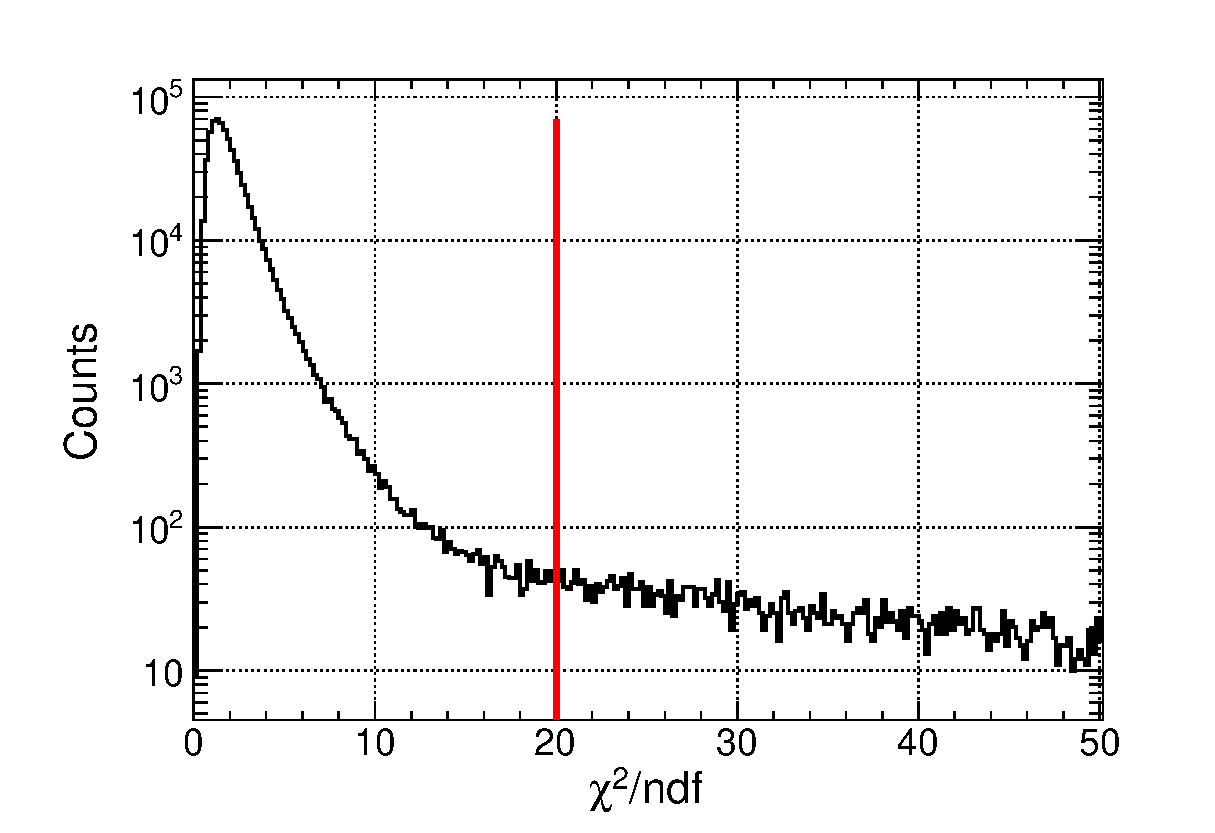
\includegraphics[width=12cm]{./fig/d5chi2.eps}
\caption[$\chi^2/ndf$ distribution in the fitting to connect BLC1 and BLC2 track. ]{$\chi^2/ndf$ distribution in the fitting to connect BLC1 and BLC2 track. $\chi^2/ndf<$20 was accepted.}
\label{fig-d5chi2}
\end{center}
\end{figure}  


\subsubsection{Comparison with the forward spectrometer\label{sec-beammom}}
To evaluate the absolute beam momentum, we used proton beam data to the PC. The proton beam momentum just upstream of T0 was analyzed with a TOF method between T0 and the PC, and was used as the reference. The details of an analysis method of a forward charged particle is described in Appendix B. Note that the momentum scale of the forward charged spectrometer was essentially determined by the detector geometry.

Figure \ref{fig-beamthrough} shows the comparison of the reconstructed momentum of the proton beam by the two spectrometers, beam line spectrometers (D5) and the forward charged particle spectrometer (PC), where a systematic difference between the two methods was observed. If it was due to the mis-alignment of the forward spectrometer, we need to modify the position of the PC by 10 cm order. It is more natural to suspect the beam spectrometer, which had many uncertainty in the magnetic field of the D5 and the relative positions of the drift chambers. Therefore, a linear correction function shown in Fig. \ref{fig-beamthrough}(left) was applied for the momentum reconstructed with the beam line spectrometer. Figure \ref{fig-beamthrough}(right) shows the distribution of the difference of the reconstructed momenta with the two methods after the correction. The distribution can be interpreted as a squared sum of the momentum resolution of the two methods. 

The momentum resolution of the T0-PC system was evaluated with a simulation to be 3.4 $\pm$ 0.3 MeV/$c$ for a proton beam with a momentum of 1 GeV/$c$. The simulation included the effects of multiple scatterings, energy losses and other physics processes. Realistic resolutions for drift chambers in Table \ref{tab-chmperformance} were also considered. The error was evaluated from the uncertainty in the intrinsic timing resolution of T0 and the PC. They were measured only with cosmic rays, namely minimum ionizing particles (MIPs), while a 1 GeV/$c$ proton deposits 1.5 times more energy and thus resulting in a better timing resolution. Here we assumed 0 and 25\% improvement of the timing resolution at maximum for 1 GeV/$c$ protons compared to MIPs. The average and the deviation of the resulting two momentum resolutions were employed as the resolution of the system and its error, respectively.

From the distribution in Fig. \ref{fig-beamthrough}(right) and the evaluated momentum resolution of the T0-PC system, the momentum resolution of the beam spectrometer was obtained to be 2.0 $\pm$ 0.5 MeV/$c$. The precision of the absolute momentum scale should be at the same level of that of the T0-PC system, which was evaluated to be $\sim$2 MeV/$c$ in Appendix B. The absolute scale will be further discussed as the missing mass scale in Sec. \ref{sec-scale}.

Figure \ref{fig-d5mom2} shows the kaon beam momentum distribution. % after the correction described above.
\begin{figure}[]
\begin{center}
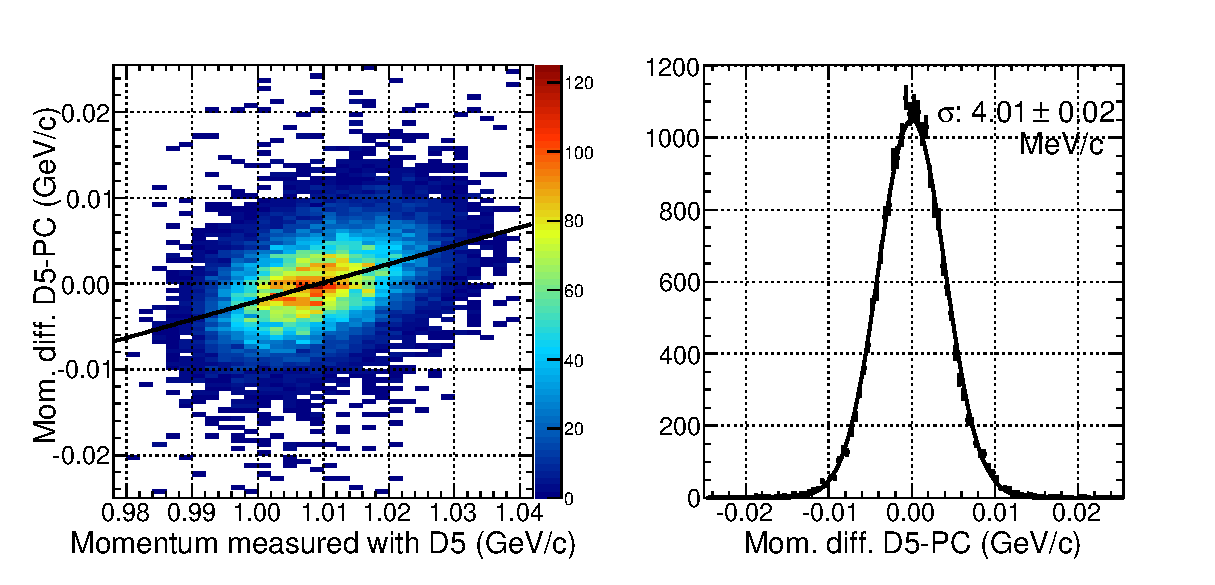
\includegraphics[width=\columnwidth]{./fig/pc-beamthrough.eps}
\caption[Comparison of the two reconstructed momenta with the beam-line spectrometer and the forward TOF spectrometer. ]{(left) Momentum dependence of the difference of reconstructed momenta with two different spectrometer, the beam-line spectrometer(D5) and the forward charged spectrometer(PC). (right) Distribution of the momentum difference after the correction with a linear function drawn in (left) with a black solid line.}
\label{fig-beamthrough}
\end{center}
\end{figure}  

\begin{figure}[]
\begin{center}
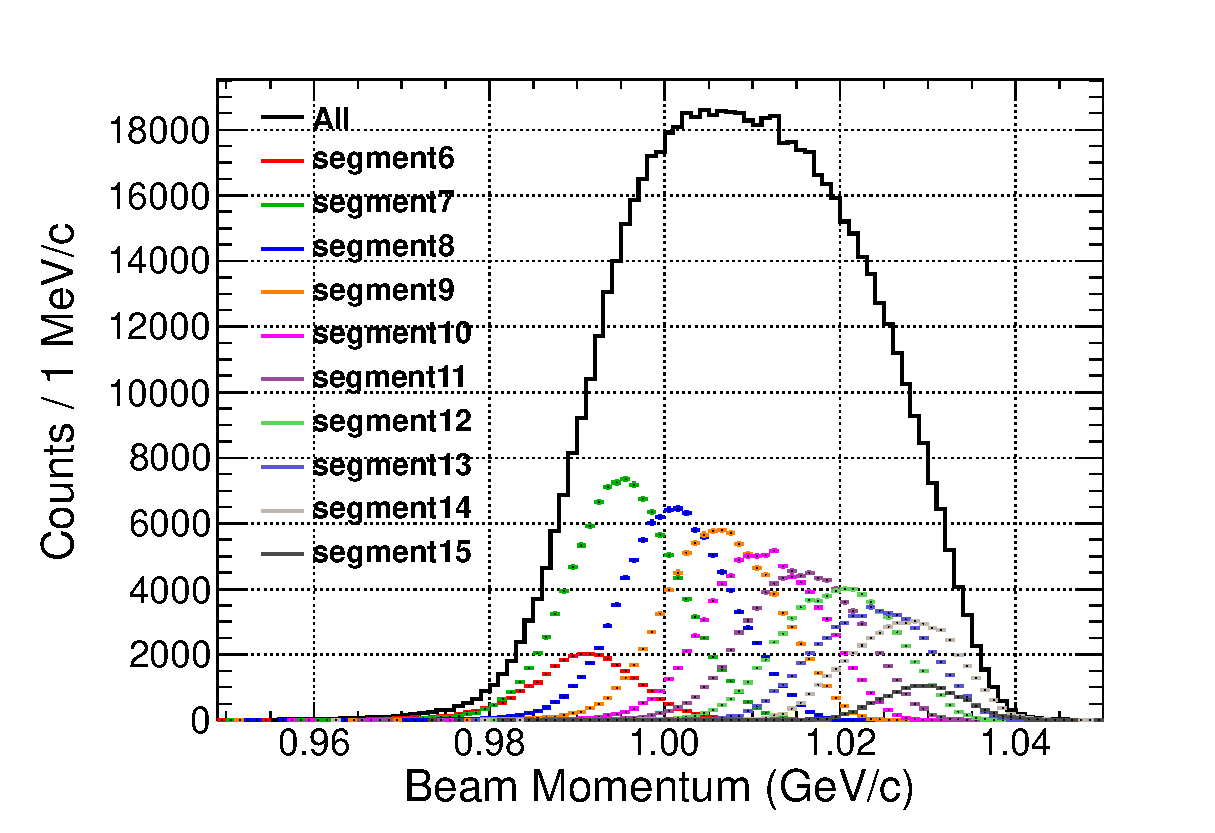
\includegraphics[width=12cm]{./fig/d5mom2.eps}
\caption[Distribution of the reconstructed beam momentum. ]{Distribution of the reconstructed beam momentum. Colored histograms represents the momentum distribution at each BHD segment.}
\label{fig-d5mom2}
\end{center}
\end{figure}  

\subsection{Event selection}
\subsubsection{Correlation between momentum and BHD hit}
Since the BHD position is located on a dispersive point, there is a clear correlation between the reconstructed kaon momentum and a hit segment of the BHD, which can be interpreted as the $x$ position at the BHD as shown in Fig. \ref{fig-bhdmom}. Fake combinations between a BHD hit and a BLC1-BLC2 track, mainly caused by kaon decays and pile-up particles, were rejected by applying three sigma cut on the distributions.

\begin{figure}[]
\begin{center}
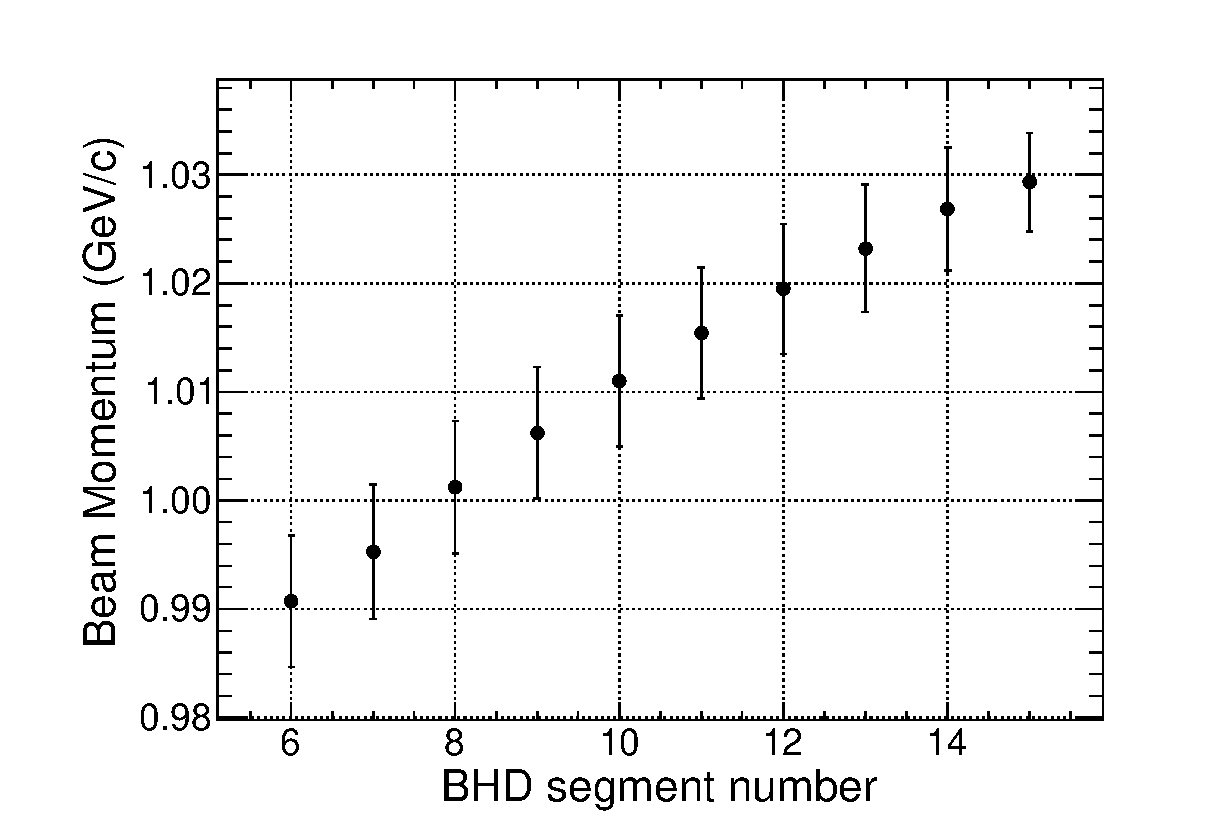
\includegraphics[width=12cm]{./fig/bhdmom.eps}
\caption[The relation between the hit segment of the BHD and the momentum distribution.]{The relation between the hit segment of the BHD and the momentum distribution. The mean value and the error bar represent the mean and sigma obtained by the Gaussian fitting of each colored distribution in Fig. \ref{fig-d5mom2}, respectively.}
\label{fig-bhdmom}
\end{center}
\end{figure}  

\subsubsection{Track matching between BLC2 and the BPC}
A portion of kaons also decay or react after identified by the AC. To reduce such events and to ensure the BPC track is the kaon beam, the track matching between BLC2 and the BPC was examined. Figure \ref{fig-blc2bpc} shows position and direction matchings, where three sigma cuts were applied for the BLC2-BPC track selection.

\begin{figure}[]
\begin{center}
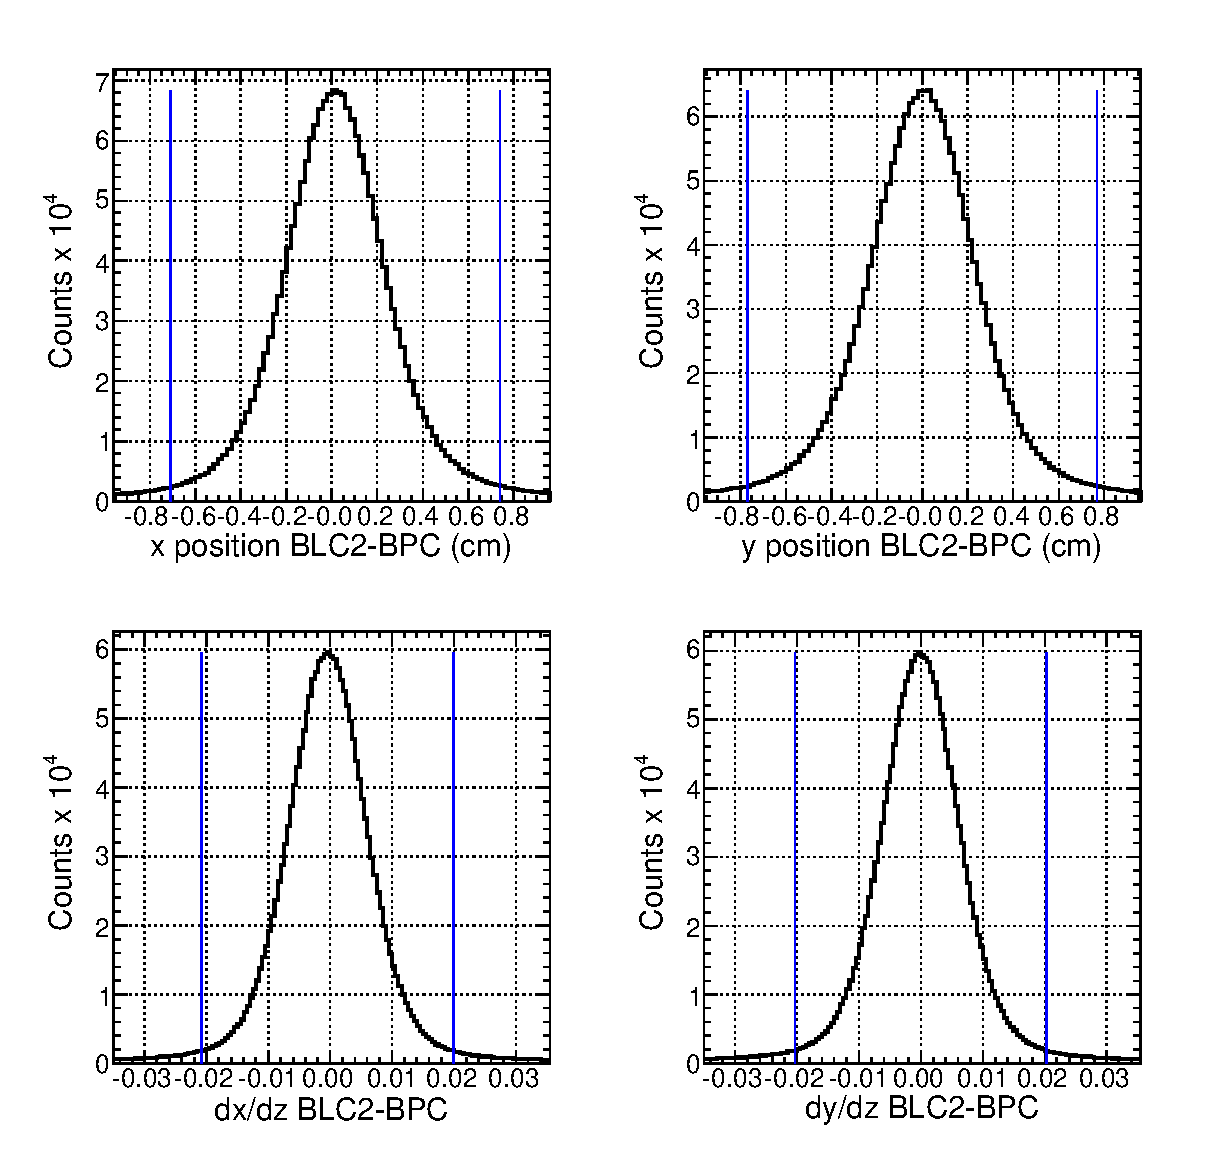
\includegraphics[width=14cm]{./fig/blc2bpc.eps}
\caption[Track matching between BLC2 and the BPC.]{Track matching between BLC2 and the BPC at $z=-75$ cm. The two blue vertical lines in each histogram define the accepted region.}
\label{fig-blc2bpc}
\end{center}
\end{figure}  

\subsubsection{Beam profile at the final focus point}
Figure \ref{fig-ffprof}(a) shows the kaon beam distribution at the final focus point evaluated by extrapolations of the BPC tracks. The target cell shape was clearly seen in Fig. \ref{fig-ffprof}(b), where the CDH trigger was requested. Although the beam spot size was a bit larger than the target size and the target cell was displaced from the center of the CDS, the position of the beam was well controlled on the target center. Note that the fiducial volume was defined in three-dimensionally as described in Sec.~\ref{sec-fiducial}.

\begin{figure}[]
\begin{center}
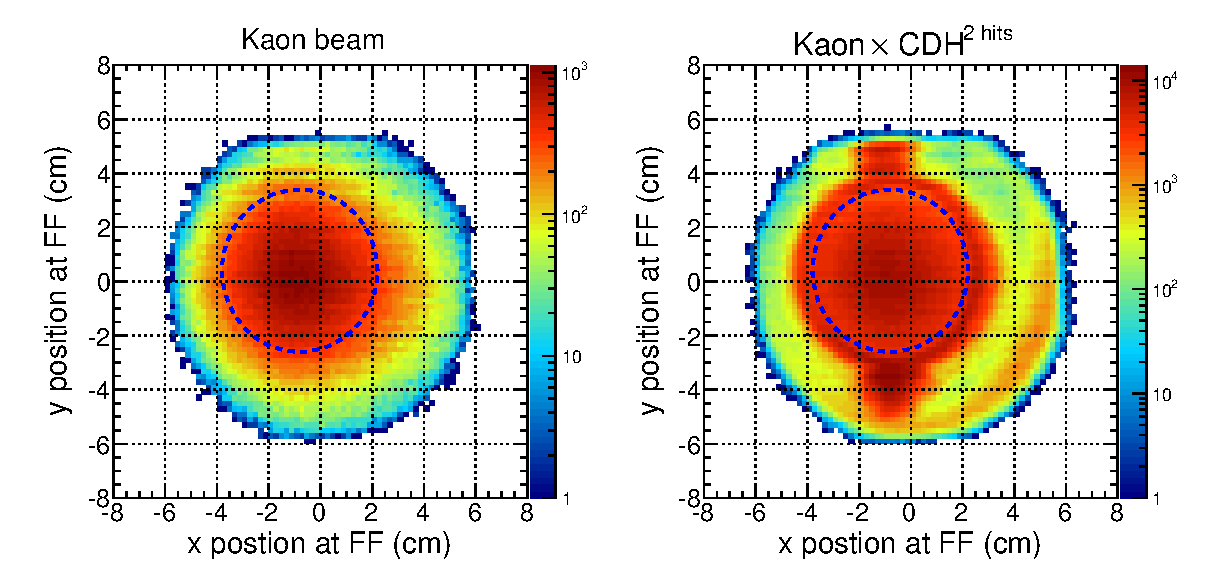
\includegraphics[width=\columnwidth]{./fig/ffprof.eps}
\caption[Kaon beam profile at the FF.]{Kaon beam profile at the FF (left) without any bias and (right) CDH 2 hits was required at a trigger level. The dotted circles represent the $xy$ fiducial region at the FF.}
\label{fig-ffprof}
\end{center}
\end{figure}  

\subsection{Luminosity evaluation\label{sec-luminosity}}
\subsubsection{Decay and reaction loss}
With the event selections described above, the kaon was guaranteed to be alive at the final plane of the BPC. Although the DEF hit was required at the trigger level, charged particles from kaon decays or reactions often hit on the DEF.

Therefore, we evaluated the decay and reaction loss probabilities between the plane 8 in the BPC ($z=-$18 cm) and the FF ($z$=0). For a fixed beam momentum of 1 GeV/$c$, kaon decay loss was calculated to be 2.4$\%$ with $c\tau$=3.712 m. The relative position uncertainty of $\sim$ 1 cm between the BPC and the FF gives 0.2\% systematic error. The effect of the $\sim$2\% beam momentum bite is smaller than 0.1\%. 
For the estimation of the reaction loss, the elementally $K^-N$ reaction cross section was simply scaled by the size of nucleus $A^{2/3}$. The materials considered in the evaluation were the DEF, the cap of the target vessel, the radiation shield and the target cell window. The total thickness was $\sim$0.67 g/cm$^2$ as summarized in Table \ref{tab-matbeam}. The reaction loss rate was obtained to be 0.7\% and the uncertainty of the estimation for the $K^-N$ reaction cross section was considered to give 20\% systematical error.

\subsubsection{Number of the target particle}
We defined the fiducial volume length as 10 cm, which is actually defined in three-dimensionally as shown in Fig. \ref{fig-cdcvertex}. The path length of the kaons in the fiducial volume was evaluated from the extrapolation of the BPC tracks using the unbiased kaon beam data. The normalized path length was obtained to be 10.03$\pm$0.02 cm. The error is evaluated by the time fluctuation during the production run.

The density of the helium-3 target was evaluated to be 0.0810$\pm$0.0002 as described in Sec. \ref{sec-target}.

\subsubsection{Kaon flux and integrated luminosity}
Finally, total kaon beam flux and the integrated luminosity used in the analysis was evaluated based on a scaler count of the kaon beam trigger, the analysis efficiency in the event selection, and the various factors discussed above. The event selection criteria and corresponding efficiencies are summarized in Table \ref{tab-beamflux}. 
The total kaon beam number incident on the target was evaluated to be ($3.31\pm0.06) \times 10^9$ and the integrated luminosity was to be 540$\pm$10 $\mu$b$^{-1}$. The errors associated to the kaon beam selection should be basically cancelled in calculating cross sections since the same event selections were applied in the data analysis and the integrated luminosity evaluation. However, time fluctuations of those survival rates, given as relative uncertainties in Table \ref{tab-beamflux}, were considered not to be cancelled.%, which was xx\% of the number of hardware kaon triggers.

\begin{table}[]
\caption[Typical values of the survival rate at each step of beam selection. ]{Typical values of the survival rate at each step of beam selection. Relative uncertainties of the survival rates in the kaon beam selection were determined by the fluctuations during the experimental period.}
\begin{center}
\begin{tabular}{l|ccc} 
\hline\hline					
		&	number		&	survival rate	&	relative uncertainty (\%)	\\
\hline									
Scaler number		&	7.52	$\times 10^9$	&	1	&		\\
\hline									
T0 single hit		&			&	0.950	&	0.3	\\
TOF kaon		&			&	0.973	&	0.2	\\
BPC single track		&			&	0.916	&	0.4	\\
BLC1\&2 single track		&			&	0.868	&	1.2	\\
BLC2-BPC connection		&			&	0.890	&	0.4	\\
momentum reconstruction		&			&	0.991	&	0.1	\\
									
\hline									
Fiducial selection at FF		&			&	0.696	&	1.0	\\
decay loss		&			&	0.976	&	0.2	\\
reaction loss		&			&	0.993	&	0.3	\\
\hline									
Total		&	3.31	$\times 10^9$	&	0.441	&	1.7	\\
\hline\hline									
Density	(g/cm$^3$)	&	0.081		&		&	0.3	\\
Thickness	(cm)	&	10.03		&		&	0.2	\\
\hline\hline												
Luminosity	($\mu$b$^{-1}$)	&	540		&		&	1.9	\\
\hline\hline												
\end{tabular}
\end{center}
\label{tab-beamflux}
\end{table}%

\section{Analysis of the cylindrical detector system\label{sec-anacds}}
The cylindrical detector system (CDS) is mainly used for the reconstruction of reaction vertex to derive the missing mass spectrum of the $^3$He$(K^-,n)$ reaction. However, more detailed analysis, such as particle identification and momentum reconstruction, was carried out to check the performance of whole spectrometer system. %In this section, the analysis and calibration method of the CDS presented. %Later in Sec, \ref{} the whole system performance will be checked in combination with the forward TOF counters.

An analysis procedure of the CDS is as follows:
\begin{enumerate}
\item Track finding in the CDC.
\item Search for associated hits on the IH and the CDH for each CDC track.
\item Reconstruct a vertex point with a beam track, and calculate mass-square of the CDC tracks.
\item Re-fit the CDC tracks after applying fine corrections on the CDC hits, and re-calculate the mass-square.
\item Identify particle species of each CDC track with a momentum and a re-calculated mass-square.
\item Re-calculate the vertex point, and obtain the momentum three-vector of each CDC track at the vertex.
\end{enumerate}

\subsection{Tracking with the CDC} 
A trajectory of a charged particle in a magnetic field can be expressed with a helix if the field is uniform. 
To check whether the helix can describe a charged track in the CDS,  a simulation data was generated in the calculated solenoid field by the TOSCA code. The simulation data was analyzed assuming the uniform field, and we confirmed that the helix can describe the charged particle tracks with a momentum precision better than 0.2\%. Therefore, the helix expression was employed for a CDC track.  
\subsubsection{Helix parametrization}
A helix at the CDC local coordinate can be parametrized as,%\cite{helix},
\begin{eqnarray*}
x(\phi) &=&d_\rho\cos\phi_0+\frac{1}{\rho}\left(\cos\phi_0-\cos(\phi_0+\phi)\right)\\
y(\phi) &=&d_\rho\sin\phi_0+\frac{1}{\rho}\left(\sin\phi_0-\sin(\phi_0+\phi)\right)\\
z(\phi) &=&d_z-\frac{1}{\rho}\tan\lambda\cdot\phi,
\end{eqnarray*}
where $d_\rho$ is the distance of the helix from pivotal point in the $xy$ plane, $\phi_0$ is the azimuthal angle to specify the pivotal point with respect to the helix center, $\rho$ is the inverse of the signed radius of the helix, $d_z$ is the distance of the helix from the pivotal point in the $z$ direction, and $\tan\lambda$ is the dip angle. The deflection angle $\phi$ is measured from the pivotal point, and specifies the position of the charged particle on the helical track. %The meanings of these parameters are depicted in Fig. \ref{fig-helix}.

The momentum of a charged particle is related to its helix parameters as,
\begin{eqnarray*}
{ \mathbf p} &=& \frac{cB}{\rho} \left( 
	\begin{array}{c}
	-\sin(\phi_0+\phi) \\	
	\cos(\phi_0+\phi) \\
	\tan\lambda
	\end{array}
	\right),
\end{eqnarray*}
where $c$ is the light velocity and $B$ is the strength of the magnetic field in the $z$ direction.

%\begin{figure}[]
%\begin{center}
%\includegraphics[width=\columnwidth]{./illustrator/helix.eps}
%\caption{}
%\label{fig-helix}
%\end{center}
%\end{figure}  

\subsubsection{TDC data conversion to the drift length}
A method to convert from a TDC channel to a drift time is the same as that for the beam line drift chambers described in Sec. 3.3.2. Relative time offset in each wire was adjusted in a similar way to the beam line chambers at first. For the conversion from a drift time to a drift length, a fifth order polynomial function was employed. The conversion function was iteratively adjusted by minimizing systematic shifts in the residuals as a function of the drift time. The residual was defined as subtracting the drift length from the shortest distance between the hit wire and the helix. A typical conversion function is shown in Fig. \ref{fig-cdcdtdl}. Note that additional fine tuning of the drift time was performed as described in Sec. 3.4.5.

\begin{figure}[]
\begin{center}
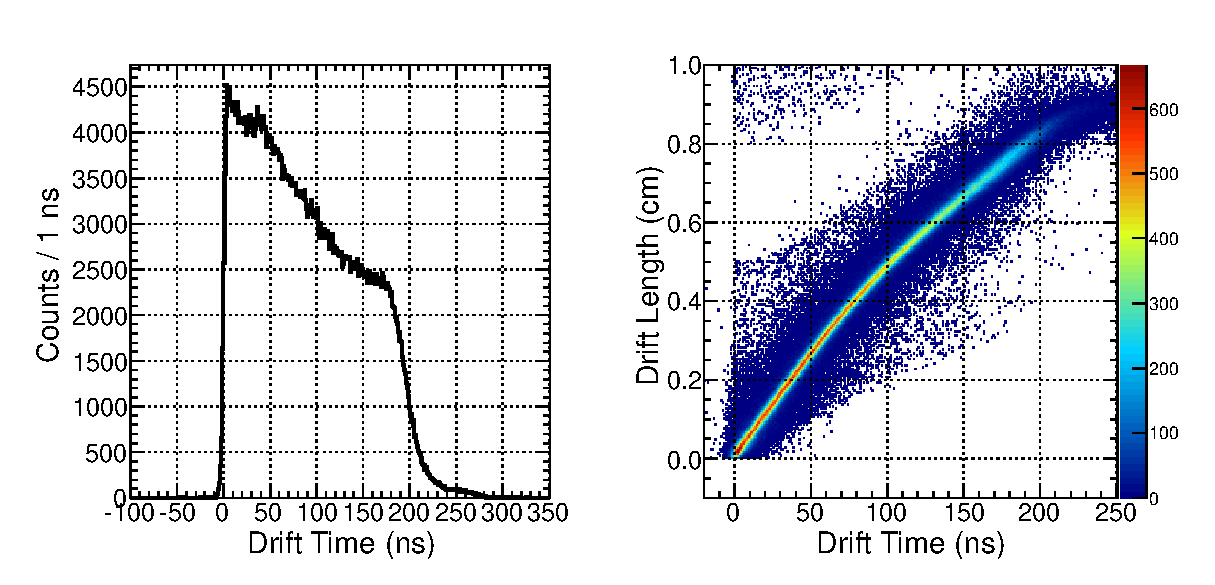
\includegraphics[width=\columnwidth]{./fig/cdcdtdl.eps}
\caption[Typical timing distribution and correlation between the drift time and the drift length of the CDC]{(left) Typical timing distribution of the CDC hit. (right) Typical correlation between the drift time and the drift length. }
\label{fig-cdcdtdl}
\end{center}
\end{figure}  

\subsubsection{Track finding and $\chi^2$ fitting}
First, track candidates were searched in $xy$ plane using only axial layers. A circle fitting was performed to determine the combination of hits in axial layers and to estimate helix parameters $d_\rho, \phi_0$, and $\rho$. %\cite{}. 
Then, associated hits in the stereo layers were searched in $z-\phi$ plane to estimate $d_z$ and $\tan\lambda$. Finally, full helix fitting was performed by using TMinuit to minimize the reduced-$\chi^2$, which was defined as,
\begin{eqnarray*}
\chi^2/ndf &=& \frac{1}{n-5}\sum_i^n \left(\frac{\delta_i-dl_i}{\sigma_i}\right)^2,
\end{eqnarray*}
where $n$ is the number of hits, $\delta_i$ is the shortest distance between the hit wire and the helix track, $dl_i$ is the drift length, and $\sigma_i$ is the spatial resolution of 180 $\mu m$ obtained in Sec. \ref{sec-cdcposres}. The resultant $\chi^2/ndf$ distribution is shown in Fig. \ref{fig-cdcchi} and tracks with $\chi^2/ndf < 30$ were defined as good tracks. Note that bad $\chi^2/ndf$ tracks were used in the multiplicity counting in the CDS.

A track was required to have at least one hit in each axial super layer. In addition, at least 5 hits in the stereo layers and at least 10 hits in total were required.
\begin{figure}[]
\begin{center}
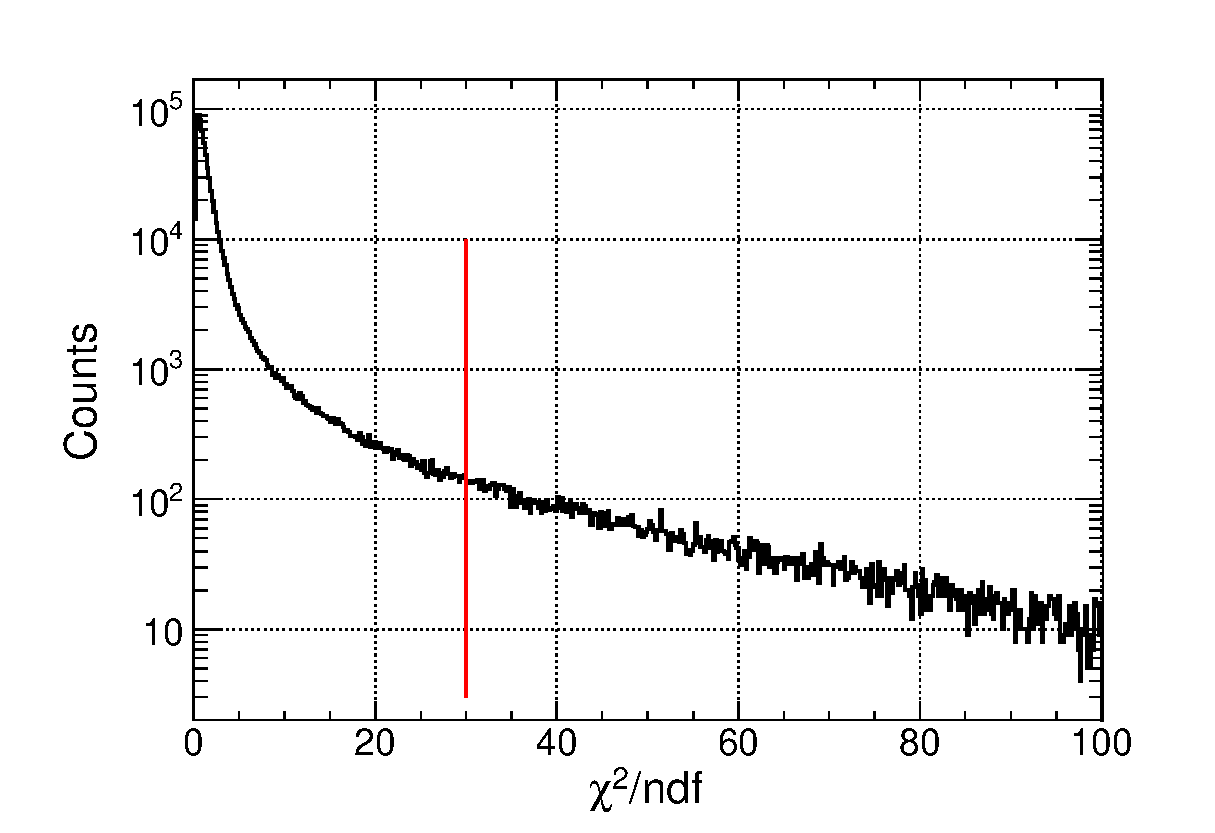
\includegraphics[width=12cm]{./fig/cdcchi.eps}
\caption[$\chi^2/ndf$ distribution in the CDC tracking. ]{$\chi^2/ndf$ distribution in the CDC tracking. Tracks with $\chi^2/ndf<$ 30 were accepted.}
\label{fig-cdcchi}
\end{center}
\end{figure}  

\subsection{Associated hit search in the IH and the CDH}
Once a CDC track was defined, associated hits in the IH and the CDH were determined by using extrapolated position of the track. Figure \ref{fig-cdchodo}(left) shows the azimuthal angle matching for the CDH at the inner radius of r = 544 mm when we obtained only one track in the CDC and one hit in the CDH. The matching efficiency is obtained to be better than 99\%.
In a general case, we also checked the matching at the outer radius of the CDH, r = 574 mm and accepted CDC tracks with multiple CDH hits. If multiple hits in the CDH was associated with one CDC track, the fastest timing segment was defined as the timing of the CDC track. 
For the IH, similar procedure was applied. Figure \ref{fig-cdchodo}(right) shows the azimuthal angle matching of the IH at the inner radius of r = 137 mm. The matching efficiency was $\sim$ 98\%.

\begin{figure}[]
\begin{center}
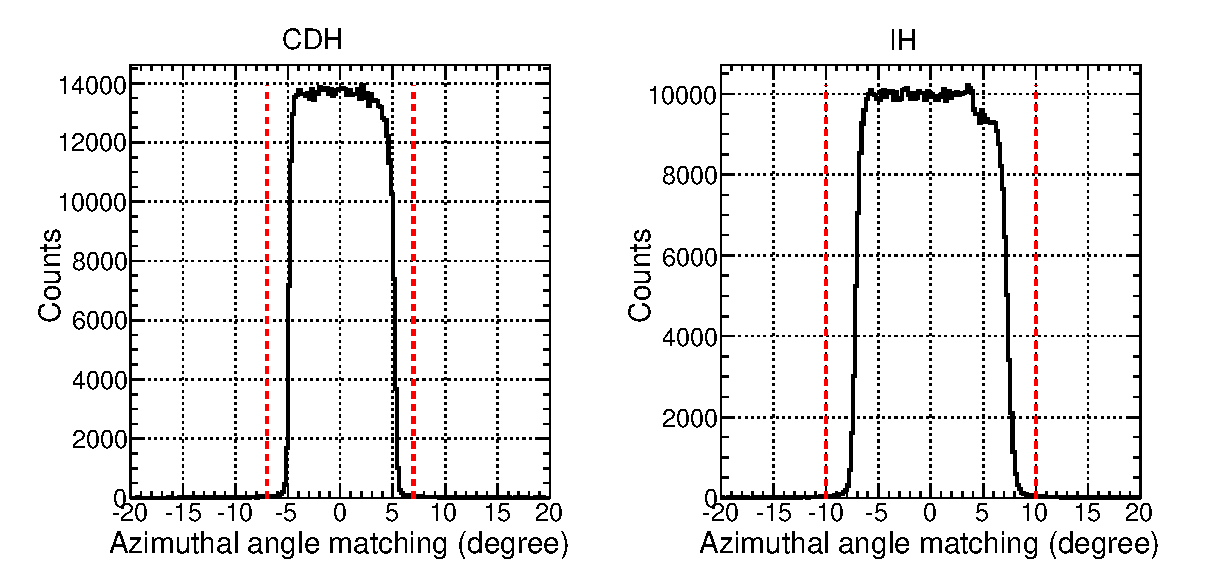
\includegraphics[width=\columnwidth]{./fig/cdc-ihcdhmatch.eps}
\caption[Azimuthal matching between a CDC track and a CDH/IH hit.]{Azimuthal matching of hits (left) on the CDH and (right) on the IH. Events between two red lines were accepted. The segment size corresponds to $\pm5^\circ$ and $\pm7.5^\circ$ for the CDH and the IH, respectively. }
\label{fig-cdchodo}
\end{center}
\end{figure}  

\subsection{Vertex reconstruction}
\subsubsection{Vertex with one CDC track}
With one CDC track, a candidate of the reaction-vertex point was obtained by the distance of the closest approach (DCA) using the BPC and the CDC track. The point on the BPC was defined as the candidate of the vertex as shown in Fig. \ref{fig-vertexreconstruction}(left). %Figure \ref{} is a schematic explanation.

\subsubsection{Vertex with two CDC tracks}
If an event had two or more CDC tracks, all possible pairs among them were examined to reconstruct a secondary vertex. The secondary vertex was defined as the center of DCA points of the two helical tracks. The momenta of the two tracks were recalculated at the secondary vertex with an energy loss correction, and the parent track was reconstructed. Then, the primary vertex, i.e. the reaction vertex, was obtained using the BPC track and the parent track and the DCA was used to selection of the vertex candidates as shown in Fig. \ref{fig-vertexreconstruction}(right).% as schematically shown in Fig. \ref{}.
\\

Among the vertex candidates obtained with one and two CDC tracks, the minimum DCA candidate was selected to be the reaction vertex. Figure \ref{fig-cdcdca}(left) shows the track multiplicity of the CDC with a neutron detection by the NC, and the Fig. \ref{fig-cdcdca} shows the difference of the DCA distribution due to the number of CDC tracks used to reconstruct the reaction vertex. In Fig. \ref{fig-cdcdca}(right), $\pi^+\pi^-$ pairs were analyzed and the difference of the vertex reconstruction method was found to be not so significant. Note that the displacement of the $z$-vertex position by 1 cm causes only $\sim$0.3 MeV/$c$ momentum deviation for a 1 GeV/$c$ neutron, which is much smaller than the precision of the current experiment. 


\begin{figure}[]
\begin{center}
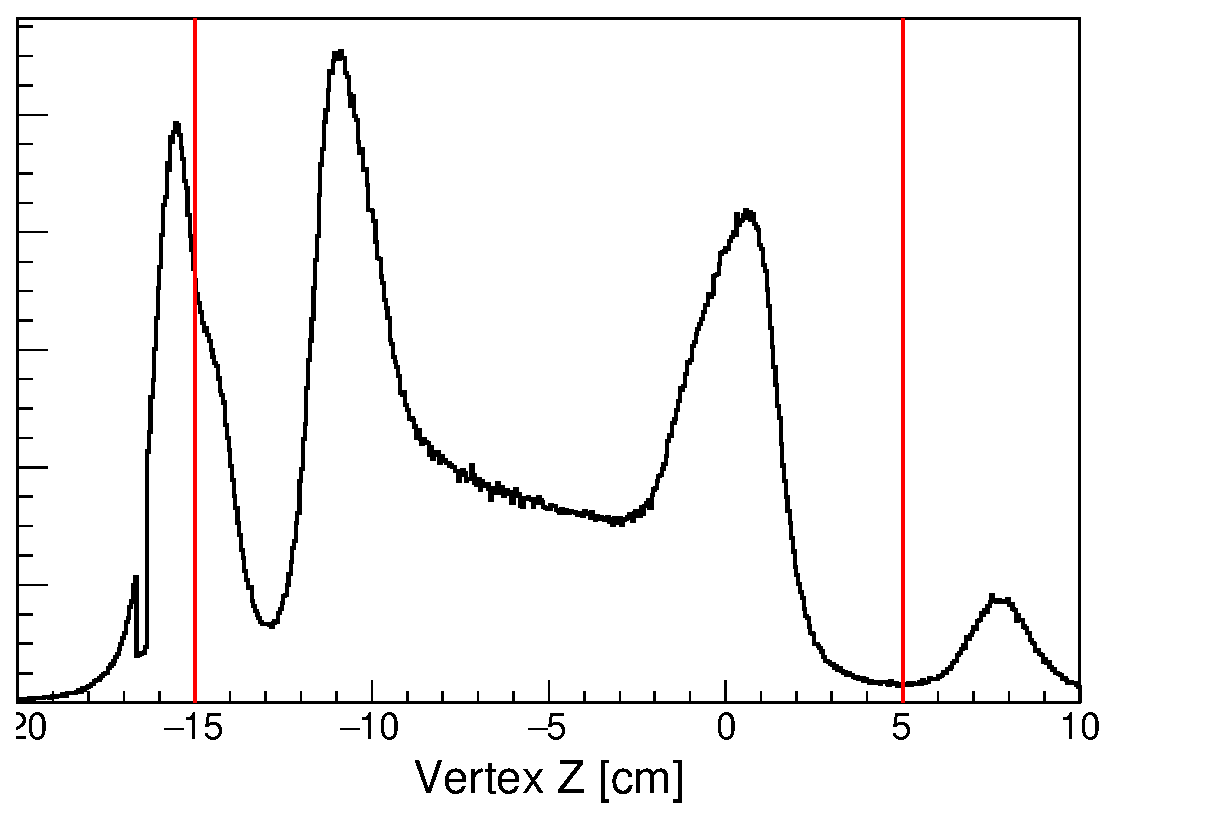
\includegraphics[width=\columnwidth]{./illustrator/vertex.eps}
\caption[Vertex reconstruction with BPC and CDC tracks.]{Vertex reconstruction with BPC and CDC tracks.}
\label{fig-vertexreconstruction}
\end{center}
\end{figure}  
\begin{figure}[]
\begin{center}
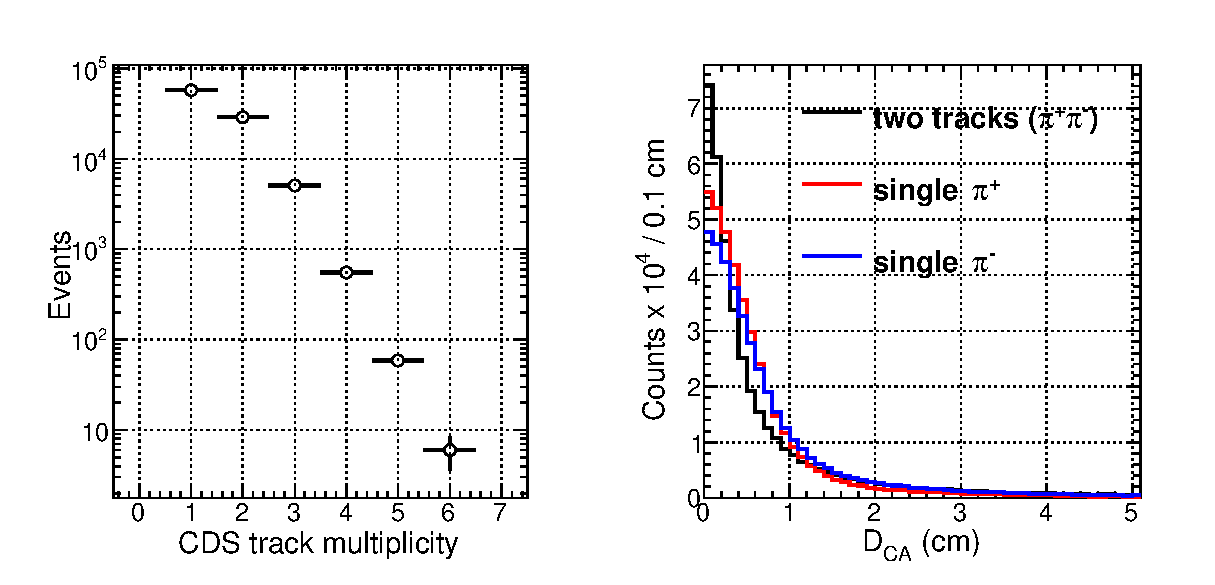
\includegraphics[width=\columnwidth]{./fig/cdc-mul.eps}
\caption[CDC track multiplicity and DCA distributions.]{(left) CDC track multiplicity. Neutron detection by the NC is requested. (right) DCA distributions of the events with $\pi^+\pi^-$ pairs detected by the CDS. The black, red, and blue histograms are obtained by using reconstructed parent track of the $\pi^+\pi^-$, the $\pi^-$ track, and the $\pi^+$ track, respectively.}
\label{fig-cdcdca}
\end{center}
\end{figure}  

\subsection{Particle identification}\label{sec-cdcpid}
A velocity $\beta$ and a mass $M$ of the CDC track can be calculated as,
\begin{eqnarray}
\beta &=& \frac{L_{CDC_{in}-CDH}}{\left((T_{CDH}-T_{T0}) - T^{calc}_{T0-vertex}- T^{calc}_{vertex-CDC_{in}} \right)\times c} \label{eq-cdsbeta}\\
%&&T^{calc}_{T0-vertex} = \frac{L_{T0-vertex}}{ \beta_{beam}c}\\
M^2&=&p^2\times \frac{1-\beta^2}{\beta^2},
\end{eqnarray}
where $\it{L_{CDC_{in}-CDH}}$ is the helical-track length between the entrance of CDC tracking volume at the radius of 15.1 cm and the CDH, $T_{CDH}$ - $T_{T0}$ is the measured flight time between the CDH and T0. $T^{calc}_{T0-vertex}$ and  $T^{calc}_{vertex-CDC_{in}}$ are calculated flight times between T0 and the vertex, and between the entrance of the CDC tracking volume and the CDH, respectively. Velocity and curvature changes by energy losses were taken into account. % as the detail is explained in Appendix \ref{}. 

The resultant distribution of the momentum versus the mass-square is shown in Fig. \ref{fig-cdspid2d}, where pions, kaons, protons and deuterons are clearly separated. In the current analysis, a particle identification is roughly done by using only the mass-square and the charge as shown in Fig. \ref{fig-cdspid1d}. Although the PID efficiencies are high at around 99\%, we did not remove electrons, positions and muons contaminated in the pion identification. Those contamination can be much suppressed if we used two dimensional particle identification in the mass-square and the momentum plane. 

\subsubsection{CDH calibration}
The velocity of the particle can be also calculated using the measured momentum ($p$) and the particle mass ($m_x$) as,
\begin{eqnarray}
\beta_{calc}=\sqrt{\frac{m_x^2+p^2}{p^2}}. \label{eq-cdsbeta2}
\end{eqnarray}
Timing offsets and time-walk effects were adjusted so that the difference of measured $\beta$ in Eq. \ref{eq-cdsbeta} and calculated $\beta_{calc}$ in Eq. \ref{eq-cdsbeta2} became zero by using pions.
% and then we required the mass-squared to be within $\pm 3\sigma$ of its momentum dependent resolution represented as,
%\begin{eqnarray*}
%\sigma_{M_2}^2 &=& 4M^4\left(\frac{\sigma_p(p)}{p}\right)^2+4p^2c^2(p^2+M^2)\left(\frac{\sigma_{TOF}}{L_{CDC_{in}-CDH}} %\right)^2,
%\end{eqnarray*}
%where $\sigma_p(p)$ is a momentum resolution evaluated in Sec \ref{} and $\sigma_{TOF}$ is the resolution of the time of flight measurement. Atypical timing resolution of 160 ps is used for $\sigma_{TOF}$ here. Since $L_{CDC_{in}-CDH}$ is different track by track, we can not draw exact boundaries of particles in Fig. \ref{fig-cdspid}.% Instead, we shows the distribution of accepted events in Fig. \ref{}.
\begin{figure}[]
\begin{center}
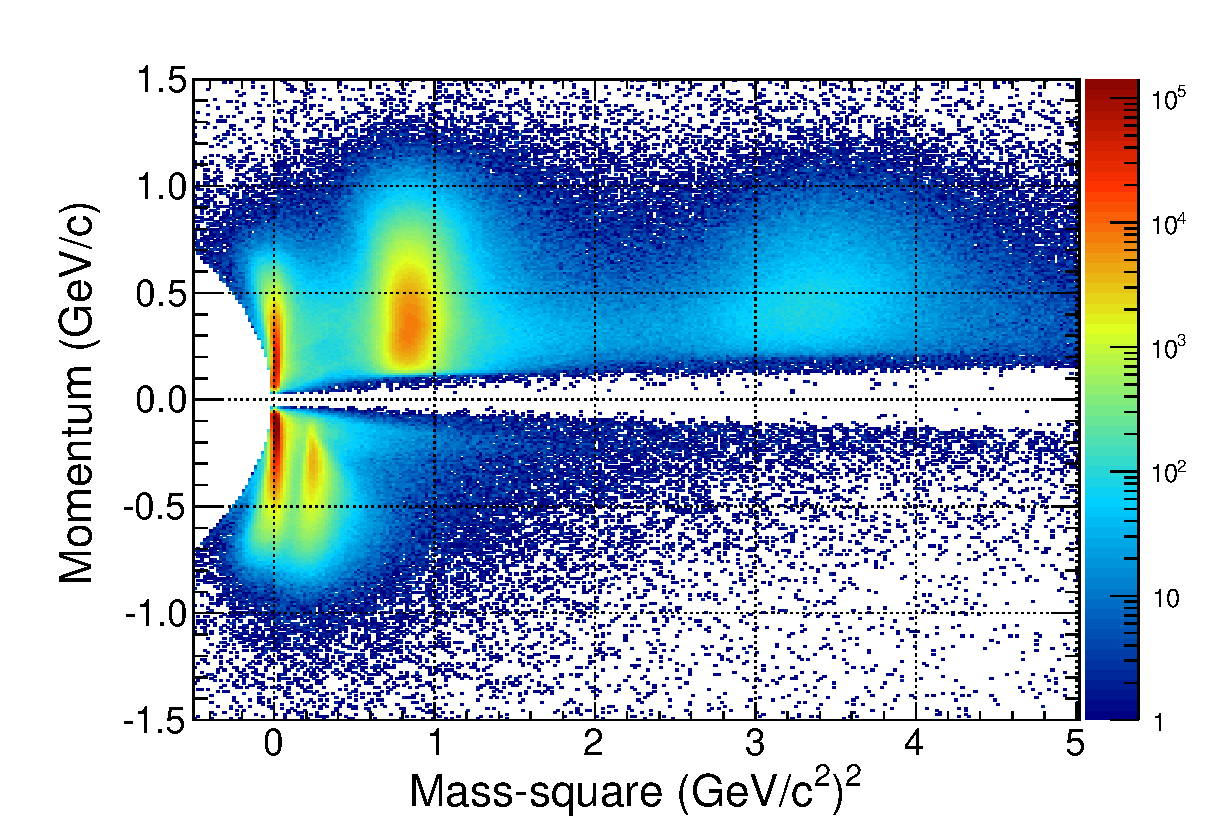
\includegraphics[width=12cm]{./fig/cdcpid2d.eps}
\caption[Two-dimentional PID plot for the CDS particle]{PID plot for the CDS particle. $\pi^+$, protons and deuterons are clearly separated in the positive momentum side, while $\pi^-$ and $K^-$ are in the negative side.}
\label{fig-cdspid2d}
\end{center}
\end{figure}  

\begin{figure}[]
\begin{center}
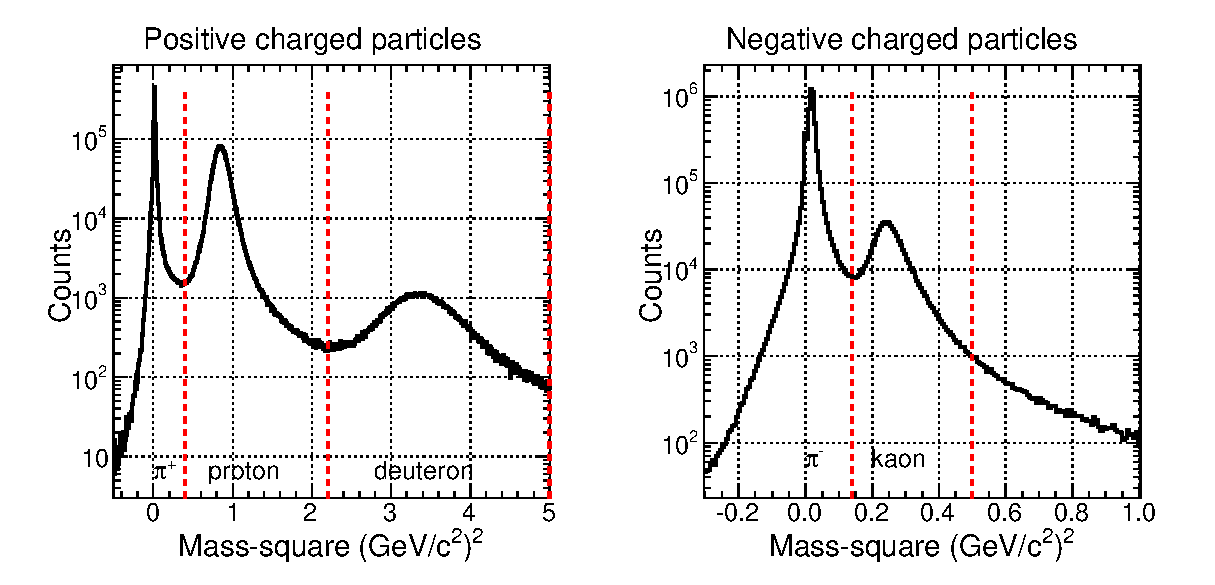
\includegraphics[width=\columnwidth]{./fig/cdcpid1d.eps}
\caption[Mass-square distributions of the CDS particles.]{Mass-square distributions for (left) positive and (right) negative charged particles in the CDS. Particle identification is roughly done with red dotted lines. }
\label{fig-cdspid1d}
\end{center}
\end{figure}  

\subsection{Fine corrections}\label{sec-cdsfinetune}
Following two corrections on the CDC drift time were applied to minimize systematic effects caused by different particle species and the momenta.
\subsubsection{Re-timing of the CDC drift times}
Since the TDC start timing was defined by the T0 timing, the TDC data of the CDC contained the drift time and flight time between T0 and the CDC cell. To extract the drift time, we calculated the flight time by using the helical trajectory, the associated CDH-hit timing, and the velocity calculated in Eq. \ref{eq-cdsbeta}.
\subsubsection{Time-walk effect on the CDC drift times}
A time-walk effect is well known for photon sensors and collected by using the correlation of the integral charge or the pulse height. % as explain in Sec. \ref{}. 
A similar effect should exist in a drift chamber. Although we took only timing information, a pulse height of a CDC signal should be correlated with an evaluated velocity $\beta_{CDC}$. Figure \ref{fig-cdcslew} shows clear correlation between the $1/\beta^2_{CDC}$ and the residual converted to a time scale. This correlation was compensated by fitting with a function $p_0 + p_1x +p_2x^2+ p_3\exp(p_4x)$ as shown in Fig. \ref{fig-cdcslew}. 
\begin{figure}[]
\begin{center}
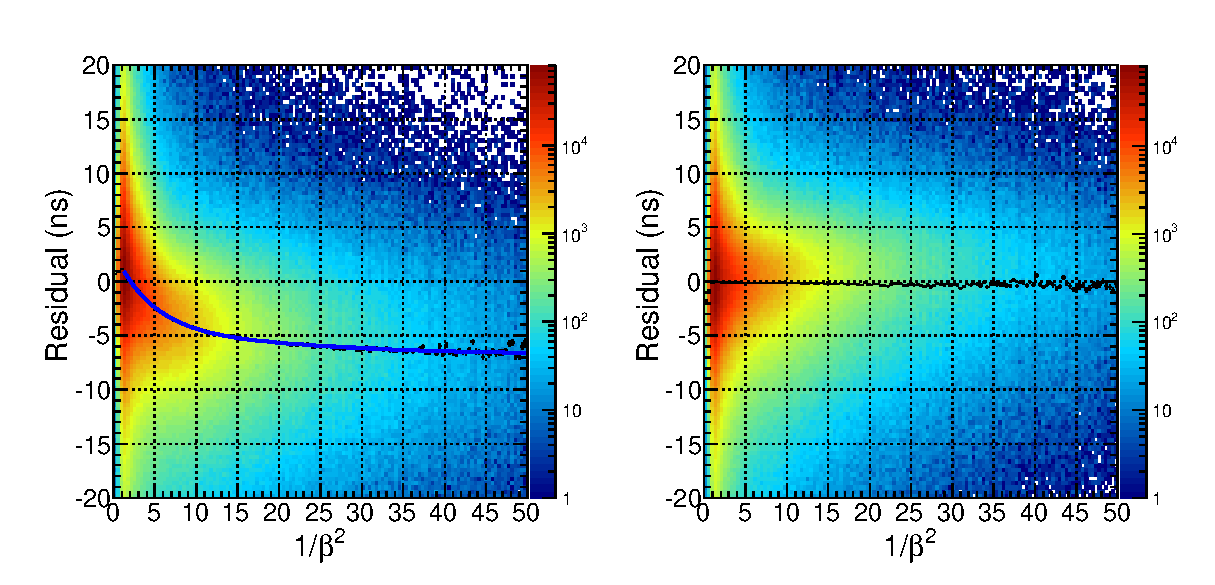
\includegraphics[width=\columnwidth]{./fig/cdcslew.eps}
\caption[Correlation between the 1/$\beta^2$ and the residual of the CDC track]{Correlation between the 1/$\beta^2$ and the residual of the CDC track, (left) before and (right) after fine corrections.}
\label{fig-cdcslew}
\end{center}
\end{figure}  


\subsection{CDS performance}
\subsubsection{Spatial resolution of planes\label{sec-cdcposres}}
Figure \ref{fig-cdcresid} shows the typical residuals. The residuals are compared with those obtained by a Monte-Carlo simulation assuming various spatial resolutions. From the comparison, the spatial resolution in the experimental data was evaluated to be $\sim$180 $\mu$m. This value was used in the Monte-Carlo simulation in this thesis.

As for the systematic differences by the particle species, typical residual distributions are compared in Fig. \ref{fig-cdcresidpikp}. No significant differences were observed.
\begin{figure}[]
\begin{center}
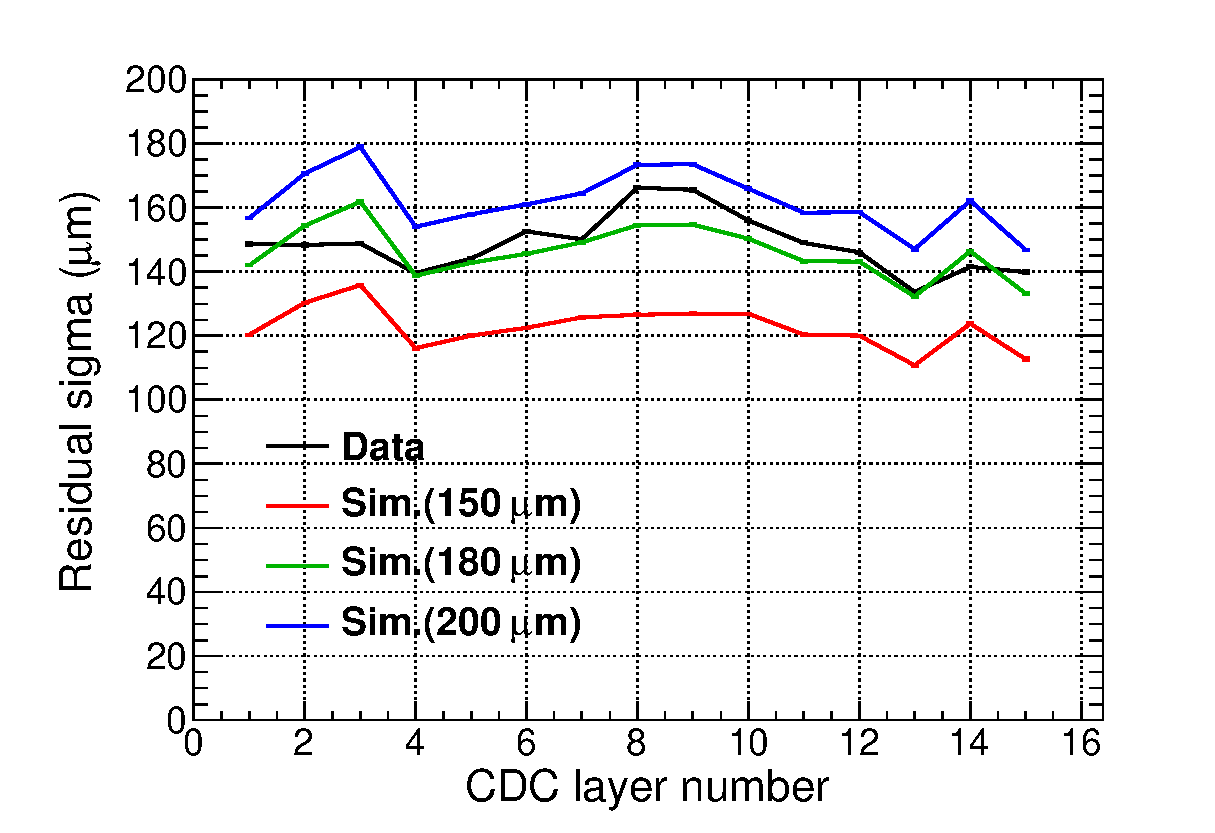
\includegraphics[width=12cm]{./fig/cdcresid.eps}
\caption[Residual distributions of the CDC.]{Comparison of the residual distributions of the CDC between the data and the simulation. The simulation with an intrinsic spatial resolution of 180 $\mu$m agrees with the data.}
\label{fig-cdcresid}
\end{center}
\end{figure}  

\begin{figure}[]
\begin{center}
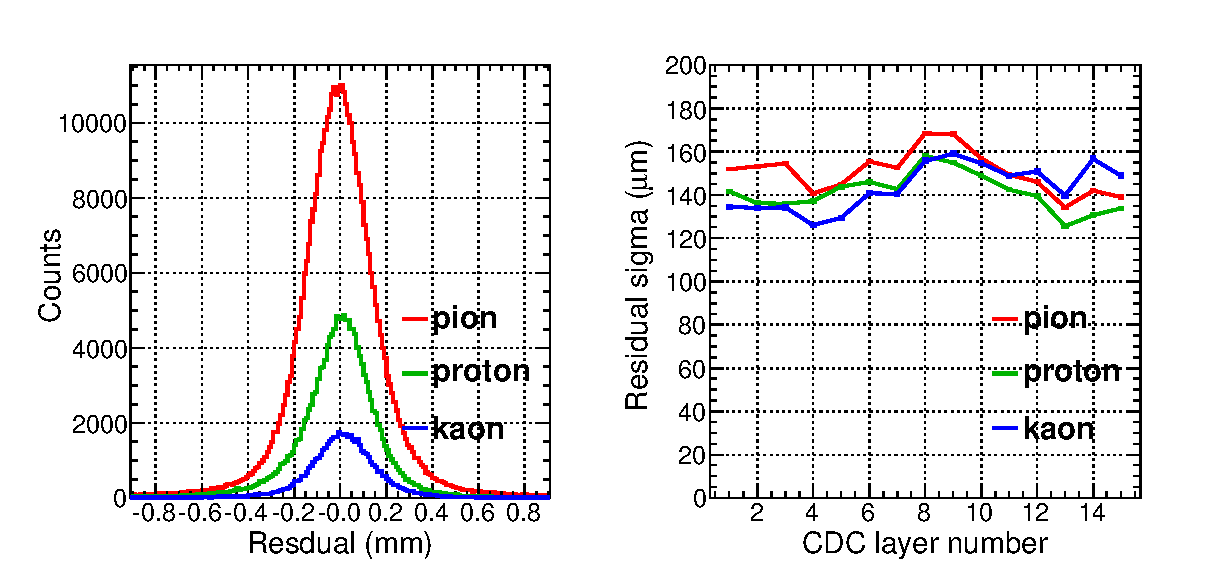
\includegraphics[width=\columnwidth]{./fig/cdcresidpikp.eps}
\caption[Particle dependences of the CDC performances.]{Particle dependences of (left) the shape of the residual distributions and (right) the residuals as a function of the layer number.}
\label{fig-cdcresidpikp}
\end{center}
\end{figure}  

\subsubsection{Momentum resolution}
A transverse momentum resolution for the CDC track was evaluated by the Monte Calro simulation with the spatial resolution as derived above. Figure \ref{fig-cdcsimres} shows the resolutions for pions, kaons and protons.
\if0 Their momentum dependences are expressed as,
\begin{eqnarray*}
\left(\frac{\delta p_t}{p_t}\right) &=& a \cdot p_t + \frac{b}{p_t-c}+d \\
\end{eqnarray*}
where a, b, c, and d are parameters. The obtained parameters are summarized in Table \ref{tab-pikpres} for each particle species. %These were used for particle identification as described in Sec. \ref{sec-cdcpid}.
\fi
\begin{figure}[]
\begin{center}
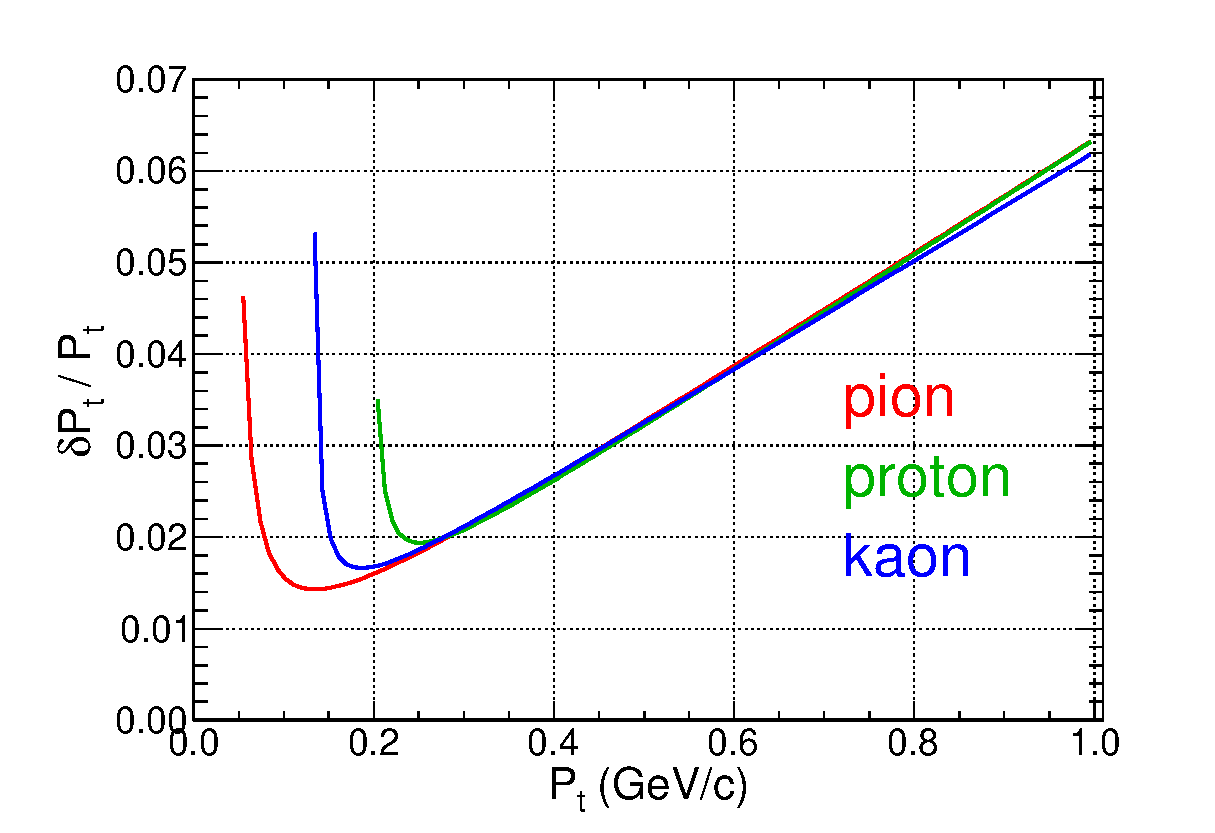
\includegraphics[width=12cm]{./fig/cdcsimres.eps}
\caption{The simulated $p_t$ resolution of the CDC single track for each particle species.}% The points are simulated data and the solid curves are the fit.}
\label{fig-cdcsimres}
\end{center}
\end{figure}  

\if0
\begin{table}[]
\caption{Parameters of the $p_T$ resolutions for each particle species.}
\begin{center}
\begin{tabular}{l|cccc} 
\hline\hline				
particle	&	a		&	b		&	c		&	d		\\
\hline													
$\pi$	&	6.29	$\times 10^{-2}$	&	5.38	$\times 10^{-4}$	&	4.22	$\times 10^{-2}$	&	1.04	$\times 10^{-5}$	\\
kaon	&	5.97	$\times 10^{-2}$	&	1.87	$\times 10^{-4}$	&	1.30	$\times 10^{-1}$	&	2.17	$\times 10^{-3}$	\\
proton	&	6.32	$\times 10^{-2}$	&	2.00	$\times 10^{-4}$	&	1.95	$\times 10^{-1}$	&	-5.62	$\times 10^{-5}$	\\
\hline\hline												
\end{tabular}
\end{center}
\label{tab-pikpres}
\end{table}%
\fi

\subsubsection{CDC tracking efficiency \label{sec-cdceff}}
Tracking efficiencies of CDC were evaluated by using two data samples; one was the cosmic-ray data obtained in the off-spill duration, and the other was the physics data, i.e., secondary charged particles from kaon-induced reactions.

For the cosmic-ray data, we selected events with two separated hits on both the IH and the CDH, which should contains two CDC tracks generated by one cosmic-ray. These event samples are expected to be clean enough since they are almost free from accidentals and neutral particles. For the cosmic data, we obtained the tracking efficiency of 97.8 $\pm$ 0.2\%. The error was evaluated from the fluctuations during the experimental period. 

In contrast, the kaon-induced data is expected to contain much more backgrounds. To reduce the background contributions from beam-pileup events and neutral particles, strict cuts were applied as follows:
\begin{enumerate}
\item The beam was required to be a single particle and hit on the target.
\item Select single-CDH-hit events with more than 5 MeV$ee$ (electron equivalent) energy deposits on both CDH PMTs. Timing selection was applied to exclude $\gamma$-ray events.
\item The azimuthal-angle difference between the CDH and the IH hit-segments was required to be less than 20$^\circ$.
\end{enumerate}
With this event selection, the tracking efficiency was obtained to be 94.0 $\pm$ 0.5\%. The error was evaluated in the same way as the cosmic-ray data.

Although there is some discrepancy in the obtained efficiencies, the two data-samples would give extreme cases of the measurement conditions. Therefore, we adopted the mean values of 96 $\pm$ 2\% in the current analysis, where the error was evaluated from the deviation.
%The stability of the CDC tracking efficiency is plotted in Fig. \ref{}.
\subsubsection{Vertex resolution\label{sec-cdsvres}}

The vertex resolution was evaluated with the kaon-induced tracks. The vertex was reconstructed for every CDC track with the beam track. As for the resolution in the $xy$ plane, the reconstructed vertices around $x(y)$=0, $z$=0 cm were selected and the $y(x)$ position distribution was checked.  In Fig. \ref{fig-cdcposres}(left) two clear peaks which correspond to the target cell with 0.3 mm thickness are observed. As a result of Gaussian fitting of these peaks, the $xy$ vertex resolution was evaluated to be $\sim$1 mm, which was almost solely determined by the resolution of the beam track.
Figure \ref{fig-cdcposres}(right) shows $z$ vertex distribution with $x^2+y^2<2$ cm$^2$. The largest peak around $-$16 cm corresponds to the DEF. By fitting the DEF peak and considering the DEF thickness of 3 mm, the $z$ vertex resolution was evaluated to be $\sim$7 mm. Both $xy$ and $z$ vertex resolutions are consistent with those obtained by the simulation.
\begin{figure}[]
\begin{center}
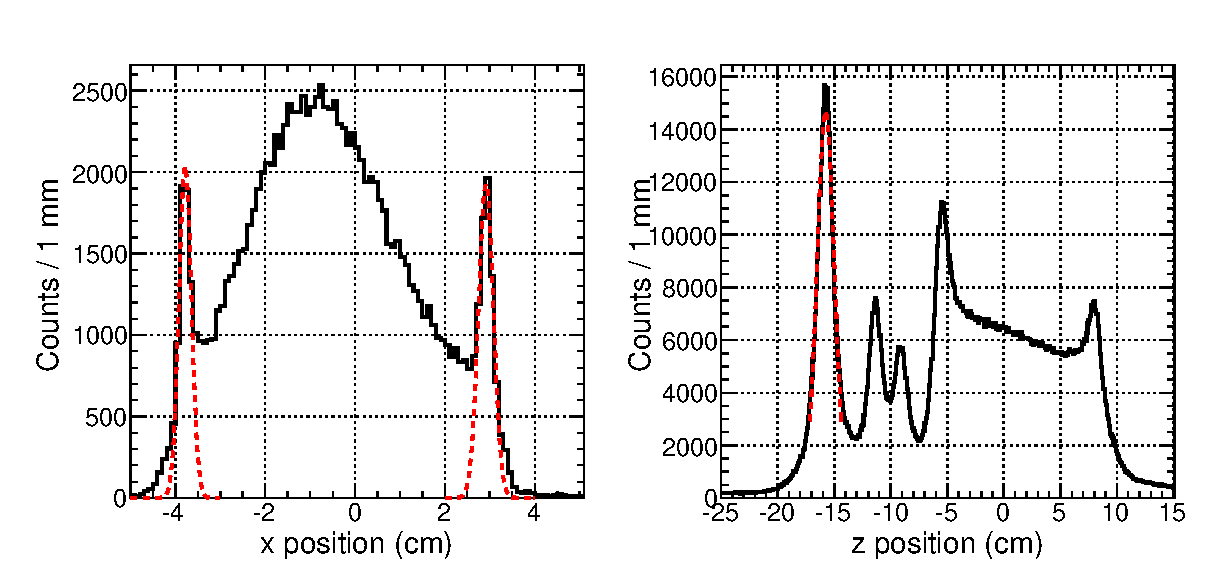
\includegraphics[width=\columnwidth]{./fig/cdcxyres.eps}
\caption[$x$ and $z$ vertex position distributions.]{(left) Reconstructed $x$ vertex position distribution around $y$=$z$=0 cm. The two distinct peaks correspond to the target cell. (right) Reconstructed $z$ vertex position distribution. The most prominent peak at around $z=-$16 cm is the position of the DEF. The red dotted lines are the Gaussian fitting results to evaluate the vertex resolutions.}
\label{fig-cdcposres}
\end{center}
\end{figure}  

\subsection{Fiducial volume selection\label{sec-fiducial}}
The vertex distribution in the $zy$ plane and the $zx$ plane are shown in Fig. \ref{fig-cdcvertex}. The target cell is clearly identified in addition to the DEF, the vacuum vessel, the thermal radiation shield, and the $^3$He transfer pipes. The fiducial volume of the $^3$He target is defined as the blue boxes in Fig. \ref{fig-cdcvertex}, whose size is 30 mm radius $\times$ 100 mm length. The fiducial volume is apart from the beryllium cylinder of the target cell by more than 3 times the $xy$ resolution to reduce contaminations from other materials. The $z$ length and position of the fiducial volume is defined by that of the beryllium cylinder to avoid material complexity in other parts of the cell.  
\begin{figure}[]
\begin{center}
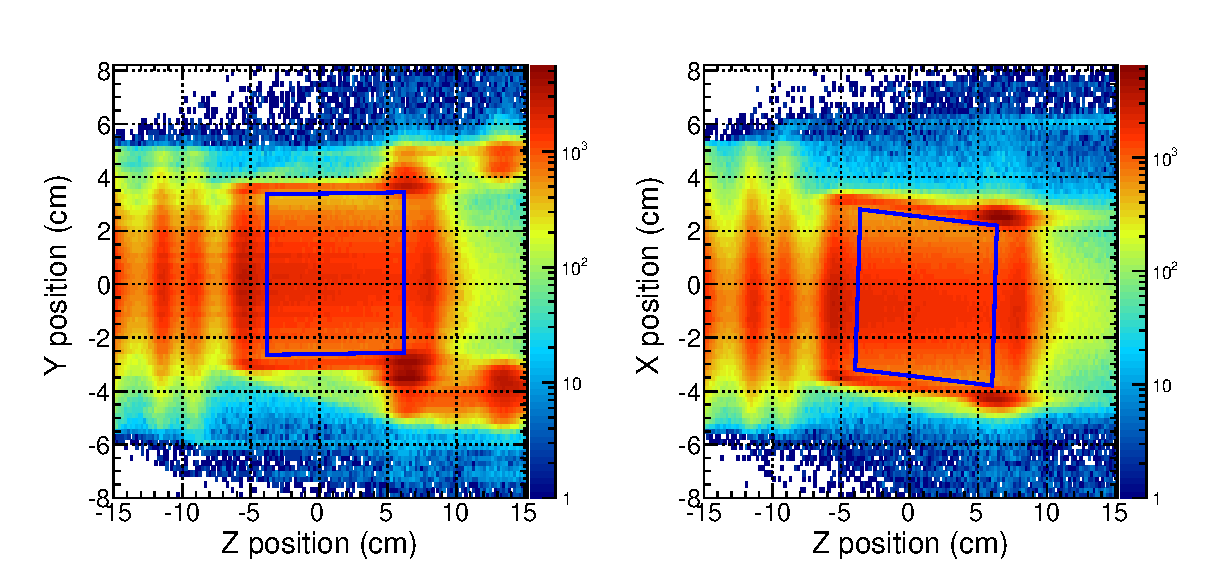
\includegraphics[width=\columnwidth]{./fig/cdcvertex.eps}
\caption[Definition of the fiducial volume.]{Reconstructed vertex distribution in (left) the $zy$ and (right) the $zx$ planes. The fiducial volume is defined as the blue boxes. }
\label{fig-cdcvertex}
\end{center}
\end{figure}  

\subsection{$K^0_s$ and $\Lambda$ reconstruction\label{sec-cdck0}}
To confirm the spectrometer performance of the CDS,  the invariant masses of $\pi^+\pi^-$ pairs and $p\pi^-$ pairs were reconstructed as shown in Fig. \ref{fig-cdck0}  and Fig. \ref{fig-cdclambda}, respectively. Clear peaks of $K^0_s\to\pi^+\pi^-$ and $\Lambda\to\pi^-p$ decays were obtained in the invariant mass distributions. Their positions are consistent with PDG values within 1 MeV/$c^2$ precision after an adjustment of the field strength of the solenoid magnet described below. %The peak widths are also consistent with those obtained by the simulation.
\begin{figure}[]
\begin{center}
\includegraphics[width=10cm]{./fig/cdck0.eps}
\caption[Invariant mass distribution of $\pi^+\pi^-$ pairs reconstructed with the CDS. ]{Invariant mass distribution of $\pi^+\pi^-$ pairs reconstructed with the CDS. The $K^0_s$ peak was fitted with a Gaussian and a third-order polynomial background. The red solid curve and the blue dotted curve show the fitting result and background contribution, respectively.}% The vertical dotted lines show the $K^0_s$ selection region in the later analysis. }
\label{fig-cdck0}
\end{center}
\end{figure}  

\begin{figure}[]
\begin{center}
\includegraphics[width=10cm]{./fig/cdclambda.eps}
\caption[Invariant mass distribution of $p\pi^-$ pairs reconstructed with the CDS. ]{Invariant mass distribution of $p\pi^-$ pairs reconstructed with the CDS. The $\Lambda$ peak was fitted with a Gaussian and a third-order polynomial background. The red solid curve and the blue dotted curve show the fitting result and background contribution, respectively.}% The vertical dotted lines show the $\Lambda$ selection region in the later analysis.}
\label{fig-cdclambda}
\end{center}
\end{figure}  

\subsubsection{Adjustment of the CDS field strength}
Since we were not able to measure the magnetic field strength of the CDS in the final setup, the value should be adjusted by using the data. $K^0_s$ and $\Lambda$ peaks are good calibration source for this purpose. The field strength was changed a little so that the both peak positions were consistent to the PDG values with in 1 MeV/$c^2$ as shown in Fig.~\ref{fig-cdcfield}. We found the requirement is satisfied when the magnetic field is 
\begin{eqnarray}
0.715   \pm 0.002\ {\rm T}, 
\end{eqnarray}
where the error was assumed to be symmetric.

\begin{figure}[]
\begin{center}
\includegraphics[width=10cm]{./fig/cdcfield.eps}
\caption[Optimization of the CDS field strength.]{The correlation between the peak position deviations of $K^0_s$ and $\Lambda$ from the PDG values and the CDS field. The center value of the CDS field is set to be 0.715T.  }
\label{fig-cdcfield}
\end{center}
\end{figure} 

\if0 % appendix??
\subsection{Topological selection}
In the CDS analysis, we sometimes applied topological selection to improve the signal-to-noise ratio. 
\subsubsection{CDC single track analysis}
If we analyze single track of the CDC, there is only one parameter $D_{CA}$ (Fig. \ref{}) to define the property of the topology. The typical $D_{CA}$ distribution is shown in Fig. \ref{}.
\subsubsection{CDC two track analysis}
As shown in Fig. \ref{}, three parameters $D_{CA}^{CDC}$, $D_{CA}^{beam}$ and $D_{vertex}$ appear in two track analysis. Their typical distributions are show in Fig. \ref{} for $K^0_s$
\fi
\section{Analysis of forward neutrons \label{sec-ananc}}
\subsection{Analysis method}
A momentum of a forward neutral particle is measured by the time-of-flight method between T0 and the NC. % as schematically illustrated in Fig. \ref{fig-ncconcept}. 
The velocity of the forward particle can be expressed as,
\begin{eqnarray}
\beta_{nc} &=& \frac{L_{vertex-NC} }{(T^{measured}_{T0-NC}-T^{calc}_{T0-vertex})\times c} \label{eq-ncbeta}
\end{eqnarray}
where, $L_{vertex-NC}$ is the flight length between the hit position on the NC and the reaction vertex obtained by the BPC and the CDC as described in Sec. 3.4.3, $T^{measured}_{T0-NC}$ is the measured flight time between T0 and the NC, and $T^{calc}_{T0-vertex}$ is the calculated time between T0 and the vertex by using reconstructed beam momentum. The hit position on T0 was obtained from an extrapolation of the BLC2 track, and the momentum decrease of the kaon beam due to the energy losses in the spectrometer materials were considered.

%Note that the current analysis method always requires at least one CDC track and unavoidably make bias in the final spectrum.

\subsection{NC hit selection}
To obtain the flight time of the neutral particle and its hit position on the NC, we selected the time-wise first-hit segment of the NC whose energy deposit was above the offline analysis threshold. The hit positions in the $x$- and $z$-directions were defined as the center of the segment, and that in $y-$direction was evaluated from the time difference of the two PMT signals on both ends of the segment. To convert from the time difference to the $y$ position, we used the effective light propagation velocity of 14 cm/ns, which was measured with a $^{90}$Sr checking source.

\subsection{Charge removal}
There were two scintillation counter arrays, the BVC and the CVC, between the target and the NC. To assure neutral-particle detection with the NC, no signal in the BVC and the CVC was required. The time range of the TDCs for those counters were set to 200 ns, whose full range was used for the simplicity to veto forward-going charged particles. The over veto efficiency is evaluated in Sec. \ref{sec-overveto}.

\subsection{1/$\beta$ distribution}
Figure \ref{fig-ncbeta} shows $1/\beta$ distribution of the neutral particles without offline threshold of the energy deposit on the NC. Hardware-wise, we set the threshold of discriminators to around 0.5 MeV$ee$. The distribution shows a distinct $\gamma$-ray peak at $1/\beta=1$, with which we calibrated the relative time offset of the NC counters and the T0 counters. In the slower velocity region, namely the larger $1/\beta$ region, continuous distribution of neutrons can be seen. The TDCs used for the NC had 200 ns time ranges and we adjusted the start timing to detect the particles with ($-$25, 175) ns offset to the gamma-ray TOF. It corresponds to down to 200 MeV/$c$ neutrons. A peak structure around $1/\beta=1.3$ is the so-called quasi-free peak attributed to the reactions of $``p"(K^-,n)K^0_s$ and $``n"(K^-,n)K^-$. Our interested region is between the $\gamma$-ray peak and the quasi-free peak, where a clear gap is observed. This shows the low background condition in our measurement. The accidental background yield can be directly evaluated with the strength of the left part of the $\gamma$-ray peak.

\subsubsection{Particle identification}
The neutral particles with $1/\beta>1.1$ were identified as neutrons, whereas gate for $\gamma$-rays were defined to be (0.9,1.1). Then, we can obtain the neutron momentum $p_n$ with the neutron mass $m_n$,
\begin{eqnarray}
p_n &=& \frac{m_n}{\sqrt{\frac{1}{\beta^2}-1}}.
\end{eqnarray}

\begin{figure}[]
\begin{center}
\includegraphics[width=12cm]{./fig/nc-beta.eps}
\caption[1/$\beta$ distribution of the forward neutral particles.]{1/$\beta$ distribution of the forward neutral particles detected with the NC. Right hand side of the dotted vertical line is identified as neutrons, while the hatched area represents the $\gamma$ selection. }
\label{fig-ncbeta}
\end{center}
\end{figure}  
 
\begin{figure}[]
\begin{center}
\includegraphics[width=12cm]{./fig/nc-betade.eps}
\caption{Distribution of the energy deposit on the NC and 1/$\beta$.}
\label{fig-ncbetade}
\end{center}
\end{figure}  

Figure \ref{fig-ncsn}(left) shows the $1/\beta$ distribution sliced in the various energy deposit regions. As naturally expected, the background contribution decreases with the higher energy deposit region. To quantitatively discuss this tendency, purity of the signal, $S/(S+B)$, is plotted as a function of energy deposit region in Fig. \ref{fig-ncsn}(right). Here we integrated the events in $1/\beta$=(1.15,1.35) as $S+B$ and the contribution of the accidental background $B$ was evaluated by fitting the spectrum in $1/\beta$=(0.6,0.9) with a constant function. We set the offline threshold to 8 MeV$ee$ where the purity almost saturates.

\begin{figure}[]
\begin{center}
\includegraphics[width=\columnwidth]{./fig/nc-sn.eps}
\caption[Typical spectra with energy deposit slices and neutron purity dependence on the energy deposit.]{(left) Typical spectra with energy deposit slices. The horizontal lines shows the background level. Events in the hatched area were counted to derive the neutron purity. (right) Neutron purity dependence on the energy deposit. The offline analysis threshold was set to 8 MeV$ee$ as indicated with a red line.}
\label{fig-ncsn}
\end{center}
\end{figure}  


\subsection{Momentum resolution\label{sec-ncres}}
%\subsubsection{Threshold dependence}
%Another point is the resolution of neutron momentum. It is naturally expected that the resolution get better with a higher threshold. The resolution was evaluated by fitting $\gamma$-ray peak with a Gaussian. Figure \ref{} shows the threshold dependence of the $1/\beta$ resolution ($\sigma$) of the system.

\subsubsection{Momentum dependence}
The $1/\beta$ resolution of the neutral particle can be decomposed as,
\begin{eqnarray*}
\sigma_{\frac{1}{\beta}}\left(\frac{1}{\beta}\right) &=& \frac{1}{L_{vertex-NC}}\sqrt{\left(\frac{\sigma_z^{NC}}{\beta}\right)^2+\left(\left(\frac{1}{\beta}-\frac{1}{\beta_{beam}}\right)\cdot\sigma_z^{vertex}\right)^2+c^2\sigma_t^2}.
\end{eqnarray*}
The first term is a contribution from the uncertainty in the $z$ hit position of the NC. Assuming a uniform $z$ distribution of the hit position, $\sigma_z^{NC}=$5 cm/$\sqrt{12}$=1.44 cm is obtained. The second term is caused by the uncertainty of the $z$-vertex position. The $z$-vertex resolution was evaluated to be $\sigma_z^{vertex}$=0.7 cm in Sec. \ref{sec-cdsvres}. The last term comes from the intrinsic time resolution of T0 and the NC measured to be $\sim$110 ps with cosmic-ray data.

However, the measured $\gamma$-ray resolution cannot be reproduced by those values. Other effects such as the uncertainty in the $xy$ position, the neutral particles not from the reaction point, and the distortion of the flight length by scatterings might contribute. Here we made two independent assumptions to reproduce the resolution: additional deteriorations of $\sigma_t$ or $\sigma_z^{nC}$. The former has no $\beta$ dependence, namely the time measurement had worse resolution for some reasons, while the latter has the $\beta$ dependence which comes from the uncertainty in the flight length measurement. The data can be reproduced by deteriorating $\sigma_t$ from 110 ps to140 ps or $\sigma_z^{NC}\sim$ from 1.44 to 3 cm. The two cases were plotted in Fig. \ref{fig-ncresol} for the 1/$\beta$ and the neutron momentum resolutions. We adopted the mean of the two lines as the resolutions for the current analysis, and the deviation was considered as a systematic error. The neutron momentum resolution at $K^-pp$ binding threshold ($\sim$1.2 GeV/$c$) was evaluated to be 8.0$\pm$0.4 MeV/$c$.

\begin{figure}[]
\begin{center}
\includegraphics[width=\columnwidth]{./fig/nc-resol.eps}
\caption[Resolutions of the 1/beta and the neutron momentum.]{Resolutions of (left) the 1/beta and (right) the neutron momentum. The two curves correspond to the two independent assumptions in the resolution evaluation.}
\label{fig-ncresol}
\end{center}
\end{figure}  

\subsubsection{Stability and uniformity}
The $\gamma$-ray peak position and its resolution were stable during the experiment as shown in Fig. \ref{fig-ncrun}.  We also checked the uniformity of the 112 segments. % Figure \ref{} and Fig. \ref{} show the kaon-induced hit distributions of $\gamma$-rays and neutrons, respectively. The events has the continuous distributions.
Figure \ref{fig-ncseg} shows all the segment in the NC worked and calibrated fine.
\begin{figure}[]
\begin{center}
\includegraphics[width=\columnwidth]{./fig/nc-run.eps}
\caption[Run dependence of the $\gamma$-ray peak position and its resolution.]{Run dependence of (top) the $\gamma$-ray peak position and (bottom) its resolution.}
\label{fig-ncrun}
\end{center}
\end{figure}  
\begin{figure}[]
\begin{center}
\includegraphics[width=\columnwidth]{./fig/nc-seg.eps}
\caption[NC segment dependence of the $\gamma$-ray peak position and its resolution.]{NC segment dependence of (top) the $\gamma$-ray peak position and (bottom) its resolution. The hatched areas represent the difference of the NC layers.}
\label{fig-ncseg}
\end{center}
\end{figure}  

\section{Missing mass resolution\label{sec-mmresol}}
The missing mass resolution $\sigma_{M_X}$ of the $^3$He($K^-,n$) reaction is expressed as,
\begin{eqnarray}
\sigma_{M_X}=c\times\sqrt{\left(\frac{\partial M_X}{\partial p_{beam}}\right)^2(\sigma_p^{beam})^2+\left(\frac{\partial M_X}{\partial p_{neutron}}\right)^2(\sigma_p^{neutron})^2},
\end{eqnarray}
where $\sigma_p^{beam}$ and $\sigma_p^{neutron}$ are the momentum resolutions of the kaon beam and the forward-going neutron, respectively. The contribution of the reaction-angle resolution is not considered since it is negligibly small ($<$7 mrad). The momentum resolution of the kaon beam is 2.0 $\pm$ 0.5 MeV/$c$ as discussed in Sec. \ref{sec-beammom} and that of the neutron is discussed in Sec. \ref{sec-ncres}. The missing mass resolution at the reaction angle of 0 degree with the beam momentum of 1 GeV/$c$ is shown in Fig. \ref{fig-mmresol}. The resolution satisfied our experimental requirement of $\sim$10 MeV/$c^2$ resolution at the region of interest.

\begin{figure}[]
\begin{center}
\includegraphics[width=12cm]{./fig/mm-resol.eps}
\caption[Missing mass resolution of the $^3$He($K^-,n$) reaction.]{Missing mass resolution of the $^3$He($K^-,n$) reaction. The vertical dotted line and the hatched area represent the $K^-pp$ binding threshold and the region of interest, respectively.}
\label{fig-mmresol}
\end{center}
\end{figure}  

\section{Precision of the missing mass scale\label{sec-scale}}
To determine absolute missing mass scale of the $^3$He($K^-,n$) reaction, the beam momentum was calibrated at first by the forward-proton spectrometer as described in Sec. \ref{sec-beammom}. Then the neutron momentum was evaluated by reconstructing the invariant masses of $\Sigma^\pm\to n\pi^\pm$ decays. In addition, we checked the the residual-nucleus peaks in the missing masses of $^3$He($K^-,nK^0_s)d$, $^3$He($K^-,npK^-)p$, and $^3$He($K^-,np\pi^+\pi^-)n$ reactions. In these studies, the neutron and the charged particles were measured with the NC and the CDS, respectively.

\subsection{Reconstruction of the $\Sigma$s and the residual nucleus}
\subsubsection{$\Sigma$ reconstruction}
The $\Sigma^\pm$ hyperons are mainly produced by quasi-free processes of $K^-+p\to\pi^\mp\Sigma^\pm$. The forward-going $\Sigma$s were reconstructed by detecting $\Sigma^\pm \to \pi^\pm n$ decays, where the pion and the neutron were measured with the CDS and the NC, respectively. The reconstructed $\pi^\pm n$ invariant mass distributions are shown in Fig. \ref{fig-sigmaraw}, where $\Sigma^\pm$ peaks are clearly identified. Since two pions are emitted from the $K^-+p\to\pi^\mp\Sigma^\pm$ reactions, the signal-to-noise ratios of the $\Sigma^\pm$ would increase by requiring an additional pion. Red histograms in Fig. \ref{fig-sigmaraw} are the $n\pi^\pm$ invariant mass spectra with the two pion selection, and we evaluated the peak position of the $\Sigma^\pm$ using the histograms. Since the neutron momentum from $\Sigma$ decay has wide distribution with rather large statistics, the peak positions were evaluated for five $^3$He($K^-,n)X$ missing-mass ranges; (2.27,2.37), (2.37,2.47), (2.47,2.57), (2.57,2.67), and (2.67,2.77) GeV/$c^2$.

\begin{figure}[]
\begin{center}
\includegraphics[width=\columnwidth]{./fig/sigma-raw.eps}
\caption[Invariant mass distributions of $n\pi^+$ and $n\pi^-$.]{Invariant mass distributions of (left) $n\pi^+$ and (right) $n\pi^-$. The red histograms require $n\pi^+\pi^-$ detection and the $^3$He($K^-,n\pi\pi)X$ missing mass to be consistent with a deuteron. They are scaled by factor two.}
\label{fig-sigmaraw}
\end{center}
\end{figure}  

\subsubsection{Spectator deuteron in quasi-free $K^0_s$ production}
In the quasi-free reactions on a proton in the $^3$He target, the spectator is a deuteron or a pair of a neutron and a proton. Especially in the quasi-free $K^0_s$ production, $K^-+p\to K^0_s+n$, we can easily identify the spectator by using the $K^0_s\to \pi^+\pi^-$ decay and the forward-going neutron detected with the CDS and the NC, respectively. As shown in Fig. \ref{fig-k0missd}(left), clear strength around the deuteron mass can be seen in the $^3$He($K^-,nK^0_s)X$ missing mass. By requesting the small missing-momentum, we can enhance deuteron spectator events from the contaminations, where a neutron and a proton are unbound. Figure \ref{fig-k0missd}(right) is the $^3$He($K^-,nK^0_s)X$ missing-mass distribution with the missing momentum less than 150 MeV/$c$, and the peak position corresponding to deuteron mass was evaluated using the histogram. 
\begin{figure}[]
\begin{center}
\includegraphics[width=\columnwidth]{./fig/k0-missd.eps}
\caption[$^3$He($K^-,nK^0_s)X$ event distribution.]{(left) Correlation between the missing momentum and the missing mass in the $^3$He($K^-,nK^0_s)X$ reaction. (right) The missing-mass distribution with the missing momentum of less than 150 MeV/$c$, which is indicated as a red-dotted line in the left figure. The spectator deuteron peak was fitted with a Gaussian.}
\label{fig-k0missd}
\end{center}
\end{figure}  

\subsubsection{Spectator proton and neutron in multi-nucleon absorption( or two-step) processes}
We measured multi-nucleon absorption (or two-step) processes whose final-state particles were a proton and charged mesons detected with the CDS and neutron detected with the NC. Among them, the missing mass distribution of the $^3$He($K^-,npK^-)X$ and $^3$He($K^-,np\pi^+\pi^-)X$ reactions are shown in Fig. \ref{fig-pknmissp}(left) and \ref{fig-pknmissn}(left), respectively. The spectator proton and neutron are clearly seen in the figures, and we evaluated the missing mass scale using the peaks of spectators. Fig. \ref{fig-pknmissp}(right) and \ref{fig-pknmissn}(right) show the $^3$He($K^-,n)X$ missing mass distributions for those events. 
\begin{figure}[]
\begin{center}
\includegraphics[width=\columnwidth]{./fig/pkn-missp.eps}
\caption[$^3$He($K^-,npK^-)X$ event distribution.]{(left) $^3$He($K^-,npK^-)X$ missing-mass distribution with the missing momentum of less than 150 MeV/$c$. The spectator proton peak was fitted with a Gaussian. (right) $^3$He($K^-,n)X$ missing-mass distribution corresponding to the left histogram. The distribution was roughly parametrized by a Gaussian.}
\label{fig-pknmissp}
\end{center}
\end{figure}  

\begin{figure}[]
\begin{center}
\includegraphics[width=\columnwidth]{./fig/pkn-missn.eps}
\caption[$^3$He($K^-,np\pi^+\pi^-)X$  event distribution.]{(left) $^3$He($K^-,np\pi^+\pi^-)X$ missing-mass distribution. The spectator neutron peak was fitted with a Gaussian. (right) $^3$He($K^-,n)X$ missing-mass distribution corresponding to the left histogram. The distribution was roughly parametrized by a Gaussian.}
\label{fig-pknmissn}
\end{center}
\end{figure}  

\subsection{Precision of the absolute missing mass scale}
Centroids of above five peaks were obtained in the spectral fitting, and $^3$He($K^-,n)X$ missing-mass dependences of their deviations from the PDG masses are shown in Fig. \ref{fig-enescale}. All of the centroids are consistent with the PDG values within 3 MeV/$c^2$. Therefore, the validity of the absolute missing-mass scale was confirmed with the systematic error of 3 MeV/$c^2$.
\begin{figure}[]
\begin{center}
\includegraphics[width=12cm]{./fig/enescale.eps}
\caption[Summary of the evaluation of the mass-scale precision.]{$^3$He($K^-,n)X$ missing-mass dependences of the mass deviations between the reconstructed values and the PDG ones for each particle. The signs for the $\Sigma$s are inverted. }
\label{fig-enescale}
\end{center}
\end{figure}  

\subsubsection{}
\section{Absolute detection efficiency of the NC\label{sec-nceff}}
%\subsection{Overview}
For the normalization of the neutron spectrum, the absolute detection efficiency of the NC is the most important one. In this section we evaluate the absolute efficiency with quasi-free $K^0$ production events. Note that the momentum dependence of the neutron reaction cross section is known to be almost flat in the region of interest as described in Sec. \ref{sec-geantnc}, and thus we do not consider the momentum dependence in the present analysis.
\subsection{$K^0_s$ quasi-free charge-exchange production}
We consider the $K^0_s$ charge-exchange production,
\begin{eqnarray}
K^- + ^3{\rm He} &\to& K^0_s + n + d_s \label{eq-chargeex} \\
	& &K^0_s \to \pi^+ +\pi^-,
\end{eqnarray}
where $d_s$ is a spectator deuteron. By detecting the $K^0_s$ with the CDS, the neutron trajectory can be obtained in terms of missing momentum, and thus we can obtain the neutron flux on the NC to evaluate the neutron detection efficiency. The momentum of the forward-going neutron in this reaction is about 1.1 GeV/$c$, which is close to the region of interest. Therefore, this procedure is suitable to evaluate the detection efficiency of the NC. %Note that the detection efficiency can be assumed to be flat in this momentum range. 

\subsection{$K^0_s$ selection in the CDS}
We analyzed the CDS data to obtain the $K^0_s$ event at first. Here the $K\otimes CDH2$ trigger data was used to avoid bias from the forward counters. Figure \ref{fig-k0select}(left) shows the reconstructed $\pi^+\pi^-$ invariant-mass spectrum, where the $K^0_s$ signal region was defined by $\pm2\sigma$ of the peak ( 0.485$<$IM($\pi^+\pi^-)<$0.512 ). By selecting the $K^0_s$ region, the missing-mass distribution of the $p(K^-,K^0_s)X$ was obtained as shown in Fig. \ref{fig-k0select}(right). In the figure, we can identify the missing neutron peak broadened by the Fermi motion in $^3$He. We selected the missing neutrons by $\pm2\sigma$ of the peak (0.80$<$MM$<$1.08 GeV/$c^2$). To evaluate the background distribution in the missing-mass distribution, we difined sideband regions in the $\pi^+\pi^-$ invariant mass; the left side is the region from 0.443 to 0.467 GeV/$c^2$, and the right one is from 0.524 to 0.548 GeV/$c^2$ as shown in Fig. \ref{fig-k0select}(left).

\begin{figure}[]
\begin{center}
\includegraphics[width=\columnwidth]{./fig/k0-selectcut.eps}
\caption[$\pi^+\pi^-$ invariant-mass distribution and $(K^-,\pi^+\pi^-)X$ missing-mass distribution.]{(left)$\pi^+\pi^-$ invariant mass-distribution. The $K^0_s$ selection is shown with the black hatch, while sideband regions are defined as the blue and the red hatches. (right) $(K^-,\pi^+\pi^-)X$ missing-mass distribution assuming stopped proton target. The black histogram represents the $K^0_s$ events and the blue and the red histograms represent sideband events.}
\label{fig-k0select}
\end{center}
\end{figure}
\if0
\subsubsection{Event purification}
We have also employed rather tight cut conditions to check the systematics. One requires the hit numbers on IH and CDH to be 2 since the charge-exchange reaction emits only two charged particles via $K^0_s\to \pi^+\pi^-$ decay. The other one impose the $D^{helix}_{CA}$ and $D^{beam}_{CA}$ to be less than 2 cm in addition, namely we requested that the $K^0_s$ can define the vertex well.    
\fi
\subsubsection{Background evaluation}
To extract the signal of the quasi-free reaction (3.7) from the missing mass of the $p(K^-,K^0_s)X$, we evaluated the backgrounds which mainly consists of non-resonant background of $\pi^+\pi^-$, and pion associated reactions. The non-resonant background was obtained with the average of the sideband regions, and the pion associated reactions, such as $K^-p\to \pi^0K^0_sn$, were evaluated by the simulation. Figure \ref{fig-nceff1}(left) shows a typical decomposition of the $p(K^-,K^0_s)X$ missing-mass distribution.

\begin{figure}[]
\begin{minipage}{0.5\textwidth}
\begin{center}
\includegraphics[width=\columnwidth]{./fig/nceff-missn.eps}
\end{center}
\end{minipage}
\begin{minipage}{0.5\textwidth}
\begin{center}
\includegraphics[width=\columnwidth]{./fig/nceff-posatnc.eps}
\end{center}
\end{minipage}
%\includegraphics[width=\columnwidth]{./fig/nc-eff3.eps}
\caption[Decomposition of the p($K^-,\pi^+\pi^-$)X missing-mass spectrum and simulated position distribution of the neutron on the NC plane.]{(left) Typical decomposition of the p($K^-,\pi^+\pi^-$)X missing-mass spectrum. The red hatched area is selected as missing neutron event. (right) Simulated position distribution of the neutron on the NC plane when the missing momentum is extrapolated to inside the blue box. The back dotted box represents the NC size.}
\label{fig-nceff1}
\end{figure}  

\subsection{Trajectory of the missing neutron}
The expected NC hit-position can be obtained by extrapolating the missing momentum of $p(K^-,K^0_s)X$. However, we have a large uncertainty of the missing momentum of the neutron mainly due to the Fermi motion in $^3$He. We evaluated this effect by using the simulation, and obtained the position uncertainty of the extrapolated trajectory on the NC to be $\sim$ 1 m as shown in Fig. \ref{fig-nceff1}(right). With the simulation, the ratio of the NC incident events to the position-matched events, $R$, was also obtained for several regions on the NC defined in Fig. \ref{fig-nceff2}(left). Figure \ref{fig-nceff2}(right) shows the obtained ratio, where 10\% systematic error arise from the uncertainties in the missing-momentum resolution of the $p(K^-,K^0_s)X$ reaction and the contamination of ($p_s+n_s$) events.

\begin{figure}[]
\begin{minipage}{0.5\textwidth}
\begin{center}
\includegraphics[width=\columnwidth]{./fig/nceff-ncregion.eps}
\end{center}
\end{minipage}
\begin{minipage}{0.5\textwidth}
\begin{center}
\includegraphics[width=\columnwidth]{./fig/nceff-ratio.eps}
\end{center}
\end{minipage}
%\includegraphics[width=\columnwidth]{./fig/nc-eff1.eps}
\caption[Definitions of the NC selection regions and simulated NC hit ratio $R$.]{(left) Definitions of the NC selection regions. (right) Simulated NC hit ratio $R$ when the missing momentum of the neutron is extrapolated to inside the defined region.}
\label{fig-nceff2}
\end{figure}  

\subsection{Selection of the NC signal}
The neutron associated in the reaction (\ref{eq-chargeex}) was identified by calculating a missing mass of $^3$He($K^-,nK^0_s$)X, where X should be a spectator deuteron. In the missing-mass distribution, a clear peak of the deuteron can be seen as shown in Figure \ref{fig-nceff3}(left). We selected the deuteron to subtract the contamination from the pion associated reactions in the neutron-detected events. 

\subsection{Detection efficiency}
Then the neutron detection efficiency of the NC can be evaluated with the event numbers obtained in above analysis procedure, \begin{eqnarray*}
\epsilon_{NC}&=&\frac{{\rm Number\ of\ fired\ neutron\ in\ the\ NC }}{{\rm Number\ of\ neutron\ on\ the\ NC}}\\
&=&\frac{N^{K^0_s}_{neutron}-N^{sideband}_{neutron}}{(N^{K^0_s}_{missN}-N^{sideband}_{missN}-N^{\pi K^0_s}_{missN})\times R \times \epsilon^{BVC\cup CVC}_{over\ veto}},
\end{eqnarray*}
where $N^{K^0_s}_{missN}$, $N^{sideband}_{missN}$, and $N^{\pi K^0_s}_{missN}$ are the numbers of the position-matched missing-neutron events in the $K^0_s$ region, the non-resonant background, and the pion associated reactions, respectively, and $N^{K^0_s}_{neutron}$ and $N^{sideband}_{neutron}$ are the number of the detected neutrons associated to the reaction \ref{eq-chargeex} in the the $K^0_s$ region and the non-resonant background, respectively. $\epsilon^{BVC\cup CVC}_{over\ veto}$ is the neutron over veto efficiency described in Sec. \ref{sec-overveto}.
The obtained efficiencies are stable against the NC selection regions as shown in Fig. \ref{fig-nceff3}(right). We adopted the average value in the NC selection 2$\sim$5 as the NC detection efficiency. Since the 4 values are not independent, the statistical error was determined conservatively by employing maximum one among the four. In addition, we evaluated the systematic error from the uncertainty in $R$. 
Then, the detection efficiency is
\begin{eqnarray*}
\epsilon_{NC}=0.23\pm 0.03(stat.) \pm 0.02(syst.).
\end{eqnarray*}

\begin{figure}[]
\begin{minipage}{0.5\textwidth}
\begin{center}
\includegraphics[width=\columnwidth]{./fig/nceff-missd.eps}
\end{center}
\end{minipage}
\begin{minipage}{0.5\textwidth}
\begin{center}
\includegraphics[width=\columnwidth]{./fig/nceff-result.eps}
\end{center}
\end{minipage}
\begin{center}
%\includegraphics[width=\columnwidth]{./fig/nc-eff2.eps}
\caption[$^3$He($K^-,nK^0_s$)X missing mass spectrum and NC detection efficiency.]{(left) $^3$He($K^-,nK^0_s$)X missing-mass spectrum. Selection region of the missing deuteron is defined with the two red dotted lines. (right) NC detection efficiency for the NC selection regions.}
\label{fig-nceff3}
\end{center}
\end{figure}  

\section{Normalization factors for cross-section evaluation\label{sec-norm}}
The double differential cross section of the $^3$He($K^-,n$)X reaction is,
\begin{eqnarray}
\frac{dN}{dM}&=&\frac{d^2\sigma}{d\Omega dM}\cdot L \cdot \epsilon_{vertex} \cdot(1-f^n_{abs})\nonumber\\
& &\cdot \epsilon_{NC} \cdot (1-\epsilon_{over\ veto}^{BVC\cup CVC})  \cdot A_{NC} \cdot A_{CDS} \cdot\epsilon_{DAQ} \cdot \epsilon_{trig}, \label{eq-ncs}
%\frac{d^2N}{d\Omega dM}=\frac{d^2\sigma}{d\Omega dM}\cdot L \cdot \epsilon_{vertex} \cdot(1-f^n_{abs})\cdot \epsilon_{NC} \cdot A_{NC} \cdot A_{CDS} \cdot\epsilon_{DAQ} \cdot \epsilon_{trig}, \label{eq-ncs}
\end{eqnarray}
where $\frac{dN}{dM}$ is the observed missing mass distribution, $\epsilon_{vertex}$ is the vertex reconstruction efficiency with taking account of expected track number in the CDC, $\epsilon_{over\ veto}^{BVC\cup CVC}$ is the neutron over veto efficiency by the BVC and the CVC, $f^n_{abs}$ is a neutron absorption factor, $A_{NC}$ is the geometrical acceptance of the NC and $A_{CDS}$ is the CDS tagging acceptance, namely the probability of having at least one charged particle within the CDS acceptance. These factors are discussed in the following subsections. The integral luminosity $L$, the neutron detection efficiency $\epsilon_{NC}$, 
%the neutron over veto efficiency $\epsilon_{overveto}^n$, 
the live rate of the data acquisition system $\epsilon_{DAQ}$, and the trigger efficiency $\epsilon_{trig}$ are evaluated in Sec. \ref{sec-luminosity}, % Sec. \ref{}, 
Sec. \ref{sec-nceff}, Sec. \ref{sec-daqrate}, and Sec. \ref{sec-trigeff}, respectively.
 
Note that $A_{CDS}$ depends on the reaction channel, while other values are assumed to be common to all the reactions. 


\begin{table}[]
\caption{Summary of the normalization factors and the systematic uncertainties for the neutron yield.}
\begin{center}
\begin{tabular}{ll|cc} 
\hline\hline
		&	value	&	relative error (\%)			\\
\hline								
Luminosity $L$	($\mu$b$^{-1}$)	&	540	&	1.9			\\
$\epsilon_{vertex}$		&	0.98	&	2			\\
$1-f^n_{abs}$		&	0.946	&	1			\\
$\epsilon_{NC}$		&	0.23	&	16.5			\\
$1-\epsilon^{BVC\cup CVC}_{over\ veto}$		&	0.922	&	0.2			\\
$A_{NC}$	(msr)	&	22.1	&	1			\\
$\epsilon_{DAQ}$		&	0.815	&	0.9			\\
$\epsilon_{trig}$		&	0.983	&	0.1			\\
\hline								
total		&		&	16.9			\\
\hline\hline
\end{tabular}
\end{center}
\label{tab-ncs}
\end{table}%


\subsection{Neutron over veto efficiency\label{sec-overveto}}
Some neutron events were over vetoed by the BVC and/or the CVC mainly due to the accidental coincidence of the beam-pileup events. The over veto efficiency was evaluated using neutrons at the quasi-free peak, $\beta$=(1.25,1.3). The neutrons were identified with the NC only, where the first layer of the NC was used as the charged veto. The veto gate was set to (-10, 10) ns with respect to the quasi-free peak. Then, the event reduction rates were evaluated by applying vetoes with the BVC and/or the CVC. The obtained over veto efficiencies were,
\begin{eqnarray*}
\epsilon^{BVC}_{over\ veto}&=&4.9 \pm 0.2\%, \\
\epsilon^{CVC}_{over\ veto}&=&3.4 \pm 0.2\%, \\
\epsilon^{BVC\cup CVC}_{over\ veto}&=&7.8 \pm 0.2\%,
\end{eqnarray*}
where $\epsilon^{BVC}_{over\ veto}$, $\epsilon^{CVC}_{over\ veto}$, and $\epsilon^{BVC\cup CVC}_{over\ veto}$ are the over veto efficiency by the BVC, by the CVC, and by both the BVC and the CVC, respectively. The errors are statistical ones.

\subsection{Determination of threshold on the energy deposit}
Figure \ref{fig-ncbetade} shows the correlation between the energy deposit on the selected segment of the NC and $1/\beta$. Accidental events are concentrated in the small energy deposit region, while the fast neutrons give rather large energy deposit. Since reduction of the accidental background is essential to search for a tiny signal of the $K^-pp$ state, we studied the software threshold dependence of the energy deposit.

\subsection{Vertex reconstruction efficiency}
The vertex reconstruction efficiency was obtained by taking account of the track multiplicity in the CDS and the tracking efficiency of the CDC track. The vertex reconstruction efficiency $\epsilon_{vertex}$ was calculated as
\begin{eqnarray*}
\epsilon_{vertex} = \sum_{n=1}^6 R_n \cdot(1-(1-\epsilon_{CDC})^n),
\end{eqnarray*}
where $R_n$ is the ratio of the CDC track multiplicity n obtained from the track multiplicity distribution as shown in Fig. \ref{fig-cdcdca}(left), and $\epsilon_{CDC}$ is the tracking efficiency of the CDC evaluated in Sec. \ref{sec-cdceff}. The error was evaluated by propagating the error of $\epsilon_{CDC}$. The obtained efficiency is $\epsilon_{vertex}=0.98\pm0.02$. Although $R_n$ was underestimated by not taking into account the CDC tracking efficiecny, its effect to the obtained efficiency $\epsilon_{vertex}$ is negligibly small. 
\if0
\begin{figure}[]
\begin{center}
\includegraphics[width=9cm]{./fig/cdc-mul.eps}
\caption{Track multiplicity of the CDC with a requirement of a neutron in the NC.}
\label{fig-cdcmul}
\end{center}
\end{figure}  
\fi
\subsection{Neutron absorption between the target and the NC}
A small fraction of forward neutrons react with the materials between the target and the NC. Such neutrons are expected to be scattered out of the NC acceptance, or to produce charged particles to be vetoed. Therefore, they are not detected with the NC.

From the thickness of the NC ($\sim$36 g/cm$^2$) and the obtained NC detection efficiency, an effective attenuation coefficient of neutrons around 1 GeV/$c$ is estimated to be $\sim$125 g/cm$^2$. The total material thickness between the target and the NC is $\sim$7 g/cm$^2$ as summarized in Table \ref{tab-matforward}. Therefore, about 5\% neutrons are lost before the NC. The associated error was the same as that of the NC detection efficiency. Note that the difference of the reaction cross section in the different materials was not considered in this evaluation.

\subsection{NC geometrical Acceptance}
The geometrical acceptance of the NC was obtained to be 22.1 msr with the NC size of 3.2 m (horizontal)  $\times$ 1.5 m (vertical) and the distance of 14.73 m between the center of the fiducial volume and the first layer of the NC. The uncertainty due to the vertex distribution in the fiducial volume was evaluated to be 1\% at maximum.

\subsection{Summary of the systematical uncertainty}
We evaluated the systematic uncertainty in the missing mass scale to be 3 MeV/$c^2$ as described in Sec. \ref{sec-scale}. As for the systematic uncertainty of the neutron yield from the $^3$He($K^-,n$) reaction, a quadratic sum of the errors associated to Eq. (\ref{eq-ncs}) was adopted. The calculated value is 16.8\%, where the uncertainty of the NC detection efficiency is dominant. The normalization factors and the systematic uncertainties for the neutron yield are summarized in Table \ref{tab-ncs}. 



\chapter{Results and Discussions}
In this chapter, the neutron missing mass spectrum of the $^3$He($K^-,n$) reaction is discussed. The spectrum is presented in Sec. \ref{sec-spectrum}. Then, after taking account of the experimental effects and known elementally processes, we find a statistically significant unknown-excess exists just below the $K^-pp$ binding threshold as described in Sec. \ref{sec-excess}. The possible explanations of the unknown excess are discussed in the Sec. \ref{sec-source}. We consider the contributions from two- and three-nucleon absorption processes, and the $K^-pp$ bound state. We also derive upper limits for the formation cross sections of the deeply bound $K^-pp$ state with more than 90 MeV binding energy in Sec. \ref{sec-upper}. 

\section{The obtained neutron spectrum} \label{sec-spectrum}
\subsection{Neutron semi-inclusive spectrum}
Figure \ref{fig-neutron} shows the $1/\beta$ distribution, the neutron momentum distribution and the missing-mass distribution of the $^3$He($K^-,n$) reaction with the final event selection. 
The kaon beam was analyzed and selected as described in Sec. \ref{sec-anabeam}, and the forward neutron momentum was evaluated as given in Sec. \ref{sec-ananc}.

We required at least one charged track reconstructed with the CDS\footnote{Here we did not require an associated hit on the IH.}, and the reconstructed vertex to be inside of the fiducial volume defined as described in Sec. \ref{sec-anacds}. Therefore, the
spectra in Fig. \ref{fig-neutron} are not inclusive ones but somehow distorted by the CDS acceptance of charged-track tagging, $A_{CDS}$, which is limited from 54 to 126 degrees in the polar angle. We call them {\it semi-inclusive } spectra, and thus we should be careful when the spectra are compared with theoretical ones, which are purely inclusive ones in most cases.

\begin{figure}[] 
\begin{center}
\includegraphics[width=\columnwidth]{./fig/mm-betamommm.eps}
\caption[$1/\beta$ spectrum of the neutral particles, neutron momentum spectrum, and neutron missing-mass spectrum.]{(top) $1/\beta$ spectrum of the neutral particles. The green line represents the accidental background evaluated by fitting the spectrum from 0.6 to 0.9 with a constant function. (middle) Neutron momentum spectrum. (bottom) Neutron missing-mass spectrum. The green lines were analytically converted from that in the 1$/\beta$ spectrum. The red dotted line in the missing mass spectrum represents the $K^-pp$ binding threshold.}
\label{fig-neutron}
\end{center}
\end{figure}  

\subsection{Normalized neutron semi-inclusive spectrum}
Using the normalization factors summarized in Table \ref{tab-ncs}, the normalized missing-mass spectrum of the $^3$He($K^-,n$) reaction at $\theta_{lab} = 0^\circ$ is obtained as shown in Fig. \ref{fig-ncs}. Note that since $A_{CDS}$ depends on each reaction process, the spectrum is not corrected by $A_{CDS}$.
\\


The spectrum shows a clear peak around 2.4 GeV/$c^2$, which is attributed to the quasi-free reactions as expected, however, a certain amount of events is observed as a tail structure below the $K^-pp$ binding threshold.

In the following section, we evaluate contributions in the tail structure of experimental effects, such as the detector resolution and the accidental background, and then investigate whether well-known elementally processes can reproduce the tail structure.

\begin{figure}[]
\begin{center}
\includegraphics[width=14cm]{./fig/n-cs.eps}
\caption[Normalized neutron spectrum.]{Normalized neutron spectrum. The CDS acceptance of the charged track tagging, $A_{CDS}$, is not corrected.}
\label{fig-ncs}
\end{center}
\end{figure}  

\section{Tail structure below the threshold} \label{sec-excess}
\subsection{Experimental effects} \label{sec-exeff}
\subsubsection{Detector resolution}
To directly show that the tail structure below the threshold is not caused by the experimental resolution, we compared the spectrum with a $K^0_s$-tagged one. Here the $K^0_s\to\pi^+\pi^-$ decays are reconstructed with the CDS and selected as described in Sec. \ref{sec-cdck0}. Figure \ref{fig-nk0tag} shows the comparison between the two spectra. 
The peak structure of the $K^0_s$-tagged spectrum is associated to the charge-exchange reaction,
\begin{eqnarray}
K^- + {\rm ^3He} &\to& K^0 + n + d_s. \label{eq-k0}
\end{eqnarray}
Considering that the spectator nucleus is a deuteron ($d_s$) or a pair of a neutron and a proton, the missing mass of $^3$He($K^-,n)X$ must not be smaller than the sum of the $K^0$ and the deuteron masses, which is almost equivalent to the $K^-+p+p$ mass. The continuum in the $K^0_s$ tagged spectrum is mainly contributed from $\Lambda(1520)$ production via its decay into $K^0_sn$, and $K^0$ production with an associated pion, such as,
\begin{eqnarray}
K^- + {\rm ^3He} &\to& \Lambda(1520)+ \pi^0  + d_s, \label{eq-l1520}\\
&&\Lambda(1520)\to K^0_s + n,\nonumber \\ 
K^- + {\rm ^3He} &\to& K^0 + \pi^0 + n + d_s, \label{eq-k0pi}
\end{eqnarray}
whose missing-mass of $^3$He($K^-,n)X$ should be located at larger than the sum of the pion, the $K^0$ and the deuteron masses.

The $K^0_s$-tagged spectrum actually rises at the $K^-pp$ binding threshold and has few events in the bound region. Therefore, it is the direct evidence that the tail structure cannot be explained by the broadening of the quasi-free peak due to the detector resolution.

\begin{figure}[]
\begin{center}
\includegraphics[width=12cm]{./fig/n-k0tag.eps}
\caption[Comparison between the $^3$He($K^-,n)X$ missing-mass and the $K^0_s$-tagged one.]{Comparison between the $^3$He($K^-,n)X$ missing-mass and the $K^0_s$-tagged one. The red histogram represents the $K^0_s$-tagged spectrum with a scale factor of 8. The dotted line represents the $K^-pp$ binding threshold. The inset histogram shows the $K^0_s$ selection region in the $\pi^+\pi^-$ invariant-mass spectrum with a requirement of neutron detection.}
\label{fig-nk0tag}
\end{center}
\end{figure}  

\subsubsection{Contamination from the material around the target}
As shown in Fig. \ref{fig-cdcvertex}, we recorded the production data of not only the $K^-$-$^3$He reaction but also reactions between the kaon and other materials, such as the target cell and the helium transfer pipes. Due to the finite vertex resolution, other reactions than the $K^-$-$^3$He should contaminated in the fiducial-volume selection, especially when the vertex is reconstructed using one charged particle from the $K^0$/$\Lambda$/$\Sigma$ decays. To investigate the contamination, we performed the empty-target run with the same detector setup as the production run.

The empty-target data was analyzed exactly in the same way as the $^3$He run including the vertex selection criteria. The spectrum is compared with the $^3$He data as shown in Fig. \ref{fig-nempty}. The empty-target spectrum is scaled by factor $\sim$10, since the accumulated data was about $\sim$10\% of the production run with $^3$He target on the basis of the number of the incident beam kaon. The contribution from other materials than $^3$He was evaluated to be less than 10\% of $^3$He events in the bound region. 

\begin{figure}[]
\begin{center}
\includegraphics[width=12cm]{./fig/n-empty.eps}
\caption[Comparison between the $^3$He target data and the empty-target one.]{Comparison between the $^3$He target data and the empty-target one. The empty-target data is normalized by the kaon flux.}
\label{fig-nempty}
\end{center}
\end{figure}  

\subsubsection{Continuous background}
The yield of the purely accidental background can be assumed to be time constant and thus estimated from the $1/\beta$ spectrum as shown in Fig. \ref{fig-neutron}. However, the time-constant background is not enough to explain the yield even in unphysical region below the $\Lambda N$-mass threshold at 2054 MeV/$c^2$ in the missing mass spectrum as shown with green dotted line in Fig. \ref{fig-mmunphys}. To reproduce the yield in the unphysical region, we evaluate the background using an additional background whose shape is naturally expected to be smooth as an extrapolation from below the $\Lambda N$ threshold. Here we assume the continuous background is dominant at below 2.29 GeV/$c^2$, where no specific structures are expected. At above 2.29 GeV/$c^2$, the $Y^*N$ branches of non-mesonic two-nucleon absorption processes may contribute as discussed in Sec. \ref{sec-2na}.

We consider three shapes of the continuous background. The first one is assumed to be a purely time-constant distribution. The yield is determined by fitting the missing-mass spectrum with the time-constant background obtained with the $1/\beta$ spectrum. The second one is a combination of the time-constant background in 1/$\beta$ and a constant function in the missing-mass spectrum. The third one is similar to the second one but we employ a second-order polynomial function instead of the constant function. Their parameters are determined by fitting the the spectrum from 1.5 GeV/$c^2$ to 2.29 GeV/$c^2$. The resultant background shapes are shown in Fig. \ref{fig-mmunphys}. In the binding region, the background yield is evaluated to be less than 10\% of the total using any background.
\\

In summary, it is found that any experimental effect cannot explain the observed tail structure below the $K^-pp$ threshold; the tail structure cannot be reproduced by the detector resolution, the contamination from other materials than the target $^3$He, and the continuous backgrounds extrapolated from the unphysical region.

\begin{figure}[]
\begin{center}
\includegraphics[width=12cm]{./fig/mm-unphys.eps}
\caption{Continuous background defined by the 3 types of assumptions.}
\label{fig-mmunphys}
\end{center}
\end{figure}  

\subsection{Contribution from the known single nucleon processes} \label{sec-global}
Now we consider known kaon-induced reactions from the previous experiments. Since there is very little information about the $K^-$+$^3$He reaction, direct comparison with previous data on the reaction is impossible. Instead, we examine the obtained missing-mass spectrum of $^3$He($K^-,n$)  using well-known elementally reactions of $K^-+p$ and $K^-+n$, which were measured mainly by hydrogen and deuterium bubble chamber experiments as the results are summarized in Table \ref{tab-kpreaction} and \ref{tab-knreaction}. In the deuterium bubble chamber experiments, some two-nucleon absorption reaction (2NA) processes, such as $K^- + d\to \Lambda(1405) + n$, were also observed. However, we focus on well-established elementally processes, i.e., single-nucleon ones. Discussion about the possible 2NA contributions is given in Sec. \ref{sec-2na}.

Figure \ref{fig-sim1n} shows the simulated neutron-spectrum for the known single-nucleon processes. They were generated by taking account of angular distributions of the reactions and the Fermi motion in $^3$He(see Fig. \ref{fig-geantfermi}). We simply assumed the total cross-section of the $K^-$-$^3$He reaction to be
\begin{eqnarray}
\sigma_{K^{-3}He} = 2 \times \sigma_{K^-p} + \sigma_{K^-n},
\end{eqnarray}
where $\sigma_{K^{-3}{\rm He}}$, $\sigma_{K^-p}$, and $\sigma_{K^-n}$ are the total cross-sections of $K^-$-$^3$He, p, and n reactions, respectively. Then we analyzed the simulated data in the same way as the experimental data. Details of the simulation can be found in Appendix A. 

The main features of the spectrum in Fig. \ref{fig-sim1n} are a peak structure just above the threshold and a bump structure in the larger missing mass region. These are qualitatively similar to the experimental spectrum (Fig. \ref{fig-ncs})\footnote{Although quantitative evaluation of the spectral shape above the $K^-pp$ threshold is difficult due to the uncertainty of nuclear effects in $^3$He, the results of the current analysis is not affected by such incompleteness of the simulation. This is because the well-known processes do not contribute the spectral shape below the threshold except for the $\Sigma$ productions, whose spectrum and yield are mainly evaluated using the experimental data.}.
The peak structure is so-called a quasi-free peak, which is composed of $K^-$ elastic reaction and charge exchange reaction as:
\begin{eqnarray*}
K^- + ^3\rm{He} &\to& K^- + n + p_s +p_s, \nonumber \\ 
K^- + ^3\rm{He} &\to& K^0 + n + d_s (p_s+n_s). \label{eq-k0}
\end{eqnarray*}
The contribution of these reactions to the $K^-pp$ bound region is not kinematically allowed as discussed in Sec. \ref{sec-exeff}. The bump structure is mainly due to hyperon decays.
Among them, only a decay neutron from $\Lambda$ and $\Sigma$ productions with one associated pion is kinematically allowed to produce fast neutrons which can contribute to the bound region. However, for the $\Lambda$ case such as, 
\begin{eqnarray*}
K^- + {\rm ^3He} &\to& \Lambda + \pi^0  + d_s (p_s+n_s),\\
&&\Lambda \to n + \pi^0,\\
K^- + {\rm ^3He} &\to& \Lambda + \pi^-  + p_s+ p_s,\\
&&\Lambda \to n + \pi^0,
\end{eqnarray*}
the simulation result shows the charged pion as well as the neutral one cannot be kinematically detected with the CDS in coincidence with the detection of the decay neutron with the NC. Therefore, such $\Lambda$ productions are expected not to contribute to the semi-inclusive $^3$He($K^-,n)X$ missing-mass spectrum. 
\\

In summary, it is found that only $\Sigma$ productions with one associated pion can contribute to the bound region. The contribution from these reactions is discussed in detail in the next section. 

\begin{figure}[]
\begin{center}
\includegraphics[width=12cm]{./fig/n-simk1n.eps}
\caption{Simulated neutron spectrum with the known elementally processes. }
\label{fig-sim1n}
\end{center}
\end{figure}  

\subsection{Contribution from $\Sigma$ decays \label{sec-sigmacut}}
Among the elementally processes, only $\Sigma$ productions with one associated pion are kinematically allowed to contribute to the bound region via their weak decays,
\begin{eqnarray}
K^- + {\rm ^3He} &\to& \Sigma^{\pm} + \pi^\mp_{prod} + d_s(p_s+n_s), \label{eq-sigma}\\
&&\Sigma^\pm \to n + \pi^\pm_{decay}, \nonumber \\
K^- + {\rm ^3He} &\to& \Sigma^{-} + \pi^0_{prod} + p_s + p_s, \label{eq-sigma2}\\
&&\Sigma^- \to n + \pi^-_{decay}, \nonumber
\end{eqnarray}
where $\pi_{prod}$ and $\pi_{decay}$ denote the associated pion in the reactions and the decay pion from $\Sigma$, respectively. The $\Sigma$ decays are reconstructed from the forward-going neutron detected with the NC and the $\pi_{decay}$ detected with the CDS as shown in Fig. \ref{fig-sigmaraw}. In particular, a fast neutron is generated as a decay product of forward-going $\Sigma$ in these reactions. In such case, $\pi_{prod}$ is mostly emitted backward and often out of the CDS acceptance, while at least one of $\pi_{prod}$ and $\pi_{decay}$ must be detected with the CDS to be triggered. Therefore the $\Sigma$ reconstruction efficiency $\epsilon^{\Sigma}_{reconstruct}$, which is defined as,
\begin{eqnarray*}
\epsilon^{\Sigma}_{reconstruct}=\frac{\rm( Number\ of\ reconstructed\ \Sigma s\ with\ neutrons\ in\ the\ bound\ region)}{\rm (Number\ of\ reconstructed\ neutrons\ in\ the\ bound\ region\ from\ \Sigma\ decays)}
\end{eqnarray*}
is expected to be rather high.

In the following, the $\Sigma$-decay contribution to the bound region is evaluated using the experimental data with $\epsilon^{\Sigma}_{reconstruct}$ obtained by the simulation. 

\subsubsection{$\Sigma$ reconstruction efficiency} \label{sec-sigma}
A realistic evaluation of the efficiency $\epsilon^{\Sigma}_{reconstruct}$ was performed in the same frame work of the simulation described in Sec. \ref{sec-global}. Figure \ref{fig-sigmasimdist}(left) shows the simulated correlation between the $\pi_{decay}$ (not required to be detected) angle in the laboratory system and the neutron missing mass when the neutron is detected with the NC. Most of fast-neutron events, corresponding to the missing-mass of below the $K^-pp$ binding threshold, involve $\pi_{decay}$ of within the CDH acceptance, $|\cos\theta_{\pi_{decay}}|<\sim$0.6. Figure \ref{fig-sigmasimdist}(right) shows the angular distribution of $\pi_{decay}$ with requiring the decay neutron to be detected with the NC and its missing mass of $^3$He($K^-,n)X$ to be smaller than the $K^-pp$ binding threshold. In the figure, the black, red, and blue histograms represent the generated, the charged-particle tagged, and the $\Sigma$ reconstructed events, respectively. Then the efficiency $\epsilon^{\Sigma}_{reconstruct}$ can be calculated as the ratio of the blue histogram to the red one, and was obtained to be $\sim$90\% as summarized in Table \ref{tab-sigmacut}. Here the $\Sigma^\pm$ signal region was defined as $|$IM(n$\pi^\pm)-m_{\Sigma^\pm}$$|<$ 12 MeV/$c^2$, which corresponds to about $\pm2 \sigma$ of the invariant mass resolution.

\begin{figure}[]
\begin{center}
\includegraphics[width=\columnwidth]{./fig/sigma-simdist.eps}
\caption[Simulated $\pi_{decay}$ distributions in the $\Sigma$ productions.]{(left) Simulated correlation between the $\pi_{decay}$ angle and the neutron missing-mass in the $\Sigma$ productions. The dotted red line represents the $K^-pp$ binding threshold. (right) Simulated angle distribution of pions from $\Sigma$ decays. The decay neutrons are requested to be detected with the NC and the below $K^-+p+p$ threshold. The dotted lines represents the CDH acceptance. A part of pions can not reach the CDH because of their low momenta. }
\label{fig-sigmasimdist}
\end{center}
\end{figure}  

\begin{table}[]
\caption[$\Sigma$ reconstruction efficiencies obtained by the simulation.]{$\Sigma$ reconstruction efficiencies obtained by the simulation. The errors are statistical ones.}
\begin{center}
\begin{tabular}{l|c}
\hline\hline
Channel & $\epsilon^\Sigma_{reconstruction}$ (\%)\\
\hline
$K^- + {\rm ^3He} \to \Sigma^{+} + \pi^- + d_s$  & 85 $\pm$ 1 \\
$K^- + {\rm ^3He} \to \Sigma^{-} + \pi^+ + d_s$  & 91 $\pm$ 1 \\
$K^- + {\rm ^3He} \to \Sigma^{-} + \pi^0 + p_s + p_s$ & 91 $\pm$ 1 \\
\hline\hline
\end{tabular}
\end{center}
\label{tab-sigmacut}
\end{table}%

\subsubsection{Identification and removal of the $\Sigma$-decay events} 
By reconstructing the $\Sigma$ decays as described above, the decay neutron can be identified event by event. Figure \ref{fig-sigmadatacut1}(left) shows the correlation between the $n\pi^-$ invariant mass and the neutron missing mass. A narrow band can be seen in the horizontal direction at the mass of $\Sigma^-$, while there is also an event concentration in the vertical direction attributed to the charge-exchange reactions $K^-p\to K^0_sn$, followed by the the $K^0_s\to\pi^+\pi^-$. Therefore, selected $\Sigma$-decay events contain the quasi-free events to some extent as shown in Fig. \ref{fig-sigmadatacut1}(right). 

Figure \ref{fig-ncswosigma} shows the $^3$He($K^-,n)X$ missing mass spectrum after the removal of $\Sigma$-decay events. The tail structure below the threshold is kept in a similar shape as shown in Fig. \ref{fig-ncs}. Although there still remains little contribution from the $\Sigma$-decay events due to the $\sim$10\% inefficiency of the $\Sigma$ reconstruction, it obviously does not destroy the tail structure. %The spectrum after the removal of neutrons from $\Sigma$ decays is used in the following discussions.
\begin{figure}[]
\begin{center}
\includegraphics[width=\columnwidth]{./fig/sigma-datacut1.eps}
\caption[Contributions of the $\Sigma$-decay events. ]{(left) Correlation between the n$\pi^-$ invariant mass and the neutron missing mass obtained from the experimental data. The horizontal solid lines represent the $\Sigma$ selection regions, and the red dotted line represents $K^-pp$ binding threshold. (right) Contributions of the $\Sigma$-decay events in the neutron missing-mass spectrum.}
\label{fig-sigmadatacut1}
\end{center}
%\end{figure}  
%\begin{figure}[]
\begin{center}
\includegraphics[width=12cm]{./fig/n-cswosigma1.eps}
\caption{Neutron missing mass spectrum after the removal of $\Sigma$-decay events.}
\label{fig-ncswosigma}
\end{center}
\end{figure}  

\subsection{Yield estimation of the unknown excess}
Figure \ref{fig-nbg} shows the $^3$He($K^-,n)X$ missing-mass spectrum with each contribution from the experimental effects and the well-known single-nucleon processes discussed above, where we employ the $K^0_s$-tagged spectrum for the main component of the quasi-free peak. $\Sigma$-decay events were already removed event by event in each contribution. It is obvious that the tail structure below the threshold cannot be reproduced by any experimental effect nor well-established elementary-process. 

Then, we evaluated the yield of the excess in the bound region using the spectra. The integrated region was set from 2.29 to 2.37 GeV/$^c$, since continuous background should be dominant below the region. The excess-yield in the region of the interest is obtained to be 1462 $\pm$ 58(stat.) $\pm $122(syst.), while the sum of the backgrounds is 568 $\pm$ 57(stat.) $\pm$ 121(syst.). The yields of each component are summarized in Table \ref{tab-bound}. The evaluations of their associated errors are as follow.
 
\begin{figure}[]
\begin{center}
\includegraphics[width=12cm]{./fig/n-bg.eps}
\caption{Summary plot of the experimental effects and the known processes. }
\label{fig-nbg}
\end{center}
\end{figure}  

\begin{table}[]
\caption{Obtained yields in the bound region.}
\begin{center}
\begin{tabular}{llcccc} 
\hline\hline										
	&		&	Count	&	stat.	&	syst.	&	syst.  from	\\
	&		&		&	error	&	error	&	energy scale	\\
\hline											
Total event	&		&	2030	&	45	&		&	212	\\
\hline											
Background	&	total	&	568	&	57	&	60	&	105	\\
\hline										
	&	Continuous	&	197	&	14	&	47	&	2	\\
	&	~~(time const. only)	&	199	&	14	&		&		\\
	&	~~(time const. + pol0)	&	150	&	12	&		&		\\
	&	~~(time const. + pol2)	&	243	&	16	&		&		\\
	&	Target-empty	&	134	&	37	&	13	&	30	\\
	&	$\Sigma$-decay event	&	82	&	9	&	16	&	5	\\
											
	&	Quasi-free tail	&	155	&	40	&	31	&	83	\\
\hline																																
Unknown	&		&	1462	&	58	&	60	&	107	\\
\hline\hline									
\end{tabular}
\end{center}
\label{tab-bound}
\end{table}%
\subsubsection{Contamination of quasi-free peak}
The main component of the quasi-free peak, namely contributions from the kaon charge exchange reaction and the kaon elastic scattering, should appear only above the $K^-pp$ threshold because of their kinematics as already discussed. However, the finite experimental resolution makes them contribute in the bound region. Here the $K^0_s$ tagged spectrum is scaled to fit the peak height for the estimation of such contribution. The uncertainty in the assumption, i.e. the shape of the quasi-free peak can be substituted by the $K^0_s$-tagged spectrum, is evaluated to be 20\%.

\subsubsection{Continuous background}
We have defined three types of the continuous background as shown in Fig. \ref{fig-mmunphys}. Their average is adopted in the yield estimation and the difference among them is considered as a systematic error.

\subsubsection{Contributions from other materials than $^3$He}
The uncertainty of the contribution from other materials than $^3$He is due to that of the total kaon flux. Since the empty-target data was analyzed with the same procedure as used in the production-data analysis, the uncertainty is almost the same as that of the production-data evaluated to be $\sim$2\% as summarized in Table \ref{sec-luminosity}. However, an additional systematics should arise because the empty-target data was taken in a different accelerator cycle with lower beam intensity. Therefore, we conservatively adopted a 10\% systematic error here.

\subsubsection{Neutrons from $\Sigma$ decays}
In the discussion on the removal of the  $\Sigma$-decay events described in Sec. \ref{sec-sigma}, it is found that $\sim$10\% neutrons from the $\Sigma$ decays are failed to be reconstructed. Here we assume the spectral shape of those events is the same as that of reconstructed events. The $\Sigma^-$ can be produced via reaction \ref{eq-sigma} and \ref{eq-sigma2}. The ratio of the two reaction is assumed to be (Eq. \ref{eq-sigma}):(Eq. \ref{eq-sigma2})=3:1, by taking account of the elementary cross sections (Table \ref{tab-kpreaction},\ref{tab-knreaction}) and the number of each nucleon in $^3$He. Conservatively, 10\% systematic error arises from the uncertainty of the reconstruction inefficiency of $\Sigma$. The uncertainty in the estimation method is evaluated to be 20\% in total.

\subsubsection{Uncertainty in the missing mass scale}
Systematic errors arising from the uncertainty in the absolute missing mass scale are evaluated by shifting the integral gate. Note that the large errors of the total and the quasi-free tail are due to the rise of the spectrum near the $K^-pp$ threshold.
\\

\subsection{Conclusion on the tail structure in the $K^-pp$ bound region}
The experimental effects and well-established processes are examined focusing on their contributions to the $^3$He($K^-.n)X$ missing-mass spectrum below the $K^-pp$ threshold. Consequently, it is found that the contributions are much smaller than the strength of the observed tail structure. The yield of the unknown excess is evaluated to be 1462 $\pm$ 58(stat.) $\pm $ 122(syst.), while that of the experimental backgrounds and well-known processes is to be 568 $\pm$ 57(stat.) $\pm$ 121(syst.) events, by integrating the spectra from 2.29 to 2.37 GeV/$c^2$. Thus the observed excess is statistically significant,  and the result is robust against the systematics arising from the analysis procedure.

The unknown excess was successfully observed as we aimed at by employing the $^3$He($K^-,n$) reaction to kinematically separate the known background processes and by constructing new spectrometer system to achieve good experimental resolution and to suppress the unphysical backgrounds. The unknown events must have total baryon number 2 and strangeness -1 to be consistent with the $^3$He($K^-,n$) reaction. Such structure just below the $K^-pp$ threshold was observed by the present experiment for the first time. 

\section{Discussions on possible sources of the unknown excess} \label{sec-source}
On the basis of the obtained results, the possible explanation of the unknown excess below the $K^-pp$ threshold is discussed. The candidates are as follows:
\begin{enumerate}
\item Non-mesonic two-nucleon absorption processes
\item Mesonic two-nucleon and three-nucleon absorption processes
\item Formation of $K^-pp$ state
\end{enumerate}
Although these processes are still not well known both theoretically and experimentally, we compare the observed spectrum with expected spectra of the candidate processes. The expected spectra are evaluated with the simulation and the same analysis procedure as used for the data analysis. In the discussion, we use the $\Sigma$-decay subtracted spectrum shown in Fig. \ref{fig-ncswosigma}, since the $\Sigma$-decay events can be identified event by event as described in Sec. \ref{sec-sigmacut}.

\subsection{Non-mesonic two-nucleon absorption} \label{sec-2na}
Non-mesonic two-nucleon absorption reactions (NM2NA),
\begin{eqnarray}
K^-+``NN'' \to \Sigma/\Lambda +N.  \label{eq-nm2nr}
\end{eqnarray}
can produce high-energetic nucleons due to the large Q-values. 
In stopped-kaon experiments, the total non-mesonic multi-nucleon absorption rate was obtained to be 0.16 $\pm$ 0.03 on $^4$He\cite{Katz:1970ng}, but only $\sim$0.01 on deuteron\cite{VeldeWilquet:1977fh} using bubble chambers. Experiments using emulsion detectors also reported the rate to be as large as 0.2 on larger target\cite{Seki:1975hv}. Although several theoretical studies have been progressed\cite{Sekihara:2012bh,Onaga:1989vl}, the mechanism of multi-nucleon absorption processes is still not well understood. 
In the case of in-flight experiment, the reaction cross section of multi-nucleonic processes should be considerably small since the de Broglie wave length at 1 GeV/$c$ ($\sim$0.2 fm) is much shorter compared to the distance of two nucleons ($\sim$1.5 fm). However, their possible contributions are worth to be examined.
\\

Here, we consider not only ground state of $\Lambda, \Sigma$ but also hyperon resonances such as $\Sigma(1385), \Lambda(1405)$ and $\Lambda(1520)$ in NM2NA, namely, 
\begin{eqnarray}
K^- + {\rm ^3He} \to Y^{(*)} + N + N_s, 
\end{eqnarray}
where $Y^{(*)}$ and $N_s$ denote hyperon or hyperon resonance and a spectator nucleon in helium-3, respectively. All the possible charge combinations are listed in Table \ref{tab-nm2n}. 
Once the reaction angle is determined, the emitted nucleon has monochromatic momentum except for the smearing by the Fermi motion. Thus they make peak structures in the neutron spectrum as shown in Fig. \ref{fig-mmnm2n}, where the simulated spectra of NM2NA are compared with the experimental spectrum. The relative reaction cross section of each charge combination is assumed to be equal for the simplicity. It should be noted that we use the Breit-Wigner distributions with PDG masses and widths to describe intrinsic resonance shapes of the hyperons. 

Possible contributions of NM2NA are discussed in the following.
\begin{table}[]
\caption[List of non-mesonic two nucleon absorption processes]{List of non-mesonic two nucleon absorption processes. The estimations are given as by the sum of differential cross sections at $\theta^N_{lab}=0^\circ$ for all charge combinations.}
\begin{center}
\begin{tabular}{llcc} 
\hline\hline
mode	&	charge combinations	&	\# of comb.	&	estimation	\\
\hline							
$\Lambda N$	&	$\Lambda n p_s$, $\Lambda p n_s$	&	2	&	$<$0.1 mb/sr	\\
$\Sigma N$	&	$\Sigma^- p p_s$, $\Sigma^0 n p_s$, $\Sigma^0 p n_s$, $\Sigma^+ n n_s$	&	4	&	$<$0.1 mb/sr	\\
\raisebox{1.5ex}{$\Sigma(1385) N$}	&	\shortstack{$\Sigma(1385)^- p p_s$, $\Sigma(1385)^0 n p_s$, \\ $\Sigma(1385)^0 p n_s$, $\Sigma(1385)^+ n n_s$}	&	4	&	$<$0.1 mb/sr	\\
$\Lambda(1405) N$	&	$\Lambda(1405) n p_s$, $\Lambda(1405) p n_s$	&	2	&	11 mb/sr	\\
$\Lambda(1520) N$	&	$\Lambda(1520) n p_s$, $\Lambda(1520) p n_s$	&	2	&	4 mb/sr	\\
\hline \hline
\end{tabular}
\end{center}
\label{tab-nm2n}
\end{table}%

\begin{figure}[]
\begin{center}
\includegraphics[width=12cm]{./fig/mm-nm2n.eps}
\caption[Simulated neutron spectra in NM2NA.]{Simulated neutron spectra in NM2NA. For each branch, the number of generated events corresponds to 20 mb/sr at $\theta_{lab}=0^\circ$.}
\label{fig-mmnm2n}
\end{center}
\end{figure}  

\subsubsection{$\Lambda N$ and $\Sigma N$ branches}
In the $\Lambda N$ and the $\Sigma N$ branches in NM2NA, both primary neutrons and neutrons from hyperon decays contribute to the deep bound region around 2.1$\sim$2.2 GeV/$c^2$ as shown in Fig. \ref{fig-mmnm2n}. The experimental spectrum have reveals no significant structure in such region, which indicates the contributions of the $\Lambda N$ and the $\Sigma N$ branches of NM2NA are quite limited. This fact is consistent to the result of KEK PS-E548\cite{Kishimoto:2007kr}(Fig. \ref{fig-e548kishimoto}). They found no significant contribution from reaction (\ref{eq-nm2nr}) in $^{12}$C$(K^-,N)$ reactions at 1 GeV/$c$. Rough estimations of the upper limit for the reaction cross sections were done by fitting histogram with their simulated line shape and continuous background. %They were estimated to be xx mb/sr, xx mb/sr at $\theta_{lab}$=0$^\circ$ for $\Lambda N$ and $\Sigma N$, respectively. 

\subsubsection{$\Sigma^* N$ and $\Lambda^* N$ branches}
In NM2NA which produce hyperon resonances, contributions of the primary neutrons appear at the tail of the observed quasi-free peak, while neutrons from their decays make broad continuum in higher missing-mass region.

Now we simply assume the tail structure is fully composed of the $Y^* N$ branches in NM2NA. The main shape of the quasi-free peak is assumed to be the same as the $K^0_s$ tagged spectrum. Then the neutron spectrum was fitted by the four components with four free parameters which define their intensities. The fitting result is shown in Fig. \ref{fig-ystar2n}. We obtained rather large cross section of $\sim$5 mb/sr and $\sim$2 mb/sr at $\theta_{lab}=0^\circ$ for the $\Lambda(1405)n$, and the $\Lambda(1520)n$ branches, respectively, while the contribution of the $\Sigma(1385)n$ branch was much suppressed. Thus, the obtained yields for $\Lambda^* N$ branches give upper limit of their contribution. 
\\

%\subsubsection{Discussions on the $\Sigma^* N$ and $\Lambda^* N$ branches}
%In our data, it is almost impossible to restrict the contribution of these processes any further. Especially, the $\Lambda(1405)n$ branch of NM2NA and the $K^-pp$ formation decaying into $\pi\Sigma$ final state are kinematically similar reactions. We need much more statistics to distinguish them in an exclusive analysis. 
Here, we discuss whether the large contribution of the $\Lambda(1405)n$ branch in NM2NA is reasonable or not, by referring other experimental and theoretical information.
A previous in-flight kaon experiment by Braun {\it et. al.} using a deuterium bubble chamber at 834 MeV/$c$ reported sub mb total cross sections of $\Sigma(1385)^-p$($\sim$0.3 mb), $\Lambda(1405)n$ ($\sim$0.4 mb), and $\Lambda(1520)n$ ($\sim$0.9 mb) final states\cite{Braun:1977fy}. In the theoretical side, there is a calculation of the $d(K^-,n)\Lambda(1405)/\Sigma(1385)$ reactions, which predicts the enhancement of $\Lambda(1405)$ production at forward angle\cite{YamagataSekihara:2013jh}. However, they evaluated the differential cross section of $\Lambda(1405)n$ final state to be only $\sim$0.5 mb/sr at $\theta_{lab}=0^\circ$, while that of $\Sigma(1385)$ to be one order of magnitude smaller. Therefore, the dominance of $\Lambda(1405)n$ branch against $\Sigma(1385)n$ branch is reasonable, while more than 1 mb/sr cross section of $\Lambda(1405)n$ branch seems unreasonable.

Another point is the large cross section compared to $\Lambda(1520)$ branch. The production cross section of $\Lambda(1520)$ was measured to be approximately 5 times larger than that of $\Lambda(1405)$  in the elementally processes (see Table \ref{tab-kpreaction}) and approximately 2 times larger in NM2NA on a deuteron target, while we obtained less than half yileds of $\Lambda(1520)n$ at maximum compared to $\Lambda(1405)n$. 
%Therefore, these are also different from our data with helium-3 target.
\\

In summary, the assumption that the tail structure below the threshold can be fully reproduced with $Y^*n$ branches of NM2NA seems not reasonable in view of the obtained large cross section of $\Lambda(1405)n$ branch, but cannot be excluded by the present data only. Note that the peak position and the resonance shape of $\Lambda(1405)$ would have a large influence on the quantitative discussion.
\\

Anyway, with the semi-inclusive analysis, the information on each branch in NM2NA could not be extracted more precisely. In particular the $\Lambda(1405)n$ branch and $K^-pp$ formation cannot be distinguished with the $^3$He$(K^-,n)X$ missing-mass spectrum. We need much more statistics to achieve the exclusive analysis by reconstructing $\pi\Sigma$, $\pi\Sigma p$, and $\Lambda p$ final states.
\begin{figure}
\begin{center}
\includegraphics[width=12cm]{./fig/mm-ystar2nfit.eps}
\caption[Neutron missing-mass spectrum fitted with the simulated spectra of the $Y^*N$ branches and the $K_s^0$-tagged spectrum.]{Neutron missing-mass spectrum fitted with the simulated spectra of the $Y^*N$ branches and the $K_s^0$-tagged spectrum. The hatched regions were excluded from the fitting.}
\label{fig-ystar2n}
\end{center}
\end{figure}  


\subsection{Mesonic two-nucleon absorption and three-nucleon absorption\label{sec-multin}}
There would be also two-nucleon absorption reactions (2NA) associated with pion(s) and three-nucleon absorption reactions (3NA) such as,
\begin{eqnarray}
K^- + {\rm ^3He} \to Y + N + \pi + N_s \label{eq-2nr} \\
K^- + {\rm ^3He} \to Y + N + N + (\pi)  \label{eq-3nr}.
\end{eqnarray}
Here we consider the processes with up to three pions for 2NA and with up to two pions for 3NA as listed in Table \ref{tab-pi2n} and Table \ref{tab-3n}, respectively. If the final state particles distribute uniformly in the phase space, these processes would make broad continuums in the neutron missing mass spectrum as shown in Fig. \ref{fig-mmpi2n}(left) and \ref{fig-mm3n}(left). In the simulation, the relative reaction cross section of each combination is assumed to be equal for the simplicity. 

In these reactions, $\Lambda p$ pairs are expected to be reconstructed with the CDS. Note that $\Sigma^0$ also produces $\Lambda$ via its decay into $\Lambda\gamma$. The simulated spectra of $\Lambda p$ invariant masses are also compared with the data as shown in Fig. \ref{fig-mmpi2n}(right) and Fig. \ref{fig-mm3n}(right). The event selection and the normalization of the $\Lambda p$ events are described in Appendix C.

\begin{table}[]
\caption[List of the mesonic two-nucleon absorption processes. ]{List of the mesonic two-nucleon absorption processes. The yields are estimated by fitting $\Lambda p$ spectra, and  are given as the sum of total cross sections of all charge combinations.}
\begin{center}
\begin{tabular}{llccl} 
\hline\hline
branch	&	charge combinations	&	\# of comb.	&	estimation	\\
\hline							
$\Lambda N\pi$	&	$\Lambda n \pi^0 p_s$, $\Lambda p \pi^- p_s$,  $\Lambda p \pi^0 n_s$, $\Lambda n \pi^+ n_s$ 	&	4	&	$<$0.1 mb	\\
\hline							
$\Lambda N\pi\pi$	&	\shortstack{$\Lambda n (\pi\pi)^0 p_s$, $\Lambda p (\pi\pi)^-p_s$, \\ $\Lambda p (\pi\pi)^0 n_s$, $\Lambda n (\pi\pi)^+ n_s$}	&	6	&	$<$0.1 mb	\\
\hline							
$\Lambda N\pi\pi\pi$	&	\shortstack{$\Lambda n (\pi\pi\pi)^0 p_s$, $\Lambda p (\pi\pi\pi)^-p_s$, \\ $\Lambda p (\pi\pi\pi)^0 n_s$, $\Lambda n (\pi\pi\pi)^+ n_s$}	&	8	&	34 mb	\\
\hline							
$\Sigma N\pi$	&	\shortstack{$\Sigma^- p \pi^0 p_s$, $\Sigma^- n \pi^+ p_s$, $\Sigma^0 n \pi^0 p_s$,\\ $\Sigma^0 p \pi^- p_s$, $\Sigma^+ n \pi^- p_s$,\\ $\Sigma^- p \pi^+ n_s$, $\Sigma^0 p \pi^0 n_s$, $\Sigma^0 n \pi^+ n_s$, \\ $\Sigma^+ n \pi^0 n_s$, $\Sigma^+ p \pi^- n_s$}	&	10	&	$<$0.1 mb	\\
\hline							
$\Sigma N\pi\pi$	&	\shortstack{$\Sigma^- p (\pi\pi)^0 p_s$, $\Sigma^- n (\pi\pi)^+ p_s$, $\Sigma^0 n (\pi\pi)^0 p_s$,\\ $\Sigma^0 p (\pi\pi)^- p_s$, $\Sigma^+ n (\pi\pi)^- p_s$, $\Sigma^+ p \pi^-\pi^- p_s$,\\ $\Sigma^- p (\pi\pi)^+ n_s$, $\Sigma^0 p (\pi\pi)^0 n_s$, $\Sigma^0 n (\pi\pi)^+ n_s$, \\ $\Sigma^+ n (\pi\pi)^0 n_s$, $\Sigma^+ p (\pi\pi)^- n_s$, $\Sigma^- n \pi^+\pi^+ n_s$}	&	16	&	$<$0.1 mb	\\
\hline							
$\Sigma N\pi\pi\pi$	&	\shortstack{$\Sigma^- p (\pi\pi\pi)^0 p_s$, $\Sigma^- n (\pi\pi\pi)^+ p_s$, $\Sigma^0 n (\pi\pi\pi)^0 p_s$,\\ $\Sigma^0 p (\pi\pi\pi)^- p_s$, $\Sigma^+ n (\pi\pi\pi)^- p_s$, $\Sigma^+ p \pi^-\pi^-\pi^0 p_s$,\\ $\Sigma^- p (\pi\pi\pi)^+ n_s$, $\Sigma^0 p (\pi\pi\pi)^0 n_s$, $\Sigma^0 n (\pi\pi\pi)^+ n_s$, \\ $\Sigma^+ n (\pi\pi\pi)^0 n_s$, $\Sigma^+ p (\pi\pi\pi)^- n_s$, $\Sigma^- n \pi^+\pi^+\pi^0 n_s$}	&	22	&	86 mb	\\\hline \hline
\end{tabular}
\end{center}
\label{tab-pi2n}
\end{table}%

\begin{table}[]
\caption[List of the three-nucleon absorption processes. ]{List of the three-nucleon absorption processes. The yields are estimated by fitting $\Lambda p$ spectra, and  are given as the sum of total cross sections of all charge combinations.}
\begin{center}
\begin{tabular}{llcc} 
\hline\hline
branch	&	charge combinations	&	\# of comb.	&	estimation	\\
\hline							
$\Lambda NN$	&	$\Lambda n p$	&	1	&	0.2 mb	\\
$\Lambda NN\pi$	&	$\Lambda n p \pi^0$, $\Lambda p p \pi^- $,  $\Lambda n n \pi^+ $ 	&	3	&	2 mb	\\
\hline							
$\Lambda NN\pi\pi$	&	$\Lambda n p (\pi\pi)^0$, $\Lambda p p (\pi\pi)^- $,  $\Lambda n n (\pi\pi)^+ $ 	&	4	&	$<$ 0.1 mb	\\
\hline							
$\Sigma NN$	&	$\Sigma^- p p$, $\Sigma^0 n p$, $\Sigma^+ n n$	&	3	&	0.2 mb	\\
\hline							
$\Sigma NN\pi$	&	\shortstack{$\Sigma^- p p \pi^0$, $\Sigma^- n p \pi^+$,\\ $\Sigma^0 p p \pi^-$, $\Sigma^0 p n \pi^0$, $\Sigma^0 n n \pi^+$,\\$\Sigma^+ n p \pi^-$, $\Sigma^+ n n \pi^0 $}	&	7	&	3 mb	\\
\hline							
$\Sigma NN\pi\pi$	&	\shortstack{$\Sigma^- p p (\pi\pi)^0$, $\Sigma^- n p (\pi\pi)^+$, $\Sigma^- n n \pi^+\pi^+$,\\ $\Sigma^0 p p (\pi\pi)^-$, $\Sigma^0 p n (\pi\pi)^0$, $\Sigma^0 n n (\pi\pi)^+$,\\$\Sigma^+ n p (\pi\pi)^-$, $\Sigma^+ n n (\pi\pi)^0 $, $\Sigma^+ p p \pi^-\pi^-$}	&	12	&	31 mb	\\
\hline \hline
\end{tabular}
\end{center}
\label{tab-3n}
\end{table}%

\begin{figure}[]
\begin{center}
\includegraphics[width=\columnwidth]{./fig/mm-pi2n.eps}
\caption[Simulated spectra of mesonic 2NA processes.]{Simulated spectra of mesonic 2NA (left) in the neutron missing-mass spectrum and (right) in the $\Lambda p$ missing-mass spectrum. The yield of each simulated spectrum is normalized to 10 mb total cross section. }
\label{fig-mmpi2n}
%\end{figure}  
%\begin{figure}[]
\includegraphics[width=\columnwidth]{./fig/mm-3n.eps}
\caption[Simulated spectra of 3NA processes.]{Simulated spectra of 3NA (left) in the neutron missing-mass spectrum and (right) in the $\Lambda p$ missing-mass spectrum. The yield of each simulated spectrum is normalized to (left) 10 mb and (right) 1 mb total cross section.}
\label{fig-mm3n}
\end{center}
\end{figure}  


\subsubsection{Estimation of the contribution in a simple assumption}
Since the $\Lambda p$ pairs can be produced in the two- or the three-nucleon processes only, we can restrict the yield of such processes from the distribution of the $\Lambda p$ events. Although the observed $\Lambda p$ events may contain signals of NM2NA and $S=-1$ bound/resonance states including $K^-pp$, we assume all observed events are generated by the uncorrelated mesonic 2NA and 3NA to evaluate the upper limits of the contributions from those processes. We fit the $^3$He$(K^-,\Lambda p)X$ missing-mass and the $\Lambda p$ invariant-mass spectra with simulated ones simultaneously as shown in Fig. \ref{fig-mmlpfit} . The yields of the 12 processes are determined by the fitting, where the fitting region are from 0.7 to 1.6 GeV/$c^2$ and from 2.05 to 2.7 GeV/$c^2$ for the missing-mass and invariant-mass, respectively. The systematic errors of the yields are estimated to be $\sim$ 20\% by changing the initial parameters of the fit and the fitting regions. By using obtained yields, their contributions to the $^3$He$(K^-,n)X$ missing-mass spectrum are evaluated as shown in Fig. \ref{fig-mm2n3nbg}.

Although the estimation method is too simple to determine the cross sections of each process, it is enough to evaluate the contribution in the $K^-pp$ bound region of the missing mass spectrum, since the $^3$He$(K^-,n)X$ missing-mass distributions of the multi-nucleon absorption processes would be highly correlated with the $\Lambda p$ distributions. The obtained yields of uncorrelated mesonic 2NA and 3NA is two orders of magnitude smaller than that of the excess, which clearly suggests such processes cannot explain the observed excess.

\begin{figure}[]
\begin{center}
\includegraphics[width=\columnwidth]{./fig/mm-lpfit.eps}
\caption[$^3$He($K^-,\Lambda p)X$ missing-mass and $\Lambda p$ invariant-mass spectra.]{(left) $^3$He($K^-,\Lambda p)X$ missing-mass and (right) $\Lambda p$ invariant-mass spectra. They are fitted with the simulated spectra simultaneously. The thick black and the red histograms represent the data and the fitting result, respectively.}
\label{fig-mmlpfit}
%\end{figure}  
%\begin{figure}[]
\includegraphics[width=\columnwidth]{./fig/mm-2n3nbg.eps}
\caption[$^3$He($K^-,n)X$ missing-mass spectra of mesonic 2NA and 3NA.]{$^3$He($K^-,n)X$ missing-mass spectra of mesonic 2NA and 3NA (left) in linear scale and (right) in log scale. The thick black and the red histograms represent the data and the obtained result, respectively.}
\label{fig-mm2n3nbg}
\end{center}
\end{figure} 

\subsection{$K^-pp$ assumption}
Finally, we assume that the unknown excess is fully attributed to the $K^-pp$ formation, and evaluate its differential cross section at $\theta_{lab}=0^\circ$. %in the bound region. %The integrated cross section in the bound region is evaluated for the assumed decay modes in the following.
\subsubsection{CDS tagging efficiency and the signal killing ratio by the $\Sigma^\pm$-decays removal}
To evaluate the reaction cross section from the number of excess in Fig. \ref{fig-nbg}, we need to assume the decay modes of the $K^-pp$ and evaluate the CDS tagging efficiencies ($A_{CDS}$)  for each decay mode. The signal survival ratios after the removal of the neutrons from the $\Sigma$ decays ($\epsilon_{\rm \Sigma\ cut}$) should be also evaluated, since the excess is integrated in the spectrum after the removal of the  $\Sigma$-decay events. They are evaluated with the simulation by changing the $K^-pp$ binding energy. The $K^-pp$ is assumed to decay isotropically with following decay modes: 
\begin{eqnarray}
K^-pp&\to& (\pi\Sigma)^0 p  \label{decay-pisp}\\
 &\to& \Lambda p  \label{decay-lp}\\
&\to& \Sigma^0 p. \label{decay-sp}
\end{eqnarray}
Reaction (\ref{decay-pisp}) is naturally expected from the decay mode of $\Lambda(1405)$ and it is expected to be dominant if the binding energy is small. However, this branch would be forbidden if the binding energy is larger than 100.53 MeV. Reaction (\ref{decay-lp}) is the decay channel FINUDA and DISTO observed as the ``$K^-pp$" candidates. Reaction (\ref{decay-sp}) has the same decay products with reaction (\ref{decay-lp}) except for a $\gamma$ emitted in $\Sigma^0\to \Lambda\gamma$.

The obtained values of $A_{CDS}$ and $\epsilon_{\rm \Sigma\ cut}$ are shown in Fig. \ref{fig-kppcdstag}. 


\begin{figure}[]
\begin{center}
\includegraphics[width=\columnwidth]{./fig/kpp-cdstag.eps}
\caption[Simulated CDS tagging efficiencies and signal survival rates in the $\Sigma$-decays cut.]{(left) Simulated CDS tagging efficiencies and (right) signal survival rates in the $\Sigma$-decays cut for each decay mode.}
\label{fig-kppcdstag}	
\end{center}
\end{figure}  

\subsubsection{Differential cross section under the $K^-pp$ assumption}
We evaluate the differential cross section at $\theta_{lab}=0^\circ$ assuming the excess is fully attributed to the $K^-pp$ formation. The cross sections for each decay mode are obtained to be:
\begin{eqnarray*}
1.21 \pm 0.05 (stat.) \pm 0.21 (syst.)\  {\rm mb/sr} & & (K^-pp \to \Lambda p) \\
1.22 \pm 0.05 (stat.) \pm 0.21 (syst.)\  {\rm mb/sr} & & (K^-pp \to \Sigma^0 p) \\
1.56 \pm 0.06 (stat.) \pm 0.27 (syst.)\  {\rm mb/sr} & & (K^-pp \to \pi\Sigma p) 
\end{eqnarray*}
the systematic error is estimated as the quadratic sum of two kinds of errors: One is the systematic error of the excess yield summarized in Table \ref{tab-bound}, and the other is $\sim$ 17\% relative uncertainty of the normalization factor summarized in Table \ref{tab-ncs}.
\\

The derived differential cross section of the excess under the $K^-pp$ assumption is similar to that of the theoretical calculation by Koike and Harada\cite{Koike:2009cx}. They predicted the cross section is of the order of mb/sr integrated in the bound region. 

In terms of the spectral shape of the excess, a direct comparison is impossible since the experimental spectrum is obtained under the semi-inclusive condition. However, the tagging efficiencies of the CDS shown in Fig. \ref{fig-kppcdstag} have similar tendencies to the phase space suppression factor used in the derivation of the theoretical spectrum. Thus the peak structure in Fig. \ref{fig-koike}(d) or the cusp in Fig. \ref{fig-koike}(c) would be further enhanced in our semi-inclusive spectrum while the spectra in Fig.\ref{fig-koike}(a)(b) would not change drastically.

As a consequence, the case of Fig. \ref{fig-koike}(a) is most similar to our experimental spectrum. It means that our experimental data favors a shallow binding energies of B.E. $<$40 MeV with moderately large width of $\Gamma$=50$\sim$100 MeV for the $K^-pp$ state, if the $K^-pp$ assumption is the case. These binding energy and width are consistent with most of the few body calculations listed in Table \ref{tab-kppsummary}. 

\section{Upper limit for the formation cross section of deeply-bound $K^-pp$ state\label{sec-upper}}
In the previous section, we evaluated the differential cross-section of the excess, by assuming that the excess is fully attributed to the $K^-pp$, in the missing-mass region from 2.29 to 2.37 GeV/$c^2$ corresponding to the binding energy from 0 to 80 MeV. In the deep bound region below 2.29 GeV/$c^2$ corresponding to the binding energy of larger than 80 MeV, we can assume the smooth background as already discussed. Therefore, we evaluate the upper limit for the formation of a possible peak structure in this section. Such a peak, if existed, would be a dibaryon state with strangeness -1. Although it may not be the $K^-pp$, [$\bar K \otimes\{NN\}_{I=1}]_{I=1/2}$ state, here we assume the dibaryon state as the $K^-pp$ decaying into $\Lambda p$ to determine the upper limit.

\subsection{Spectral fitting} 
\subsubsection{$K^-pp$ shape}
The Breit-Wigner distribution is employed as the intrinsic shape of the $K^-pp$. However, in the semi-inclusive spectrum, the shape should be distorted by the charged-particle tagging in the CDS and the $\Sigma$-decays removal, which depend on its binding energy as shown in Fig. \ref{fig-kppcdstag}. The decay mode assumed here is $K^-pp\to \Lambda p$ only. In addition, the shape is smeared by the resolution of the detector system $\sigma_{MM}$. This resolution also depends on the binding energy as shown in Fig. \ref{fig-mmresol}. Then the peak distribution $F(x; M_S, \Gamma)$ is given by,
\begin{eqnarray*}
F(x; M_S, \Gamma)&=& \int f(\tau)*g(x-\tau,\sigma_{MM}(\tau))d\tau \\
f(x; M_S, \Gamma) &=&  \frac{d\sigma}{d\Omega}(\theta_{lab}=0)\cdot\left(\frac{1}{2\pi}\frac{\Gamma}{(x-M_s)^2+\Gamma^2/4}\right) \cdot A_{cds}(x) \cdot \epsilon_{\Sigma\rm{cut}}(x)\\
g(x;\sigma) &=& \frac{1}{\sqrt{2\pi}\sigma}\exp\left(-\frac{x^2}{2\sigma^2}\right),
\end{eqnarray*}
where $M_S$ and $\Gamma$ are the mass and the width of the $K^-pp$ state, respectively. 
As the background, a second order polynomial function is employed.
\subsubsection{Fitting}
The $\Sigma$-decay subtracted spectrum is fitted with the above $K^-pp$ distribution and the background in the missing-mass region from 1.50 GeV/$c^2$ to 2.29 GeV/$c^2$. The fitting parameters are the differential cross section $\frac{d\sigma}{d\Omega}(\theta_{lab}=0^\circ$) of the $K^-pp$ and the background function. %We accepted the reduce $\chi^2$ value less than 1.5.
\subsubsection{Derivation of the upper limit from the fitting result}
To evaluate the upper limit of the cross section, we adopt a Baysian approach; we renormalize the probability distribution functions by eliminating an unphysical region corresponding to $d\sigma/d\Omega<0$. The error of the cross section is evaluated by adding the statistical error obtained by the fitting and the systematic error of 17\% obtained in Sec. \ref{sec-norm}, quadratically. Then the upper limit at 95\% confidence level is calculated with the cross section and the evaluated error.

\subsection{Result and comparison with other $K^-pp$ studies}
The spectral fittings are performed with the $K^-pp$ widths of 20, 60, 100 MeV/$c^2$ and the mass from 2.1 to 2.28 GeV/$c^2$ in increments of 20 MeV/$c^2$. The resultant upper limits a 95\% confidence level are 0.02$\sim$0.4 mb/sr as shown in Fig. \ref{fig-upper}. 

\begin{figure}[]
\begin{center}
\includegraphics[width=12cm]{./fig/mm-upper.eps}
\caption[Upper limits of the formation cross section for a strange dibaryon state.]{Upper limits of the formation cross section at $\theta_{lab}=0^\circ$ and a 95\% confidence level for a strange dibaryon state decaying into $\Lambda p$ final state.}
\label{fig-upper}
\end{center}
\end{figure}  

Now we compare the obtained results with possible candidates of the deeply-bound $K^-pp$ states reported by FINUDA\cite{PhysRevLett.94.212303} and DISTO\cite{Yamazaki:2010ef} groups. They claimed the observation of the $K^-pp$ state with (binding-energy, width)=(115, 67) MeV and (105, 118) MeV in $\Lambda p$ final state, respectively. We have found no statistically significant structure in those region, and the upper limits of the formation cross section via $\Lambda p$ decay mode have been obtained to be $\sim$ 0.25 mb/sr and $\sim$ 0.35 mb/sr for the $K^-pp$ states FINUDA and DISTO claimed, respectively. The results also contradict the theoretical calculation by Koike and Harada\cite{Koike:2009cx}, where potentials obtained from the results of FINUDA and DISTO make a distinct peak structure in the $^3$He($K^-,n)X$ missing-mass spectrum at $\theta=0^\circ$, with more than 1 mb/sr cross section in the bound region as shown in Fig. \ref{fig-koike}(d).
\chapter{Conclusion}
We have measured $\pi \Sigma$ masses using the missing mass method with nucleons scattered forward using a $K^-$ beam with $1 GeV/c$
and a liquid deuterium target at the K1.8BR beamline in the hadron hall of J-PARC.
In this reaction, the irradiated $K^-$ beam kicks out nucleons in deuterium and the decelerated $\bar{K}$ is scattered.
By measuring the forward nucleons in particular, the momentum of $\bar{K}$ in the laboratory system is lower, making it more likely to react with residual nucleons.
We used CDS to identify the $\pi \Sigma$ final state to  $\pi^- \Sigma^+$, $\pi^+ \Sigma^-$ and $\pi^0 \Sigma^0$ modes.

In this reaction, especially around the $\bar{K}N$ threshold,
we can expect $S-$waves to be enhanced in the second-step $\bar{K}N \rightarrow \pi \Sigma$ scattering due to the smaller angular momentum brought in by the mediating $\bar{K}$.
In fact, no structure is observed in the $\pi^- \Sigma^0$ spectrum at $I=1$ in the region of the known $P-$wave, $\Sigma(1385)$.
Also in the $\pi^{\mp} \Sigma^{\pm}$ spectrum with $I=0$ and $I=1$ contributions,
no structure is observed neither in $\Sigma(1385)$ nor in the region of $\Lambda(1520)$, known as the $D-$wave.
Therefor, it is confirmed that the $S-$wave is dominant in present reaction.

It is known that $S-$wave $\Lambda(1405)$ exists at $I=0$ just below the KN threshold, and its relation to the $\bar{K}N$ interaction,
which is a strong attraction, has long been discussed.
Although the elementary process of KN scattering cannot extract information below the KN threshold,
this reaction is a 2-step reaction and
by reacting the mediating $\bar{K}$ with the residual nucleon, $\bar{K}N \rightarrow \pi \Sigma$ scattering information below the $\bar{K}N$ threshold can be obtained.
The $\pi^- \Sigma^0$ spectrum with $I=1$ has a similar shape to the quasi-elastic scattering from the first-step $K^- N \rightarrow \bar{K}N$ scattering,
suggesting that there is no structure in the second-step $\bar{K}N \rightarrow \pi \Sigma$ scattering in this region,
while the $\pi^{\mp} \Sigma^{\pm}$ spectrum with $I=0$ shows an excess below $\bar{K}N$ threshold.
This means the presence of a $\Lambda(1405)$ contribution.
An interference term between $I=0$ and $I=1$, which appears as a difference in the $\pi^{\mp} \Sigma^{\pm}$ spectra, is also observed.

We decompose the measured spectra into $I=0$ and $I=1$ and interference term.
Since this experiment was proposed, several theory-based predicted spectra have been calculated.
We demonstrate with the respective strength as parameters using the DCC model Model.B which best reproduces our data.

When only the isospin $I=0$ and $I=1$ strength are parametezized,
it is find that the $I=0$ strength should be multiplied by a factor of $\fitBscaleIz$ and the $I=1$ strength by a factor of $\fitBscaleIo$.
The $\chi^2/NDF$ of this fit is $\fitBscaleChi=\fitBscaleChiNum$.
Furthermore, when the interference term is parameterized to vary independently,
we tried two methods: one to determine the intensity of $I=1$ only from the $\pi^- \Sigma^0$ spectrum, and the other to fit all the parameters at the same time.
These fittings of $\chi^2/NDF$ are $\fitBBChi=\fitBBChiNum$ and $\fitBChi=\fitBChiNum$, with values very close and improved compared to before the parameters were introduced.
If the difference between these two values is regarded as a systematic error,
it was found that the strength of $I=0$ needs to be multiplied by $A_{I=1}=1.516 \pm 0.054 \mbox{(Systematic)} ^{+0.058} _{-0.059} \mbox{(fitting)}$,
the strength of $I=1$ by $A_{int}=0.820 \pm 0.09 \mbox{(Systematic)} \pm 0.03 \mbox{(fitting)}$,
and the strength of the interference term by $34.9 \pm 0.9 \mbox{(Systematic)} \pm 0.3 \mbox{(fitting)}$.
Changing the interference term by this amount corresponds to shifting the phase difference between $I=0$ and $I=1$ by $34.9 \pm 0.9 \mbox{(Systematic)} \pm 0.3 \mbox{(fitting)}$ degrees.
As described, the spectra we obtained contains information on $\bar{K}N \rightarrow \pi \Sigma$ scattering including below the $\bar{K}N$ threshold as second scattering.
From that spectra we report experimental values for the $I=0$ strength as well as the $I=1$ strength and the phase difference between them.


% Furthermore, when the interference terms were parameterized to vary independently, we tried two methods: one to determine the intensity of I=1 only from the pi Sigma spectrum, and the other to fit all the parameters at the same time.

% In short, we measure the $\pi- \Sigma^0$, $\pi^+ \Sigma^-$ and $\pi^+ \Sigma^-$ spectra using the $d(K^-, N_{forward})"\pi \Sigma"$ reaction with a 1GeV$/c$ $K^-$ beam.
 

\chapter*{Acknowlegdement}
First and foremost, I would like to express my sincere gratitude to Prof. Ryugo S. Hayano, who introduced me this interesting world of physics and supported me in these five years as my supervisor. At every difficulties and crossroads, there were his supportive advises and encouragements. I was really impressed by not only his attitude toward physics researches but also his selfless contribution to the society with his expertise.

Secondary, I am deeply grateful to Prof. Masahiko Iwasaki, who is the spokesperson of the present experiment, J-PARC E15. He gave me a chance to participate in the experiment, many advises and encouragements. His sharp insight always guided my analysis. I am also grateful to him for accepting me as a junior research associate at RIKEN in the first year of my Ph.D course. 

I would like to acknowledge Dr. Fuminori Sakuma, who was a on-site responsible person of the present experiment. He was always on negotiation with facility staffs and technical staffs to create better environment, while leaving the experiment itself to my discretion. I also acknowledge his significant contribution in developing an event generator for the Geant4-base Monte Carlo simulation.

Special thanks go to Dr. Masaharu Sato, who I spend the longest time with in these five years. I always tried to follow his way, and I learned most of the basics of the experimental research in the daily work with him. In the experiment, his dedicated contribution on the development and the operation of the liquid helium-3 target was quite remarkable and essential for the successful data taking. For the cryogenic target system, I would like to acknowledge Dr. Masami Iio for the significant contribution in the development of the system and for pleasant days at KEK and J-PARC. I am also grateful to Dr. Shigeru Ishimoto and Mr. Shoji Suzuki for the helps with their rich experience on cryogenic targets. I learned a lot about the cryogenics from these four specialists.

I am grateful to Dr. Haruhiko Outa and Dr. Takatoshi Suzuki, who taught me the basics of the kaon beam experiment. Their convincing comments in the meetings made my ideas and understandings so clear. I am grateful to Dr. Kenta Itahashi for the help in the DAQ work and for providing an analysis server. I am also grateful to Prof. Hiroyuki Noumi for giving me advises and encouragements at the experimental cite.

I would like to thank Dr. Hiroaki Ohnishi for sparing a substantial amount of time for me to discuss about various things, such as detector developments, analysis methods, physics interpretation of our data, and future experimental plans. His positive and practical advices always made me go ahead. I acknowledge Dr. Yue Ma for many helps in the DAQ and simulation works. %Dr. Hiroaki Ohnishi and Dr. Yue Ma sometimes joined ``Hanseikai",  which were held with Dr. Fuminori Sakuma and Dr. Masaharu Sato after every meeting. We talked many topics over many glass of beers and they always encouraged me. It was my important source of motivation to accomplish this work.

I would like to acknowledge Ph.D candidates at the K1.8BR beam line; Mr. Shun Enomoto, Mr. Yuta Sada, Mr. Makoto Tokuda, Mr. Kentaro Inoue, Mr. Zhang Qi,  Mr. Shingo Kawasaki, and Mr. Takumi Yamaga. Without their continuous contributions in the construction of the spectrometer and in the data taking, the present experiment has not been accomplished.

I acknowledge all the collaborators of the J-PARC E15 experiment for their contributions in every stage of the experiment. Especially, I would like to acknowledge those who I had chance to work with in these five years; Prof. Tomofumi Nagae, Prof. Eberhard Widmann, Prof. Johann Zmeskal, Dr. Ken Suzuki, Dr. Tomoichi Ishiwatari, Dr. Shinji Okada, Dr. Kyo Tsukada, Dr. Hiroyuki Fujioka, Dr. Hexi Shi, Dr. Barbara K. Wunschek, Mr. Toshihiko Hiraiwa, Mr. Hiroshi Kou and Mr. Yosuke Ishiguro.

I am also grateful to Prof. Toshimitsu Yamazaki, who motivated us to perform the present experiment with the prediction of the kaonic nuclear states by the theoretical work in collaboration with Prof. Yoshinori Akaishi. Prof. Yamazaki often gave me comments on the experimental analysis and instructed me the basic idea of the kaonic nuclear physics.

The present experiment was deeply embedded in the support by the staffs of J-PARC, especially in the accelerator group and in the Hadron experimental facility. I am really grateful to them for their hard works to deliver higher quality beam to the experimental groups. The quick recovery from the earthquake was really amazing.% and I am really proud of having performed the first charged kaon experiment at J-PARC.

I would like to acknowledge the referees of the present thesis; Prof. Kyoichiro Ozawa (chief), Prof. Hiroyoshi Sakurai, Prof. Tetsuo Hatsuda, Prof. Naohito Saito, and Prof. Osamu Morimatsu. I really appreciate their valuable comments to improve the thesis.

Although I spend most of time at KEK, Tsukuba and at J-PARC, Tokai, my school life was at Hongo with the members of the Nuclear Experimental Group. I would like to express my special thanks to them; Prof. Hideyuki Sakai and Sakai group: Prof. Kentaro Yako, Dr. Shumpei Noji, and Dr. Kenjiro Miki; Prof. Kyoichiro Ozawa and Ozawa group: Mr. Yosuke Watanabe, Mr. Kazuki Utsunomiya, Mr. Shinichi Masumoto, Mr. Yusuke Komatsu, and Ms. Atsuko Takagi; Prof Hiroyoshi Sakurai and Sakurai group: Dr. Megumi Niikura, Dr. Nobuyuki Kobayashi, Mr. Zhengyu Xu, Mr. Keishi Matsui, Mr. Ryo Taniuchi, Mr. Takuya Miyazaki, and Mr. Satoru Momiyama; Hayano group: Dr. Taro Nakao, Dr. Hideyuki Tatsuno, Dr. Satoshi Ito, Mr. Yuya Fujiwara, Mr. Takumi Kobayashi, Mr. Koichi Todoroki, Mr. Takahiro Nishi, Mr. Kouta Okochi, Mr. Yoshiki Tanaka, Mr. Yohei Murakami, Mr. Hiroyuki Yamada, and Mr. Yuni Watanabe. I enjoyed daily discussions and conversations with them, and learned a lot from them. 

Last but not least, I would like to express gratitude to my family and all my friends for their continuous supports and encouragements.



%\chapter*{Appendix}
\appendix
\chapter{Monte Carlo simulation}
In the current thesis, all the Monte Carlo simulations were performed by using Geant4.9.5.p01 toolkit\cite{Agostinelli:2003fg}. The purposes of the Monte Carlo simulations were to produce dummy data with specific processes and to evaluate all the detector effects, such as energy losses of particles, multiple scatterings, the detector acceptance, and the tracking performance with the chamber position resolution.

We employed pre-implemented physics list QGSP\_BERT to produce neutron spectrum, where all the neutrons passing through the NC were detected even without energy deposit and later scaled by the NC efficiency of 23\% in the analysis procedure. Other detector efficiencies were also 100\% in the data generation and were taken into account when compared to the real experimental data. The detector hit positions and timings were smeared with their resolutions. For the neutron missing-mass analysis, a true value of the generated missing mass was smeared by the missing-mass resolution in Fig.\ref{fig-mmresol} after the event selection. The event selection was done by the same procedure as the real-data analysis, except for upstream part of the beam analysis.

\section{Geometry implementation}
Precise implementation of the detector and other material geometries are essential for this kind of simulations. We implemented all detectors downstream of the D5 magnet with calibrated positions by the beam data. Thin materials such as black sheets and aluminized Mylar sheets used for wrapping scintillators, and chamber wires were ignored. Support structures for the detectors were also not implemented. For materials around the target, we implemented the target cell, the radiation shield and the CFRP vacuum vessel and its aluminum cap. We did not implemented the He transfer pipe and most of the cooling part of the cryogenic system. Note that materials implemented for the Monte Carlo simulation were exactly same including their positions as those considered in the energy loss calculation of the particles.
\section{Event generator}
We constructed an event generator which could generate an event with final state particles defined in an input parameter file. The reaction vertex position of an event was generated according to the measured kaon beam distributions of the position and direction. The $z$ position was randomly selected and only vertices within the fiducial volume were accepted. A positive kaon was generated as a kaon beam at the vertex point toward upstream of the beam line with a realistic momentum distribution and was forbidden to decay. 

\subsection{Treatment of the Fermi motion}
For the kinematical distribution of the final state particles, the Fermi motion of the nucleon in $^3$He were considered, while the cross section was the fixed values. First, we generated all the final state particles including the spectator(s) uniformly in the $n$ body phase space. Then, the spectators, if existed, were fed into the momentum filters at Laboratory system, to be consistent with the measured fermi momentum distribution in $^3$He in the $(e,e'p)$ reaction\cite{Jans:1982aw}.  The density distribution of the spectator momenta were described by the double Gaussian distribution as shown in Fig. \ref{fig-geantfermi}. 

\begin{figure}[]
\begin{center}
\includegraphics[width=\columnwidth]{./fig/fermi.eps}
\caption[Momentum density distributions of spectators in $^3$He.]{Momentum density distributions of spectators in $^3$He used in the Monte Carlo simulations. If we have one spectator particle ( deuteron or a nucleon in the two nucleon process) the two-body break-up data was used (left), while the distribution (right) was used for the events with two spectator particles.}
\label{fig-geantfermi}
\end{center}
\end{figure}  

\subsection{Angular distribution}
We also considered the angular distribution of the final state particles if the reaction had two body final state (except for the spectator(s)) and there was measured angular distribution. The filter of the angular distribution was applied in the CM frame of the two final-state-particle system with generated momentum described above.

\subsection{Generated elementary processes}
The simulated spectrum in Fig. \ref{fig-sim1n} was generated with known elementary processes listed in Table \ref{tab-kpreaction} and Table \ref{tab-knreaction}. The relative strength of each process were determined by the measured cross sections at around 1 GeV/$c$. Cross sections for some processes were extrapolated from the data with lower/higher beam momentum.  We simply considered $^3$He as 2 protons and 1 neutron, the total cross section of $K^-$-$^3$He ($\sigma_{K^{-3}{\rm He}}$) was assumed to be
\begin{eqnarray*}
\sigma_{K^{-3}{\rm He}} &=& 2\times \sigma_{K^-p} + \sigma_{K^-n},
\end{eqnarray*}
where $\sigma_{K^-p}$ and $\sigma_{K^-n}$ are the total cross sections of $K^-p$ and $K^-n$ elementally processes, respectively. The spectator was assumed to be always a deuteron in the $K^-p$ processes, while two protons had fermi motions independently in the $K^-n$ processes.
\begin{table}[]
\caption[$K^-p$ elementary processes implemented in the Monte Carlo simulation.]{$K^-p$ elementary processes implemented in the Monte Carlo simulation. A sign of inequality in a kaon beam momentum ($p_{lab}$) shows we got the cross section at 1 GeV/$c$ by an extrapolation. The data used for the extrapolation is in CERN-HERA-83-02.}
\begin{center}
\begin{tabular}{l|ccccc} 
\hline\hline				
Final state	&	$p_{lab}$	&	CS	&	error	&	Ref.	&	Production			\\
	&	GeV/$c$	&	(mb)	&	(mb)	&		&	angle			\\
\hline													
$K^-p$ (elastic)	&	1.005	&	21.75	&	0.73	&	\cite{Conforto:1976iu}	&	\cite{Conforto:1976iu}			\\
\hline													
$\Lambda\pi^+\pi^0\pi^-$	&	1.001	&	0.41	&	0.04	&	\cite{Anonymous:G7Qq9mMJ}	&	-		\\
$\Lambda\pi^+\pi^-$	&	1.001	&	4.66	&	0.22	&	\cite{Anonymous:G7Qq9mMJ}	&	-		\\
$\Lambda\pi^0$	&	1.001	&	3.40	&	0.20	&	\cite{Anonymous:G7Qq9mMJ}	&	\cite{Anonymous:G7Qq9mMJ}		\\
$\Lambda2\pi^0$	&	$>$0.86	&	1.00	&	1.00	&		&	-		\\
$\Lambda\eta$	&	1.001	&	0.22	&	0.07	&	\cite{Anonymous:G7Qq9mMJ}	&	\cite{Rader:1973dl}	(1.021 GeV/$c$)	\\
$\Lambda\rho^0$	&	$<$1.138	&	0.10	&	0.10	&		&	x		\\
$\Lambda(1405)\pi^0$	&	$>$0.85,$<$1.138	&	0.40	&	0.40	&		&	x		\\
$\Lambda(1520)\pi^0$	&	1.005	&	2.44	&	0.17	&	\cite{Cameron:1977kn}	&	\cite{Cameron:1977kn}		\\
$\Sigma^+\pi^+2\pi^-$	&	1.001	&	0.05	&	0.01	&	\cite{Anonymous:G7Qq9mMJ}	&	-		\\
$\Sigma^+\pi^0\pi^-$	&	1.001	&	1.04	&	0.08	&	\cite{Anonymous:G7Qq9mMJ}	&	-		\\
$\Sigma^+\pi^-$	&	1.001	&	1.95	&	0.11	&	\cite{Anonymous:G7Qq9mMJ}	&	\cite{Anonymous:G7Qq9mMJ}		\\
$\Sigma^0\pi^+\pi^0\pi^-$	&	1.001	&	0.18	&	0.03	&	\cite{Anonymous:G7Qq9mMJ}	&	-		\\
$\Sigma^0\pi^+\pi^-$	&	1.001	&	0.53	&	0.05	&	\cite{Anonymous:G7Qq9mMJ}	&	-		\\
$\Sigma^0\pi^0$	&	1.005	&	0.92	&	0.12	&	\cite{Conforto:1976iu}	&	\cite{Baxter:1973ed}	(0.934 GeV/$c$)	\\
$\Sigma^02\pi^0$	&	$>$0.86	&	0.50	&	0.50	&		&	-		\\
$\Sigma^-\pi^+$	&	1.001	&	1.53	&	0.09	&	\cite{Anonymous:G7Qq9mMJ}	&	\cite{Anonymous:G7Qq9mMJ}		\\
$\Sigma^-\pi^+\pi^0$	&	1.001	&	0.90	&	0.08	&	\cite{Anonymous:G7Qq9mMJ}	&	-		\\
$\Sigma^-\pi^+2\pi^0$	&	$<$1.15	&	0.10	&	0.10	&		&	-		\\
$\Sigma^-2\pi^+\pi^-$	&	1.001	&	0.01	&	0.01	&	\cite{Anonymous:G7Qq9mMJ}	&	-		\\
$\Sigma(1385)^+\pi^-$	&	1.005	&	1.12	&	0.12	&	\cite{Cameron:1978et}	&	\cite{Cameron:1978et}		\\
$\Sigma(1385)^0\pi^0$	&	$<$1.263	&	0.00	&	0.00	&		&	x		\\
$\Sigma(1385)^-\pi^+$	&	1.005	&	1.99	&	0.19	&	\cite{Cameron:1978et}	&	\cite{Cameron:1978et}		\\
$p\pi^+\pi^-K^-$	&	$<$1.138	&	0.02	&	0.02	&		&	-		\\
$p\pi^0K^-$	&	1.005	&	0.97	&	0.05	&	\cite{Cameron:1977kn}	&	-		\\
$p\pi^-K^0$	&	1.001	&	0.51	&	0.07	&	\cite{Anonymous:G7Qq9mMJ}	&	-		\\
$pK^{*-}$	&	1.005	&	0.26	&	0.03	&	\cite{Cameron:1978ih}	&	\cite{Cameron:1978ih}		\\
$n\pi^+\pi^-K^0$	&	$<$1.161	&	0.01	&	0.01	&		&	-		\\
$n\pi^+K^-$	&	1.005	&	0.63	&	0.04	&	\cite{Cameron:1978ih}	&	-		\\
$n\pi^0K^0$	&	$>$0.85,$<$1.15	&	0.80	&	0.80	&		&	-		\\
$nK^0$	&	1.000	&	6.45	&	0.04	&	\cite{AlstonGarnjost:1977ec}	&	\cite{Anonymous:G7Qq9mMJ}	(1.001 GeV/$c$)	\\
$nK^{*0}$	&	1.005	&	0.20	&	0.02	&	\cite{Cameron:1978ih}	&	\cite{Cameron:1978ih}		\\
$\Delta^+K^-$	&	1.005	&	0.35	&	0.03	&	\cite{Cameron:1977kn}	&	x		\\
$\Delta^0K^0$	&	1.005	&	0.73	&	0.07	&	\cite{Cameron:1978ih}	&	x		\\
inelastic total	&		&	34.39	&	1.52	&		&				\\
\hline													
Total	&		&	56.14	&	1.69	&		&				\\
\hline\hline												
\end{tabular}
\end{center}
\label{tab-kpreaction}
\end{table}%

\begin{table}[]
\caption[$K^-n$ elementary processes implemented in the Monte Carlo simulation.]{$K^-n$ elementary processes implemented in the Monte Carlo simulation. A sign of inequality in a kaon beam momentum ($p_{lab}$) shows we got the cross section at 1 GeV/$c$ by an extrapolation. The data used for the extrapolation is in CERN-HERA-83-02.}
\begin{center}
\begin{tabular}{l|ccccc} 
\hline\hline				
Final state	&	$p_{lab}$	&	CS	&	error	&	Ref.	&	Production		\\
	&	GeV/$c$	&	(mb)	&	(mb)	&		&	angle		\\
\hline												
$K^-n$ (elastic)	&	0.963	&	20	&	1	&	\cite{Armenteros:1970fo}	&	\cite{Damerell:1977wj}	(0.935GeV/$c$)	\\
\hline												
$\Lambda\pi^+2\pi^-$	&	0.963	&	0.26	&	0.06	&	\cite{Armenteros:1970fo}	&	-		\\
$\Lambda\pi^0\pi^-$	&	0.995	&	3.79	&	0.42	&	\cite{Corden:1977ba}	&	-		\\
$\Lambda\pi^-$	&	0.995	&	4.8	&	0.34	&	\cite{Corden:1977ba}	&	\cite{Cox:1970gq}	(1.189 GeV/$c$)	\\
$\Lambda(1405)\pi^-$	&	$<$1.45	&	0.1	&	0.1	&		&	x		\\
$\Lambda(1520)\pi^-$	&	$<$1.45	&	0.5	&	0.5	&		&	x		\\
$\Sigma^+\pi^02\pi^-$	&	0.963	&	0.03	&	0.02	&	\cite{Armenteros:1970fo}	&	-		\\
$\Sigma^+2\pi^-$	&	0.995	&	1.18	&	0.12	&	\cite{Corden:1977ba}	&	-		\\
$\Sigma^0\pi^0\pi^-$	&	$>$0.854	&	0.5	&	0.5	&		&	-		\\
$\Sigma^0\pi^-$	&	0.995	&	1.35	&	0.18	&	\cite{Corden:1977ba}	&	\cite{Hepp:1976ix}	(($\Sigma\pi)^-$, 0.854GeV/$c$)	\\
$\Sigma^-\pi^+\pi^0\pi^-$	&	0.963	&	0.24	&	0.04	&	\cite{Armenteros:1970fo}	&	-		\\
$\Sigma^-\pi^+\pi^-$	&	0.995	&	0.69	&	0.09	&	\cite{Corden:1977ba}	&	-		\\
$\Sigma^-\pi^0$	&	0.995	&	0.89	&	0.13	&	\cite{Corden:1977ba}	&	\cite{Hepp:1976ix}	(($\Sigma\pi)^-$, 0.854GeV/$c$)	\\
$\Sigma^-2\pi^0$	&	$>$0.854	&	0.3	&	0.3	&		&	-		\\
$\Sigma(1385)^0\pi^-$	&	$<$1.45	&	0.5	&	0.5	&		&	x		\\
$\Sigma(1385)^-\pi^0$	&	$<$1.45	&	0.5	&	0.5	&		&	x		\\
$p\pi^-K^-$	&	0.995	&	0.95	&	0.1	&	\cite{Corden:1977ba}	&	-		\\
$n\pi^-K^0$	&	0.995	&	1.49	&	0.23	&	\cite{Corden:1977ba}	&	-		\\
$nK^{*-}$	&	$<$1.45	&	0.2	&	0.2	&		&	x		\\
$\Delta^0K^-$	&	$<$1.45	&	0.05	&	0.05	&		&	x		\\
$\Delta^-K^0$	&	$<$1.45	&	1	&	1	&		&	x		\\
inelastic total	&		&	19.32	&	1.60	&		&			\\
\hline												
Total	&		&	39.32	&	1.89	&		&			\\
\hline\hline												
\end{tabular}
\end{center}
\label{tab-knreaction}
\end{table}%

\section{Response of the NC}
There is little experimental information on nuclear reactions of neutrons with the momenta of around 1 GeV/$c$, corresponding to the kinetic energies of several hundred MeV. Although the neutron detection efficiency of the NC was evaluated from the data by using the quasi-free charge-exchange reaction as described in Sec. 3.8.5, here we shows the calculated efficiency by the simulation based on Geant4 QGSP\_BERT\_ HP package as a reference. In the simulation, we also set a "online" threshold of 0.5 MeV for the energy deposit on a NC segment.

\subsection{Momentum dependence of the NC detection efficiency\label{sec-geantnc}}
Figure. \ref{fig-ncsimeff}(left) shows the calculated efficiency for the various offline thresholds as a function of the momentum. In the simulation, the detection efficiency is almost flat around the interest region of 1.2$\sim$1.4 GeV/$c$ and down to $\sim$0.6 GeV/$c$. Therefore, we ignored the momentum dependence in the current analysis.

\subsection{Energy deposit distribution}
Figure \ref{fig-ncsimeff}(right) shows a comparison of the relative efficiency at the quasi-free peak ($\sim$1.15 GeV/$c$) between the simulation and the data, where the data points are scaled to be consistent with the simulation at 8 MeV$ee$. The threshold dependence is well reproduced by the simulation. It means that the energy deposit distribution of the simulation is reliable.

\begin{figure}[]
\begin{center}
\includegraphics[width=\columnwidth]{./fig/nc-simeff.eps}
\caption[Simulated NC responses.]{(left) Momentum dependence of the NC relative efficiency obtained by the Monte Carlo simulation. (right) Comparison of the NC relative detection efficiency at the quasi-free peak ($\sim$1.15 GeV/$c$) between the data and the simulation. The data points are the yields around the quasi-free peak, which are scaled to be consistent with the simulation at 8 MeV$ee$.}
\label{fig-ncsimeff}
\end{center}
\end{figure}  


\chapter{Forward proton analysis}
The forward proton detection system, described in Sec. 2.9, was installed to investigate the isospin dependence of the $^3$He($K^-,N$) reactions. In the current analysis, it was only used to evaluate the performance of the beam momentum reconstruction.

The analysis method was basically same as the neutron case(see Sec. 3.5), except that we should consider bended trajectories in flight-length calculations, and we should identify the particle species such as pions, protons and deuterons. Although the CVC can be also used for the same purpose to extend the acceptance for high momentum particles ($>$1 GeV/$c$), it was not included in the current analysis.
%Momenta of the forward charged particles were measured with the time-of-flight method, while bending angles at the Ushiwaka magnet were used for the particle identification only.
\section{Trajectory reconstruction}
The trajectory of a forward charged particle was determined with measured three points. They were the reaction vertex and positions at the FDC1 and at the PC. The reaction vertex was determined with the beam trajectory and the CDC track(s). The position at FDC1 was obtained from the track in the FDC1. The $x$ and $z$ positions at the PC was defined by a central position of the fired segments and $y$ position by the timing difference of the signals from two PMTs at both ends of the counter. The former two positions were used to defined out-going direction from the reaction point and an arc was employed as the trajectory in the dipole field of the Ushiwaka to smoothly change the direction toward the hit position at the PC. We assumed an uniform field in the Ushiwaka magnet and an effective field length of $96$ cm was, as a result of a simulation study with a realistic magnetic-field calculation using TOSCA. With this simple description of the particle trajectory, an estimation of the flight length was found to be accurate within a 1 mm level. 

\section{Particle identification}
Once we obtained the flight length of the particle, the velocity of the particle ($\beta$) was calculated as described in Sec. 3.5.1. Then, the mass squared of the particle was calculated with a bending radius at the Ushiwaka, $\rho_{\rm Ushiwaka}$, which was also obtained in the trajectory reconstruction. The mass squared was calculated as
\begin{eqnarray*}
M^2 &=& \left(\frac{cB_{\rm Ushiwaka}}{\rho_{\rm Ushiwaka}}\right)^2\times\frac{1-\beta^2}{\beta^2},
\end{eqnarray*}
where $B_{\rm Ushiwaka}$ is the field strength of the Ushiwaka magnet. Figure \ref{fig-pcpid} shows a distribution of mass squared, where pions, protons and deuterons were successfully identified. Note that the field strength of the Ushiwaka used in the calculation was tuned to adjust the peak position corresponds to protons.
\begin{figure}[]
\begin{center}
\includegraphics[width=10cm]{./fig/pc-pid.eps}
\caption[Particle identification with the forward charged particle spectrometer.]{Particle identification with the forward charged particle spectrometer. The two dotted lines show the selection region for protons. Pion and deuteron peaks are also seen.}
\label{fig-pcpid}
\end{center}
\end{figure}  


\section{Momentum reconstruction}
The momentum resolution with the bending angle at the Ushiwaka was limited to $\sim$20 MeV/$c$ at 1 GeV/$c$. Therefore the bending angle was used only for the particle identification. The momentum was recalculated with TOF information by using Eq. (3.4). Here, we considered velocity changes by energy losses not only for the kaon beam but also for forward charged particles. The momentum was iteratively searched to give the measured TOF.

\section{Calibration and Momentum scale}
The relative timing offsets among the segments in the PC were adjusted with the pion beam data. The reconstructed beam momentum was used to calculate the standard of the TOF between T0 and the PC, and the time offset was tuned to adjust a measured TOF to it. The time-walk effect was also corrected at the same time. A typical TOF resolution was 180 ps ($\sigma$) for pions. Note that a proton deposit larger energy on the scintillator, resulting in a better TOF resolution.

We reconstructed the $\pi p$ and $K^-p$ invariant mass distributions in the production data to see the expected peaks of the $\Lambda$ and $\Lambda(1520)$, respectively. These peaks were successfully observed as shown in Fig. \ref{fig-pcpeaks}. The peak positions were consistent with the PDG masses within $\sim$1 MeV/$c$, which indicated the good accuracy of the momentum scale for the forward charged particles.

\begin{figure}[]
\begin{center}
\includegraphics[width=\columnwidth]{./fig/pc-peaks.eps}
\caption[Invariant mass distributions of $p\pi^-$ and $pK^-$]{Invariant mass distributions of (left) $p\pi^-$ and (right) $pK^-$, where $\Lambda$ and $\Lambda(1520)$ were clearly identified, respectively. The protons were detected with the PC and the pions and kaons were detected with the CDS. The red dotted lines indicate the masses of $\Lambda$ and $\Lambda(1520)$ in the PDG.}
\label{fig-pcpeaks}
\end{center}
\end{figure}  

\section{Beam-though run}
The forward charged particle detection system was used as a reference of the beam momentum measurement. We took dedicated data of $\pi^+$ and proton beams, which transported through the beam spectrometer and the Ushiwaka to the PC. The field strength of the Ushiwaka was fixed to be the same value with the production runs. The $\pi^+$ data was used to calibrate the relative timing offset of the PC segments, and then we compared two momentum measurements of proton beams, i.e., with the beam spectrometer and with the forward charged particle detection system. In the analysis of forward spectrometer, we defined the vertex point by the extrapolation of the BPC track at the FF.

The result of the beam momentum evaluation is given in Sec. 3.3.4.
\chapter{$\Lambda p$ event analysis}
In Sec. \ref{sec-multin}, the contribution of the multi-nucleon absorption processes was evaluated by using the $\Lambda p$ event distribution in the $K\otimes {\rm CDH}^{2 hits}$ trigger data. Here, the $\Lambda p$-event selection and the normalization factors for an evaluation of the yields of the $\Lambda p$ events are described.
\section{Event selection}
In order to reconstruct a pair of $\Lambda p$, one $\pi^-$ and two protons were required to be detected with the CDS. Events with more than 3 tracks were discarded. The two protons were checked whether either of them can reconstruct $\Lambda$ with the $\pi^-$.  Figure \ref{fig-lpselection}(left) shows the correlation of the two $p\pi^-$ invariant masses with each proton. The distance of closest approaches (DCAs) between the beam track and the reconstructed $p\pi^-$ parent track to discriminate the proton from the $\Lambda$ decay and the $p_1\pi^-$ pair was defined to give shorter DCA than the $p_2\pi^-$ pair. Although the $p_1\pi^-$ pair is naively expected to be more likely to be $\Lambda$ origin, the $p_2\pi^-$ pairs also contains $\Lambda$s  as a horizontal line is seen in Fig. \ref{fig-lpselection}(left). Therefore, the $p\pi^-$ pair whose invariant mass was closer to the $\Lambda$ mass was selected as a $\Lambda$ candidate and filled in Figure \ref{fig-lpselection}(right). The $\Lambda$ and side-band regions are also defined in Figure \ref{fig-lpselection}(right). The signal-to-noise ratio at the $\Lambda$ peak was approximately 5. Figure \ref{fig-lpinvmm} shows $^3$He($K^-,\Lambda p)X$ missing-mass and $\Lambda p$ invariant-mass spectra compared with side-band events in $\Lambda$ selection.

\begin{figure}[]
\begin{center}
\includegraphics[width=\columnwidth]{./fig/lp_selection.eps}
\caption[Correlation of $p\pi^-$ invariant masses reconstructed with each proton in the $\pi^-pp$ events.]{(left) Correlation of $p\pi^-$ invariant masses reconstructed with each proton in the $\pi^-pp$ events. $p_1\pi^-$ has shorter DCA between the beam and reconstructed parent tracks than $p_2\pi^-$. (right) $p\pi^-$ invariant mass distribution in the $\pi^-pp$ events. The $p\pi^-$ pair whose invariant mass is closer to the $\Lambda$ mass is filled. The black hatched region represents $\Lambda$ selection, while blue and red hatches represent the side band regions.}
\label{fig-lpselection}
\end{center}
\end{figure}  

\begin{figure}[]
\begin{center}
\includegraphics[width=\columnwidth]{./fig/lp_invmm.eps}
\caption[$^3$He($K^-,\Lambda p)X$ missing-mass and $\Lambda p$ invariant-mass spectra.]{(left) $^3$He($K^-,\Lambda p)X$ missing-mass and (right) $\Lambda p$ invariant-mass spectra. The blue and red histograms represent the side-band events in the $\Lambda$ selection as defined in Fig. \ref{fig-lpselection}.}
\label{fig-lpinvmm}
\end{center}
\end{figure}  

\section{Normalization}
The total cross-section of the $\Lambda p$ events can be expressed as,
\begin{eqnarray}
\sigma =\frac{1}{L}\cdot\frac{1}{\epsilon_{CDC}^3\cdot\epsilon_{PID}^3\cdot A'_{CDS}}\cdot\frac{1}{\epsilon'_{DAQ}\cdot\epsilon'_{trig}}\cdot N,
\end{eqnarray}
where $L$ and $\epsilon_{CDC}$ are the integrated luminosity and the CDC tracking efficiency, which are the same as those in Eq. \ref{eq-ncs}. $\epsilon_{PID}$ and $\epsilon'_{trig}$ are the efficiencies of the particle identification in the CDS and the $K\otimes CDH^{2 hits}$ trigger, which were assumed to be unity for the simplicity. $A'_{CDS}$ is the acceptance of the CDS to reconstruct three charged particles, $\pi^-pp$, evaluated by the simulation assuming phase-space uniform distribution of the multi-nucleon processes. $\epsilon'_{DAQ}$ is the live rate of the DAQ system with a consideration of the pre-scale factor of 7. These values are summarized in Table \ref{tab-lp}.

\begin{table}[]
\caption{Normalization factors for the $\Lambda p$ events.}
\begin{center}
\begin{tabular}{lc}
\hline\hline					
Luminosity $L$	($\mu$b$^{-1}$)	&	540					\\
$\epsilon_{CDC}$		&	0.96					\\
$\epsilon_{PID}$		&	1					\\
$\epsilon_{DAQ}'$		&	0.116					\\
$\epsilon_{trig}'$		&	1					\\
\hline\hline
\end{tabular}
\end{center}
\label{tab-lp}
\end{table}%


\section{$\Lambda pn$ final state}
It is worth mentioning that we can identify $\Lambda pn$ final state as a missing neutron peak in the $^3$He($K^-,\Lambda p)X$ missing-mass spectrum. If these events are attributed to NM2NA with a neutron spectator, we expect a corresponding peak around 2.8 GeV/$c^2$ in the $\Lambda p$ invariant-mass spectrum. No significant structure above 2.7 GeV/$c^2$ in Fig. \ref{fig-mmlpfit}(right) suggests that most of the $\Lambda pn$ events are attributed to 3NA. However, due to the limited statistics of the $\Lambda p n$ events, more detailed analysis cannot be achieved at present; we have obtained a few hundred $\Lambda p n$ events in the $^3$He$(K^-,\Lambda p)X$ missing-mass spectrum, in which only $\sim$ 10 events are available if we require the neutron to be detected with the NC. 


\if0
\chapter{Geometry}
\chapter{Run dependences}
\chapter{Energy loss correction}
\section{Energy loss correction for kaon beam}
\section{Energy loss correction for CDC tracks}
\section{Energy loss correction for forward charged particles}
\chapter{Kaon beam tuning}
\fi

\bibliographystyle{aip}
\bibliography{citelist}


\end{document}
